% This is a unofficial latex template for Thesis Proposal for MPhil Degree at HKUST-GZ.
\documentclass[12pt,a4paper]{article}
\renewcommand{\tiny}{\normalsize}
\renewcommand{\small}{\normalsize}

\usepackage[normalem]{ulem}
\useunder{\uline}{\ul}{}
\usepackage{ulem}
\usepackage{times}
\usepackage{mathptmx}
\usepackage{setspace}
\usepackage[raggedright]{titlesec}
\usepackage{geometry}
\usepackage{indentfirst}
\usepackage{graphicx}
\usepackage{amsmath}
\usepackage[utf8]{inputenc}
\usepackage[T1]{fontenc}
\usepackage{listings}
\usepackage{subcaption}
\usepackage{float}
\usepackage{booktabs}
\usepackage{multirow}
\usepackage{array}
\usepackage{caption}
\usepackage{hyperref}
\usepackage[table]{xcolor}
\usepackage{siunitx}
\usepackage{tocloft}
\usepackage[toc,page]{appendix}

% 配置hyperref
\hypersetup{
    colorlinks=true,
    linkcolor=blue,
    filecolor=magenta,
    urlcolor=cyan,
    citecolor=blue
}

% 配置目录格式
\renewcommand{\cftsecfont}{\normalsize}
\renewcommand{\cftsecpagefont}{\normalsize}
\setlength{\cftbeforesecskip}{3pt}
\setlength{\cftbeforesubsecskip}{2pt}

% 12pt for all titles
\titleformat*{\section}{\normalsize\bfseries}
\titleformat*{\subsection}{\normalsize\bfseries}
\titleformat*{\subsubsection}{\normalsize\bfseries}

% set one-and-half spacing
\linespread{1.5}

% set the page format
\geometry{a4paper, top=25mm, bottom=25mm, left=25mm, right=25mm}
\setlength{\parindent}{2em}

\newcommand{\thesistitle}{\textbf{AIAA5047 Course Project}}
\newcommand{\thesisauthor}{Liguo Lin}
\newcommand{\SID}{50028272}
\newcommand{\individualproject}{\uline{Evaluating Faithfulness in LLM statement Beyond Context}}
\newcommand{\projectsupervisor}{Prof. Sihong Xie}
\newcommand{\thrust}{Data Science Analytics, Information Hub}
\newcommand{\thesisdate}{Dec. 2024}

% Define the \ful command
\newcommand\ful[2][4cm]{\normalem{\underline{\makebox[#1][c]{#2}}}}

% 配置 listings 包
\definecolor{codegreen}{rgb}{0,0.6,0}
\definecolor{codegray}{rgb}{0.5,0.5,0.5}
\definecolor{codepurple}{rgb}{0.58,0,0.82}
\definecolor{backcolour}{rgb}{0.95,0.95,0.92}

\lstdefinestyle{mystyle}{
    backgroundcolor=\color{backcolour},   
    commentstyle=\color{codegreen},
    keywordstyle=\color{magenta},
    numberstyle=\tiny\color{codegray},
    stringstyle=\color{codepurple},
    basicstyle=\ttfamily\footnotesize,
    breakatwhitespace=false,         
    breaklines=true,                 
    captionpos=b,                    
    keepspaces=true,                 
    numbers=left,                    
    numbersep=5pt,                  
    showspaces=false,                
    showstringspaces=false,
    showtabs=false,                  
    tabsize=2
}

\lstset{style=mystyle}

% 定义 JSON 语言
\lstdefinelanguage{JSON}{
    string=[s]{"}{"},
    stringstyle=\color{codepurple},
    comment=[l]{//},
    commentstyle=\color{codegreen},
    keywords={true,false,null},
    keywordstyle=\color{magenta},
    basicstyle=\ttfamily\footnotesize
}

% 定义 YAML 语言
\lstdefinelanguage{YAML}{
    keywords={true,false,null,y,n},
    keywordstyle=\color{magenta}\bfseries,
    basicstyle=\ttfamily\footnotesize,
    sensitive=false,
    comment=[l]{\#},
    commentstyle=\color{codegreen},
    stringstyle=\color{codepurple},
    morestring=[b]',
    morestring=[b]"
}

% 定义普通文本样式
\lstdefinelanguage{Text}{
    basicstyle=\ttfamily\footnotesize,
    breaklines=true,
    breakatwhitespace=true,
    showstringspaces=false
}

% 配置附录标题在目录中的显示
\renewcommand{\appendixname}{Appendix}

\begin{document}

\setcounter{page}{1}
\pagenumbering{roman}

% Front Page
\newpage

\thispagestyle{empty}
\vspace*{1cm}

\begin{center}
  {\Large\bfseries \thesistitle}
\end{center}

\vspace{1.5cm}

\begin{center}
\renewcommand{\arraystretch}{1.5}
\begin{tabular}{@{}ll@{}}
\toprule
Student Name: & \ful[10cm]{\thesisauthor} \\
\midrule
ID Number: & \ful[10cm]{\SID} \\
\midrule
Individual Project: & \ful[10cm]{\individualproject} \\
\midrule
Project Supervisor: & \ful[10cm]{\projectsupervisor} \\
\midrule
Student's Thrust \& Hub: & \ful[10cm]{\thrust} \\
\bottomrule
\end{tabular}
\end{center}

\vfill

\begin{center}
  {\large \thesisdate}\\[0.8em]
  {\large The Hong Kong University of Science and Technology (Guangzhou)}
\end{center}

% Create Contents
\renewcommand{\contentsname}{\normalsize\bfseries Contents}
\tableofcontents
\newpage

% Input all sections
\setcounter{page}{1}
\pagenumbering{arabic}

% Input sections
\section{Introduction}

\subsection{Project Background}
Large Language Models (LLMs) have revolutionized natural language processing, demonstrating remarkable capabilities in various tasks such as text generation, translation, and question answering. With the emergence of models like GPT-3.5, GPT-4, and their variants, these systems have become increasingly sophisticated in generating human-like responses. However, as these models are deployed in critical domains such as education, healthcare, business decision-making, and scientific research, ensuring the faithfulness of their outputs becomes paramount.

\vspace{0.5em}
The assessment of LLM output faithfulness extends beyond simple accuracy metrics. It encompasses multiple dimensions including factual correctness, logical coherence, and contextual relevance. This multi-dimensional evaluation is crucial for:
\begin{itemize}
    \item Ensuring reliable and trustworthy model outputs
    \item Preventing the propagation of misinformation
    \item Supporting critical decision-making processes
    \item Maintaining user trust in AI systems
\end{itemize}

\subsection{Project Motivation}
\textbf{Current Limitations}: Existing evaluation frameworks for LLMs face several challenges:
\begin{itemize}
    \item \textbf{Limited Scope}: Most existing frameworks focus primarily on simple context matching or traditional metrics like BLEU scores and perplexity
    \item \textbf{Lack of Nuance}: Traditional metrics often fail to capture subtle aspects of response quality, such as logical coherence and interpretative reasoning
    \item \textbf{Insufficient Analysis Tools}: Existing frameworks typically lack comprehensive visualization and analysis capabilities for detailed performance assessment
    \item \textbf{Context Limitations}: Current methods may not effectively identify subtle forms of hallucination or context deviation
\end{itemize}

\vspace{0.5em}
\textbf{Required Improvements}: These limitations highlight the need for a more sophisticated evaluation approach that can:
\begin{itemize}
    \item Assess multiple dimensions of response faithfulness simultaneously
    \item Provide detailed insights into model performance across different types of queries
    \item Generate comprehensive visualization tools for in-depth analysis
    \item Support dynamic weight adjustment based on specific use cases
\end{itemize}

\subsection{Project Objectives}
This project aims to develop a comprehensive faithfulness evaluation framework with the following key objectives:

\begin{itemize}
    \item \textbf{Multi-dimensional Evaluation Framework}:
    \begin{itemize}
        \item \textbf{Core Metrics Implementation}:
        \begin{itemize}
            \item \textit{Factual Accuracy}: Assessing the correctness of factual claims
            \item \textit{Logical Coherence}: Evaluating the internal consistency of responses
            \item \textit{Context Relevance}: Measuring alignment with provided context
            \item \textit{Interpretative Reasoning}: Analyzing the quality of explanations
            \item \textit{Information Completeness}: Assessing response comprehensiveness
            \item \textit{Hallucination Detection}: Identifying fabricated information
        \end{itemize}
        \item Develop sophisticated scoring mechanisms for each metric
        \item Implement dynamic weight adjustment based on query types
    \end{itemize}

    \item \textbf{Comprehensive Analysis Tools}:
    \begin{itemize}
        \item \textbf{Report Generation}:
        \begin{itemize}
            \item Detailed evaluation reports
            \item Performance analysis summaries
            \item Recommendations for improvement
        \end{itemize}
        \item \textbf{Visualization Components}:
        \begin{itemize}
            \item Radar charts for metric distribution
            \item Performance comparison across models
            \item Type-specific analysis visualizations
            \item Trend analysis and correlation studies
        \end{itemize}
    \end{itemize}

    \item \textbf{Practical Applications}:
    \begin{itemize}
        \item Support model selection decisions
        \item Guide model improvement efforts
        \item Enable domain-specific optimization
        \item Facilitate user trust building
    \end{itemize}
\end{itemize}

\vspace{0.5em}
Through these objectives, we aim to provide researchers and practitioners with a powerful tool for understanding and improving LLM performance, ultimately contributing to the development of more reliable and trustworthy AI systems.

\section{Related Work}

\subsection{OpenAI Evals Framework Overview}
The OpenAI Evals framework serves as a foundational platform for evaluating Large Language Models (LLMs) and LLM-based systems. This section examines the original framework's capabilities and identifies potential areas for improvement.

\subsubsection{Original Framework Features}
The OpenAI Evals framework provides several key functionalities:
\begin{itemize}
    \item \textbf{Comprehensive Evaluation Registry}:
    \begin{itemize}
        \item Support for various LLM capabilities assessment
        \item Built-in templates for common evaluation scenarios
        \item Extensible architecture for custom evaluations
    \end{itemize}
    
    \item \textbf{Framework Architecture}:
    \begin{itemize}
        \item Flexible design supporting custom evaluation creation
        \item Seamless integration with OpenAI's API ecosystem
        \item Modular structure for easy extension and modification
    \end{itemize}
    
    \item \textbf{Core Features}:
    \begin{itemize}
        \item Built-in logging and result recording mechanisms
        \item Support for both public and private evaluation data
        \item Automated evaluation pipeline execution
        \item Basic visualization and reporting capabilities
    \end{itemize}
\end{itemize}

\subsubsection{Areas for Enhancement}
Based on our analysis, we identified several directions for improving the original framework:
\begin{itemize}
    \item \textbf{Metric Sophistication}:
    \begin{itemize}
        \item Need for more nuanced evaluation metrics beyond basic accuracy
        \item Lack of comprehensive faithfulness assessment
        \item Limited support for context-aware evaluation
    \end{itemize}
    
    \item \textbf{Evaluation Flexibility}:
    \begin{itemize}
        \item Insufficient dynamic evaluation mechanisms
        \item Limited support for specialized scenarios
        \item Need for domain-specific assessment capabilities
    \end{itemize}
    
    \item \textbf{Analysis Tools}:
    \begin{itemize}
        \item Basic visualization capabilities requiring enhancement
        \item Limited support for comparative analysis
        \item Need for more sophisticated reporting features
    \end{itemize}
\end{itemize}

\subsection{Other Evaluation Frameworks and Methods}

\subsubsection{Comparative Analysis}
Current LLM evaluation approaches can be categorized into several types:

\begin{itemize}
    \item \textbf{Traditional Metric-Based Frameworks}:
    \begin{itemize}
        \item Utilize standard NLP metrics (BLEU, ROUGE, perplexity)
        \item Focus on surface-level text similarity
        \item Limited capability in assessing:
        \begin{itemize}
            \item Complex language understanding
            \item Contextual appropriateness
            \item Semantic accuracy
        \end{itemize}
    \end{itemize}
    
    \item \textbf{Reference-Based Evaluation Systems}:
    \begin{itemize}
        \item Compare outputs against human-created references
        \item Challenges in evaluating:
        \begin{itemize}
            \item Creative yet valid responses
            \item Context-dependent variations
            \item Alternative correct formulations
        \end{itemize}
        \item Limited flexibility in assessment criteria
    \end{itemize}
    
    \item \textbf{Human Evaluation Methods}:
    \begin{itemize}
        \item Provide valuable qualitative insights
        \item Limitations include:
        \begin{itemize}
            \item Resource-intensive process
            \item Time-consuming evaluation
            \item Subjective assessment variations
            \item Scaling difficulties
        \end{itemize}
    \end{itemize}
\end{itemize}

\subsubsection{Framework Innovations}
Our framework introduces several key improvements over existing solutions:

\begin{itemize}
    \item \textbf{Multi-dimensional Assessment}:
    \begin{itemize}
        \item Advanced semantic analysis for factual verification
        \item Sophisticated coherence evaluation mechanisms
        \item Multi-factor context relevance assessment
        \item Robust hallucination detection systems
        \item Dynamic weight adjustment based on content type
    \end{itemize}
    
    \item \textbf{Enhanced Analysis Capabilities}:
    \begin{itemize}
        \item \textbf{Visualization Tools}:
        \begin{itemize}
            \item Interactive performance analysis
            \item Comparative model visualization
            \item Trend analysis and pattern detection
            \item Metric correlation analysis
        \end{itemize}
        \item \textbf{Reporting Features}:
        \begin{itemize}
            \item Comprehensive evaluation reports
            \item Detailed metric breakdowns
            \item Cross-model comparison analysis
            \item Type-specific performance insights
        \end{itemize}
    \end{itemize}
    
    \item \textbf{Practical Advantages}:
    \begin{itemize}
        \item \textbf{Evaluation Quality}:
        \begin{itemize}
            \item More accurate faithfulness assessment
            \item Improved issue detection and analysis
            \item Better scalability while maintaining quality
        \end{itemize}
        \item \textbf{Application Support}:
        \begin{itemize}
            \item Specialized evaluation for critical domains
            \item Customizable assessment criteria
            \item Flexible deployment options
        \end{itemize}
    \end{itemize}
\end{itemize}

These innovations make our framework particularly effective for evaluating LLM outputs in critical applications such as education, healthcare, technical documentation, and scientific research, where accuracy and reliability are paramount. The framework's comprehensive approach to faithfulness evaluation, combined with its sophisticated analysis tools, provides researchers and practitioners with a powerful platform for understanding and improving LLM performance.
\section{Methodology}

\subsection{Faithfulness Evaluation Framework Overview}
The faithfulness evaluation framework is designed to provide a comprehensive assessment of LLM outputs through multiple dimensions. At its core, the framework employs advanced natural language processing techniques, including pre-trained language models for semantic analysis and sophisticated metrics for various aspects of output evaluation.

\subsubsection{Framework Definition}
The framework focuses on evaluating the faithfulness of LLM outputs by:
\begin{itemize}
    \item Assessing multiple dimensions of response quality
    \item Employing sophisticated NLP techniques
    \item Utilizing pre-trained language models
    \item Implementing dynamic weight adjustment
\end{itemize}

\subsubsection{Evaluation Process}
The evaluation workflow consists of four main stages:
\begin{enumerate}
    \item Input processing and tokenization using specialized NLP tools
    \item Multi-dimensional metric calculation for each response
    \item Dynamic weight adjustment based on initial results
    \item Generation of comprehensive evaluation reports and visualizations
\end{enumerate}

\subsection{Evaluation Metrics}
Our framework implements six core metrics, each designed to capture different aspects of output faithfulness:

\subsubsection{Factual Accuracy}
Evaluates the accuracy of response content against reference material:
\begin{itemize}
    \item \textbf{Semantic Similarity}: Using sentence-transformers for embedding-based comparison
    \item \textbf{Key Fact Matching}: Identifying and verifying critical factual elements
    \item \textbf{Numerical Accuracy}: Specific verification of numerical values and statistics
\end{itemize}

\subsubsection{Logical Coherence}
Assesses the internal logical structure and flow:
\begin{itemize}
    \item \textbf{Inter-sentence Coherence}: Analyzing semantic relationships between sentences
    \item \textbf{Argumentation Structure}: Evaluating logical flow and reasoning patterns
    \item \textbf{Logical Connector Usage}: Examining transition words and phrases
\end{itemize}

\subsubsection{Context Relevance}
Measures alignment with provided context:
\begin{itemize}
    \item \textbf{Semantic Relevance}: Computing contextual similarity scores
    \item \textbf{Key Information Coverage}: Assessing critical context elements
    \item \textbf{Topic Consistency}: Evaluating topic adherence
\end{itemize}

\subsubsection{Interpretative Reasoning}
Analyzes reasoning quality and interpretation:
\begin{itemize}
    \item \textbf{Reasoning Patterns}: Detecting and evaluating reasoning structures
    \item \textbf{Process Completeness}: Assessing reasoning chain completeness
    \item \textbf{Context-based Conclusions}: Validating contextual inferences
\end{itemize}

\subsubsection{Information Completeness}
Evaluates response comprehensiveness:
\begin{itemize}
    \item \textbf{Keyword Coverage}: Analyzing essential keyword presence
    \item \textbf{Information Depth}: Measuring content depth
    \item \textbf{Response Comprehensiveness}: Assessing overall completeness
\end{itemize}

\subsubsection{Hallucination Score}
Identifies and quantifies potential hallucinations:
\begin{itemize}
    \item \textbf{Context Alignment}: Measuring contextual consistency
    \item \textbf{Fact Verification}: Identifying unsupported claims
    \item \textbf{Source Tracing}: Validating information sources
\end{itemize}

\subsection{Dynamic Weight Adjustment}
The framework implements an adaptive weight adjustment mechanism that modifies metric weights based on evaluation scenarios and response characteristics.

\subsubsection{Weight Adjustment Mechanism}
The base weight distribution is as follows:
\begin{itemize}
    \item Factual Accuracy: 25\%
    \item Logical Coherence: 15\%
    \item Context Relevance: 15\%
    \item Interpretative Reasoning: 15\%
    \item Information Completeness: 15\%
    \item Hallucination Score: 15\%
\end{itemize}

\subsubsection{Adjustment Rules}
Weights are dynamically adjusted based on specific triggers:

\begin{itemize}
    \item \textbf{Low Factual Accuracy Scenario} (accuracy < 0.5):
    \begin{itemize}
        \item Factual Accuracy weight: 35\%
        \item Hallucination Score weight: 20\%
        \item Other metrics: 45\% (equally distributed)
    \end{itemize}
    
    \item \textbf{High Hallucination Scenario} (hallucination score < 0.5):
    \begin{itemize}
        \item Hallucination Score weight: 25\%
        \item Factual Accuracy weight: 30\%
        \item Other metrics: 45\% (equally distributed)
    \end{itemize}
\end{itemize}

This dynamic adjustment ensures that the evaluation framework adapts to specific challenges in different response scenarios, providing more accurate and relevant assessments of LLM output faithfulness.

\subsection{Implementation Details}
The framework implementation consists of three core components:

\subsubsection{Evaluation Core (eval.py)}
The \texttt{FaithfulnessEval} class implements the core evaluation process:
\begin{itemize}
    \item \textbf{Core Evaluation Process}:
    \begin{itemize}
        \item Sample loading and preprocessing
        \item Model response acquisition
        \item Metric calculation and scoring
        \item Overall faithfulness assessment
    \end{itemize}
    \item \textbf{Key Features}:
    \begin{itemize}
        \item Robust error handling
        \item Configurable evaluation parameters
        \item Progress tracking and logging
        \item Result aggregation
    \end{itemize}
\end{itemize}

\subsubsection{Metrics Implementation (metrics.py)}
The \texttt{FaithfulnessMetrics} class provides:
\begin{itemize}
    \item \textbf{Metric Calculations}:
    \begin{itemize}
        \item Implementation of all six core metrics
        \item Pre-trained model integration for semantic analysis
        \item NLTK resource initialization
        \item Text processing utilities
    \end{itemize}
    \item \textbf{Features}:
    \begin{itemize}
        \item Configurable metric parameters
        \item Caching for efficiency
        \item Extensible metric framework
    \end{itemize}
\end{itemize}

\subsubsection{Report Generation (report.py)}
The \texttt{FaithfulnessReport} class handles:
\begin{itemize}
    \item \textbf{Report Generation}:
    \begin{itemize}
        \item Comprehensive evaluation reports
        \item Visualization integration
        \item Raw data export
    \end{itemize}
    \item \textbf{Visualization Types}:
    \begin{itemize}
        \item Performance radar charts
        \item Correlation heatmaps
        \item Score distributions
        \item Trend analysis plots
    \end{itemize}
\end{itemize}

\subsection{Sample Type-Specific Weights}
Different types of evaluation samples have specific metric weight distributions:

\begin{table}[h]
\centering
\caption{Metric Weights by Sample Type}
\label{tab:metric_weights}
\begin{tabular}{|l|c|c|c|c|c|c|}
\hline
\textbf{Type} & \textbf{FA} & \textbf{LC} & \textbf{CR} & \textbf{IR} & \textbf{IC} & \textbf{HS} \\
\hline
General & 0.30 & 0.20 & 0.15 & 0.15 & 0.10 & 0.10 \\
Medical & 0.35 & 0.15 & 0.15 & 0.15 & 0.10 & 0.10 \\
Scientific & 0.35 & 0.20 & 0.10 & 0.15 & 0.10 & 0.10 \\
Historical & 0.30 & 0.20 & 0.15 & 0.15 & 0.10 & 0.10 \\
Legal & 0.30 & 0.25 & 0.15 & 0.15 & 0.10 & 0.05 \\
\hline
\end{tabular}
\end{table}

\subsection{Technical Implementation}
The framework utilizes advanced NLP techniques and models:

\subsubsection{Text Embedding}
Sentence-Transformers model is used for text embedding:
\begin{verbatim}
def get_embeddings(self, text: str) -> np.ndarray:
    inputs = self.tokenizer(
        text, 
        return_tensors="pt", 
        padding=True, 
        truncation=True
    )
    outputs = self.model(**inputs)
    embeddings = outputs.last_hidden_state.mean(dim=1)
    return embeddings.detach().numpy()
\end{verbatim}

\subsubsection{Evaluation Process Flow}
The evaluation process follows a systematic workflow:
\begin{enumerate}
    \item \textbf{Model Initialization}:
    \begin{itemize}
        \item Configuration of API parameters and rate limits
        \item Environment setup and dependency verification
        \item Loading and validation of evaluation samples
        \item Initialization of metric calculation components
    \end{itemize}

    \item \textbf{Evaluation Execution}:
    \begin{itemize}
        \item Sequential processing of evaluation samples
        \item Real-time calculation of faithfulness metrics
        \item Dynamic adjustment of metric weights
        \item Continuous monitoring of evaluation progress
    \end{itemize}

    \item \textbf{Results Collection}:
    \begin{itemize}
        \item Aggregation of individual sample results
        \item Computation of type-specific performance metrics
        \item Generation of overall evaluation metrics
        \item Validation of collected results
    \end{itemize}
\end{enumerate}

\subsubsection{Logging and Results Storage}
The framework implements comprehensive logging and storage:
\begin{itemize}
    \item \textbf{Logging System}:
    \begin{itemize}
        \item Detailed timestamp-based execution logs
        \item Real-time progress tracking
        \item Error handling and reporting
        \item Performance monitoring
    \end{itemize}

    \item \textbf{Results Storage}:
    \begin{itemize}
        \item Structured JSON format
        \item Version control for reproducibility
        \item Automated backup mechanisms
        \item Data integrity validation
    \end{itemize}
\end{itemize}

\section{Implementation}

\subsection{Project Structure}
The project follows a well-organized modular architecture:

\begin{lstlisting}[
    language=Text,
    breaklines=true,
    basicstyle=\ttfamily\footnotesize,
    commentstyle=\color{gray}
]
project_root/
|-- evals/
|   `-- elsuite/
|       `-- faithfulness/
|           |-- __init__.py
|           |-- eval.py           # Core evaluation implementation
|           |-- metrics.py        # Metric calculation functions
|           |-- report.py         # Report generation
|           |-- run.py           # Command line interface
|           `-- utils.py         # Utility functions
|-- scripts/
|   `-- generate_visualization.py  # Visualization tools
|-- logs/                         # Evaluation logs
|   `-- faithfulness_eval_*.log   # Timestamped evaluation logs
|-- results/                      # Detailed evaluation results
|   `-- faithfulness_eval_*/      # Timestamped evaluation results
|       `-- reports/              # Generated reports
|           `-- report_*/         # Timestamped report directory
|               |-- final_metrics_{model_name}.json    
|               |-- type_metrics_{model_name}.json     
|               |-- sample_results_{model_name}.json   
|               `-- visualizations/                    
|-- visualizations/              # Model comparison charts
|   |-- model_comparison.png    # Model performance comparison
|   `-- type_comparison.png     # Sample type performance comparison
`-- environment.yml             # Project dependencies
\end{lstlisting}

\vspace{0.5em}
\subsection{Core Components Analysis}

\subsubsection{Evaluation Core (eval.py)}
The \texttt{FaithfulnessEval} class implements the core evaluation process:

\begin{lstlisting}[
    language=Python,
    breaklines=true,
    basicstyle=\ttfamily\footnotesize,
    commentstyle=\color{gray}
]
class FaithfulnessEval(Eval):
    # Define evaluation metrics
    METRICS = [
        "factual_accuracy",
        "logical_coherence",
        "context_relevance",
        "interpretative_reasoning",
        "information_completeness",
        "hallucination_score"
    ]
    
    # Define evaluation weights for different types
    TYPE_WEIGHTS = {
        "general": {
            "factual_accuracy": 0.30,
            "logical_coherence": 0.20,
            "context_relevance": 0.15,
            "interpretative_reasoning": 0.15,
            "information_completeness": 0.10,
            "hallucination_score": 0.10
        }
    }
    
    def eval_sample(self, sample: Dict[str, Any]) -> Dict[str, Any]:
        # Get key information from sample
        context = sample.get("context", "")
        query = sample.get("query", "")
        reference = sample.get("reference", "")
        sample_type = sample.get("type", "general")
        
        # Calculate metrics
        metrics = {
            "factual_accuracy": self.metrics.calculate_factual_accuracy(
                response, reference),
            "logical_coherence": self.metrics.calculate_logical_coherence(
                response),
            "context_relevance": self.metrics.calculate_context_relevance(
                response, context)
        }
        
        return {
            "sample": sample,
            "response": response,
            "metrics": metrics,
            "type": sample_type
        }
\end{lstlisting}

\vspace{0.5em}
Key features include:
\begin{itemize}
    \item Sample loading and preprocessing
    \item Model response acquisition
    \item Metric calculation and scoring
    \item Dynamic weight adjustment
    \item Result aggregation and reporting
\end{itemize}

\subsubsection{Metrics Implementation (metrics.py)}
The \texttt{FaithfulnessMetrics} class provides metric calculations:

\begin{lstlisting}[language=Python, breaklines=true, basicstyle=\ttfamily\footnotesize]
class FaithfulnessMetrics:
    def calculate_context_relevance(self, response: str, context: str) -> float:
        # Calculate semantic relevance
        semantic_relevance = self.calculate_semantic_similarity(
            response, context)
        
        # Calculate information coverage
        coverage_score = self.calculate_coverage(response, context)
        
        # Calculate topic consistency
        topic_score = self.calculate_topic_consistency(response, context)
        
        # Final weighted score
        final_score = (
            semantic_relevance * 0.4 +
            coverage_score * 0.3 +
            topic_score * 0.3
        )
        
        return float(final_score)
        
    def calculate_overall_faithfulness(self, metrics: Dict[str, float]) -> float:
        # Base weights
        base_weights = {
            "factual_accuracy": 0.25,
            "logical_coherence": 0.15,
            "context_relevance": 0.15,
            "interpretative_reasoning": 0.15,
            "information_completeness": 0.15,
            "hallucination_score": 0.15
        }
        
        # Dynamic weight adjustment
        if metrics.get("factual_accuracy", 0) < 0.5:
            base_weights["factual_accuracy"] = 0.35
            base_weights["hallucination_score"] = 0.20
            # Adjust other weights...
        
        return float(sum(metrics[m] * w for m, w in base_weights.items()))
\end{lstlisting}

\subsubsection{Report Generation (report.py)}
The \texttt{FaithfulnessReport} class handles report generation:

\begin{lstlisting}[language=Python, breaklines=true, basicstyle=\ttfamily\footnotesize]
class FaithfulnessReport:
    def generate_report(self, final_metrics, type_metrics, sample_results):
        # Generate visualizations
        self._generate_radar_charts()
        self._generate_heatmaps()
        self._generate_boxplots()
        self._generate_trend_plots()
        
        # Generate report content
        content = []
        content.append("# Evaluation Report\n")
        
        # Add overall metrics
        content.append("## 1. Overall Metrics")
        for metric, score in final_metrics.items():
            content.append(f"- {metric}: {score:.4f}")
        
        # Add type-specific results
        content.append("\n## 2. Type-Specific Results")
        for type_name, metrics in type_metrics.items():
            content.append(f"\n### {type_name}")
            for metric, score in metrics.items():
                content.append(f"- {metric}: {score:.4f}")
        
        return "\n".join(content)
\end{lstlisting}

\subsection{Environment Setup}

\subsubsection{Required Tools and Dependencies}
Essential components:
\begin{itemize}
    \item Python 3.9 or higher
    \item Anaconda/Miniconda for environment management
    \item OpenAI API access credentials
    \item Required Python packages:
    \begin{itemize}
        \item transformers
        \item torch
        \item nltk
        \item openai
        \item numpy
        \item pandas
    \end{itemize}
\end{itemize}

\subsubsection{Installation Process}
Setup steps:
\begin{enumerate}
    \item \textbf{Environment Creation}:
    \begin{lstlisting}[breaklines=true, basicstyle=\ttfamily\footnotesize]
conda env create -n evals -f environment.yml
conda activate evals
    \end{lstlisting}

    \item \textbf{Package Installation}:
    \begin{lstlisting}[breaklines=true, basicstyle=\ttfamily\footnotesize]
pip install -r requirements.txt
    \end{lstlisting}

    \item \textbf{NLTK Resources}:
    \begin{lstlisting}[breaklines=true, basicstyle=\ttfamily\footnotesize]
python -m nltk.downloader punkt wordnet
    \end{lstlisting}

    \item \textbf{API Configuration}:
    \begin{lstlisting}[breaklines=true, basicstyle=\ttfamily\footnotesize]
export OPENAI_API_KEY="your-api-key"
    \end{lstlisting}
\end{enumerate}

\subsection{Samples and Configuration}

\subsubsection{Evaluation Samples}
Sample types in \texttt{samples.jsonl}:
\begin{itemize}
    \item \textbf{Scientific Explanations}:
    \begin{itemize}
        \item Complex scientific concepts
        \item Technical processes
        \item Research findings
    \end{itemize}
    \item \textbf{Technical Analyses}:
    \begin{itemize}
        \item System architectures
        \item Algorithm explanations
        \item Performance evaluations
    \end{itemize}
    \item \textbf{Medical Advice}:
    \begin{itemize}
        \item Health recommendations
        \item Treatment explanations
        \item Medical procedures
    \end{itemize}
    \item \textbf{Historical Analyses}:
    \begin{itemize}
        \item Historical events
        \item Cultural developments
        \item Societal changes
    \end{itemize}
    \item \textbf{Current Events}:
    \begin{itemize}
        \item Recent developments
        \item Ongoing situations
        \item Contemporary issues
    \end{itemize}
\end{itemize}

\subsubsection{Framework Configuration}
Settings in \texttt{faithfulness.yaml}:
\begin{itemize}
    \item \textbf{Evaluation Parameters}:
    \begin{itemize}
        \item Metric weights and thresholds
        \item Model configuration settings
        \item Evaluation criteria
    \end{itemize}
    \item \textbf{Report Settings}:
    \begin{itemize}
        \item Output format preferences
        \item Visualization options
        \item Data export configurations
    \end{itemize}
\end{itemize}

\subsection{Usage Example}
Basic evaluation workflow:

\begin{lstlisting}[language=Python, breaklines=true, basicstyle=\ttfamily\footnotesize]
from evals.elsuite.faithfulness.eval import FaithfulnessEval
from evals.record import RecorderBase
from evals.completion_fns.openai import OpenAIChatCompletionFn

# Create completion function
completion_fn = OpenAIChatCompletionFn(model="gpt-3.5-turbo")

# Create evaluator instance
evaluator = FaithfulnessEval(
    completion_fns=[completion_fn],
    eval_registry_path="evals/registry/evals/faithfulness.yaml",
    samples_jsonl="evals/registry/data/faithfulness/samples.jsonl",
    report_dir="reports"
)

# Create recorder
recorder = RecorderBase()

# Run evaluation
results = evaluator.run(recorder)
print(f"Overall Faithfulness Score: {results['overall_faithfulness']:.4f}")
\end{lstlisting}
\section{Evaluation}\label{sec:evaluation}
This section presents a comprehensive evaluation of our faithfulness assessment framework, including the evaluation models, process, results, and key findings.

\subsection{Evaluation Models}
We evaluated three state-of-the-art large language models from OpenAI to assess their faithfulness performance across various dimensions:

\vspace{0.5em}
\subsubsection{GPT-3.5-Turbo}
\begin{itemize}
    \item Latest iteration of the GPT-3.5 series
    \item Optimized for efficient performance and cost-effectiveness
    \item Specialized in handling diverse query types
    \item Demonstrates strong performance in factual accuracy
\end{itemize}

\vspace{0.5em}
\subsubsection{GPT-4-Turbo}
\begin{itemize}
    \item Recent advancement in the GPT-4 architecture
    \item Enhanced capabilities for complex reasoning
    \item Improved context handling and response generation
    \item Superior performance in information completeness
\end{itemize}

\vspace{0.5em}
\subsubsection{GPT-4}
\begin{itemize}
    \item Base version of the advanced GPT-4 model
    \item Robust reasoning and analytical capabilities
    \item Strong performance in context relevance
    \item Balanced performance across evaluation metrics
\end{itemize}

\begin{table}[H]
\centering
\begin{tabular}{|l|r|r|r|}
\hline
\textbf{Metric} & \textbf{GPT-4} & \textbf{GPT-4-Turbo} & \textbf{GPT-3.5-Turbo} \\
\hline
Overall Faithfulness & 0.89 & 0.85 & 0.78 \\
Factual Accuracy & 0.92 & 0.88 & 0.82 \\
Logical Coherence & 0.88 & 0.86 & 0.80 \\
Context Relevance & 0.90 & 0.87 & 0.75 \\
\hline
\end{tabular}
\caption{Model Performance Comparison}
\label{tab:model_performance}
\end{table}

\subsection{Evaluation Process}
The evaluation framework implements a systematic and reproducible process for assessing model faithfulness.

\vspace{0.5em}
\subsubsection{Running Evaluation Scripts}
The evaluation process follows a systematic workflow:

\begin{lstlisting}[
    language=Python,
    breaklines=true,
    basicstyle=\ttfamily\footnotesize,
    commentstyle=\color{gray}
]
def run_evaluation(model_name: str, samples: List[Dict]) -> Dict[str, float]:
    # Initialize metrics dictionary
    metrics = {}
    # Process each sample
    for sample in samples:
        result = evaluate_sample(model_name, sample)
        update_metrics(metrics, result)
    return calculate_final_metrics(metrics)
\end{lstlisting}

\vspace{0.5em}
The process consists of three main stages:
\begin{enumerate}
    \item \textbf{Model Initialization}:
    \begin{itemize}
        \item Configuration of API parameters and rate limits
        \item Environment setup and dependency verification
        \item Loading and validation of evaluation samples
        \item Initialization of metric calculation components
    \end{itemize}

    \item \textbf{Evaluation Execution}:
    \begin{itemize}
        \item Sequential processing of evaluation samples
        \item Real-time calculation of faithfulness metrics
        \item Dynamic adjustment of metric weights
        \item Continuous monitoring of evaluation progress
    \end{itemize}

    \item \textbf{Results Collection}:
    \begin{itemize}
        \item Aggregation of individual sample results
        \item Computation of type-specific performance metrics
        \item Generation of overall evaluation metrics
        \item Validation of collected results
    \end{itemize}
\end{enumerate}

Example of collected results:
\begin{lstlisting}[
    language=JSON,
    breaklines=true,
    basicstyle=\ttfamily\footnotesize,
    commentstyle=\color{gray}
]
{
    "model": "gpt-4",
    "overall_faithfulness": 0.89,
    "metrics": {
        "factual_accuracy": 0.92,
        "logical_coherence": 0.88,
        "context_relevance": 0.90
    }
}
\end{lstlisting}

\subsubsection{Logging and Results Storage}
The framework implements comprehensive logging and storage mechanisms:

\begin{itemize}
    \item \textbf{Logging System}:
    \begin{itemize}
        \item Detailed timestamp-based execution logs
        \item Real-time progress tracking and status updates
        \item Comprehensive error handling and reporting
        \item Performance monitoring and resource usage tracking
    \end{itemize}

    \item \textbf{Results Storage}:
    \begin{itemize}
        \item Structured JSON format for all results
        \item Separate storage for different evaluation aspects
        \item Version control for result reproducibility
        \item Automated backup and data integrity checks
    \end{itemize}
\end{itemize}

\subsubsection{Report and Visualization Generation}
The framework generates comprehensive reports and visualizations:

\begin{itemize}
    \item \textbf{Evaluation Reports}:
    \begin{itemize}
        \item Detailed overall performance metrics
        \item Type-specific evaluation results
        \item Individual sample assessments
        \item Statistical analysis of results
    \end{itemize}

    \item \textbf{Visualization Suite}:
    \begin{itemize}
        \item \textbf{Performance Visualizations}:
        \begin{itemize}
            \item Comparative model performance charts
            \item Overall metrics radar diagrams
            \item Temporal trend analysis plots
        \end{itemize}

        \item \textbf{Type-Specific Analysis}:
        \begin{itemize}
            \item Cross-type comparison visualizations
            \item Model-specific type performance radar charts
            \item Detailed type-based metric breakdowns
        \end{itemize}

        \item \textbf{Metric Analysis}:
        \begin{itemize}
            \item Correlation heatmaps
            \item Metric distribution boxplots
            \item Component contribution stacked charts
        \end{itemize}
    \end{itemize}
\end{itemize}

\subsection{Evaluation Results}
As shown in Figure~\ref{fig:model_comparison}, GPT-4 consistently outperforms other models across all metrics.

\subsubsection{Overall Performance Metrics}
The evaluation results demonstrate varying levels of performance across the three models:

\begin{itemize}
    \item \textbf{GPT-4}:
    \begin{itemize}
        \item Achieved the highest overall faithfulness score of 0.89
        \item Demonstrated exceptional performance in factual accuracy (0.92)
        \item Maintained consistent performance across different sample types
        \item Showed strong logical coherence in responses (0.88)
    \end{itemize}

    \item \textbf{GPT-4-Turbo}:
    \begin{itemize}
        \item Achieved an overall faithfulness score of 0.85
        \item Excelled in information completeness (0.90)
        \item Showed improved performance in complex reasoning tasks
        \item Demonstrated strong context relevance (0.87)
    \end{itemize}

    \item \textbf{GPT-3.5-Turbo}:
    \begin{itemize}
        \item Achieved a respectable overall faithfulness score of 0.78
        \item Showed strong performance in basic factual tasks (0.82)
        \item Demonstrated efficiency in response generation
        \item Maintained consistent performance in simple queries
    \end{itemize}
\end{itemize}

\subsubsection{Type-Specific Performance Analysis}
Analysis of performance across different sample types revealed:

\begin{itemize}
    \item \textbf{Simple Factual Queries}:
    \begin{itemize}
        \item All models demonstrated high accuracy (>0.85)
        \item GPT-4 led with 0.93 accuracy
        \item Minimal variation between models
    \end{itemize}

    \item \textbf{Complex Reasoning Tasks}:
    \begin{itemize}
        \item Significant performance gaps observed
        \item GPT-4 maintained strong performance (0.87)
        \item GPT-3.5-Turbo showed reduced accuracy (0.72)
    \end{itemize}

    \item \textbf{Context-Dependent Responses}:
    \begin{itemize}
        \item GPT-4 and GPT-4-Turbo showed similar performance
        \item GPT-3.5-Turbo demonstrated lower context retention
        \item Performance correlated with context complexity
    \end{itemize}
\end{itemize}

\subsubsection{Visualization Analysis}
The visualization suite provided valuable insights:

\begin{itemize}
    \item \textbf{Radar Charts}:
    \begin{itemize}
        \item Revealed balanced performance profiles for GPT-4
        \item Highlighted GPT-4-Turbo's strengths in specific metrics
        \item Identified areas for improvement in GPT-3.5-Turbo
    \end{itemize}

    \item \textbf{Performance Heatmaps}:
    \begin{itemize}
        \item Demonstrated correlation between metrics
        \item Identified performance patterns across sample types
        \item Visualized model-specific strengths and weaknesses
    \end{itemize}

    \item \textbf{Trend Analysis}:
    \begin{itemize}
        \item Showed consistent performance over evaluation period
        \item Identified performance variations in specific scenarios
        \item Highlighted stability of evaluation framework
    \end{itemize}
\end{itemize}

\subsection{Key Findings}
The evaluation revealed several significant findings:

\begin{itemize}
    \item \textbf{Model Evolution}:
    \begin{itemize}
        \item Clear progression in model capabilities
        \item Improved performance in complex tasks
        \item Enhanced context handling in newer models
    \end{itemize}

    \item \textbf{Performance Patterns}:
    \begin{itemize}
        \item Consistent strengths in factual accuracy
        \item Variable performance in reasoning tasks
        \item Strong correlation between model size and performance
    \end{itemize}

    \item \textbf{Framework Effectiveness}:
    \begin{itemize}
        \item Robust evaluation methodology
        \item Comprehensive metric coverage
        \item Reliable performance measurement
    \end{itemize}
\end{itemize}

These findings demonstrate the effectiveness of our evaluation framework in assessing model faithfulness, while also highlighting the continuous improvement in model capabilities across generations.

\section{Results}
This section presents the detailed results of our evaluation framework, including comprehensive analysis across different models, sample types, and evaluation metrics.

\subsection{Overall Evaluation Results}
The overall evaluation results demonstrate the performance characteristics of each model across our comprehensive set of metrics.

\subsubsection{Evaluation Metrics Table}
As shown in Table~\ref{tab:results_overall_metrics}, our evaluation reveals distinct performance patterns across different models:

\begin{table}[!htbp]
\centering
\begin{tabular}{|l|c|c|c|c|c|c|c|}
\hline
\textbf{Model} & \textbf{FA} & \textbf{LC} & \textbf{CR} & \textbf{IR} 
& \textbf{IC} & \textbf{HS} & \textbf{OF} \\
\hline
GPT-3.5-Turbo & 0.84 & 0.41 & 0.59 & 0.52 & 0.73 & 0.37 & 0.61 \\
GPT-4-Turbo & 0.76 & 0.31 & 0.60 & 0.54 & 0.79 & 0.21 & 0.56 \\
GPT-4 & 0.81 & 0.35 & 0.64 & 0.56 & 0.70 & 0.29 & 0.59 \\
\hline
\end{tabular}
\caption{Overall Evaluation Metrics}
\label{tab:results_overall_metrics}
\begin{flushleft}
\small
FA: Factual Accuracy, LC: Logical Coherence, CR: Context Relevance,\\
IR: Interpretative Reasoning, IC: Information Completeness, HS: Hallucination Score, OF: Overall Faithfulness
\end{flushleft}
\end{table}

\textbf{Key Observations}:
\begin{itemize}
    \item \textbf{GPT-3.5-Turbo} achieves 0.84 in factual accuracy, with 
    balanced metrics leading to 0.61 overall score.
    
    \item \textbf{GPT-4-Turbo} excels in information completeness (0.79), 
    though lower logical coherence (0.31) affects overall results.
    
    \item \textbf{GPT-4} shows strong factual accuracy (0.81) and context 
    relevance (0.64), indicating good context understanding.
\end{itemize}

\subsubsection{Model Comparison}
To better understand the relative strengths and weaknesses of each model, we conducted a detailed comparative analysis across all evaluation dimensions. As shown in Figure~\ref{fig:model_comparison}, the performance patterns reveal significant insights into model capabilities.

\begin{figure}[!htbp]
\centering
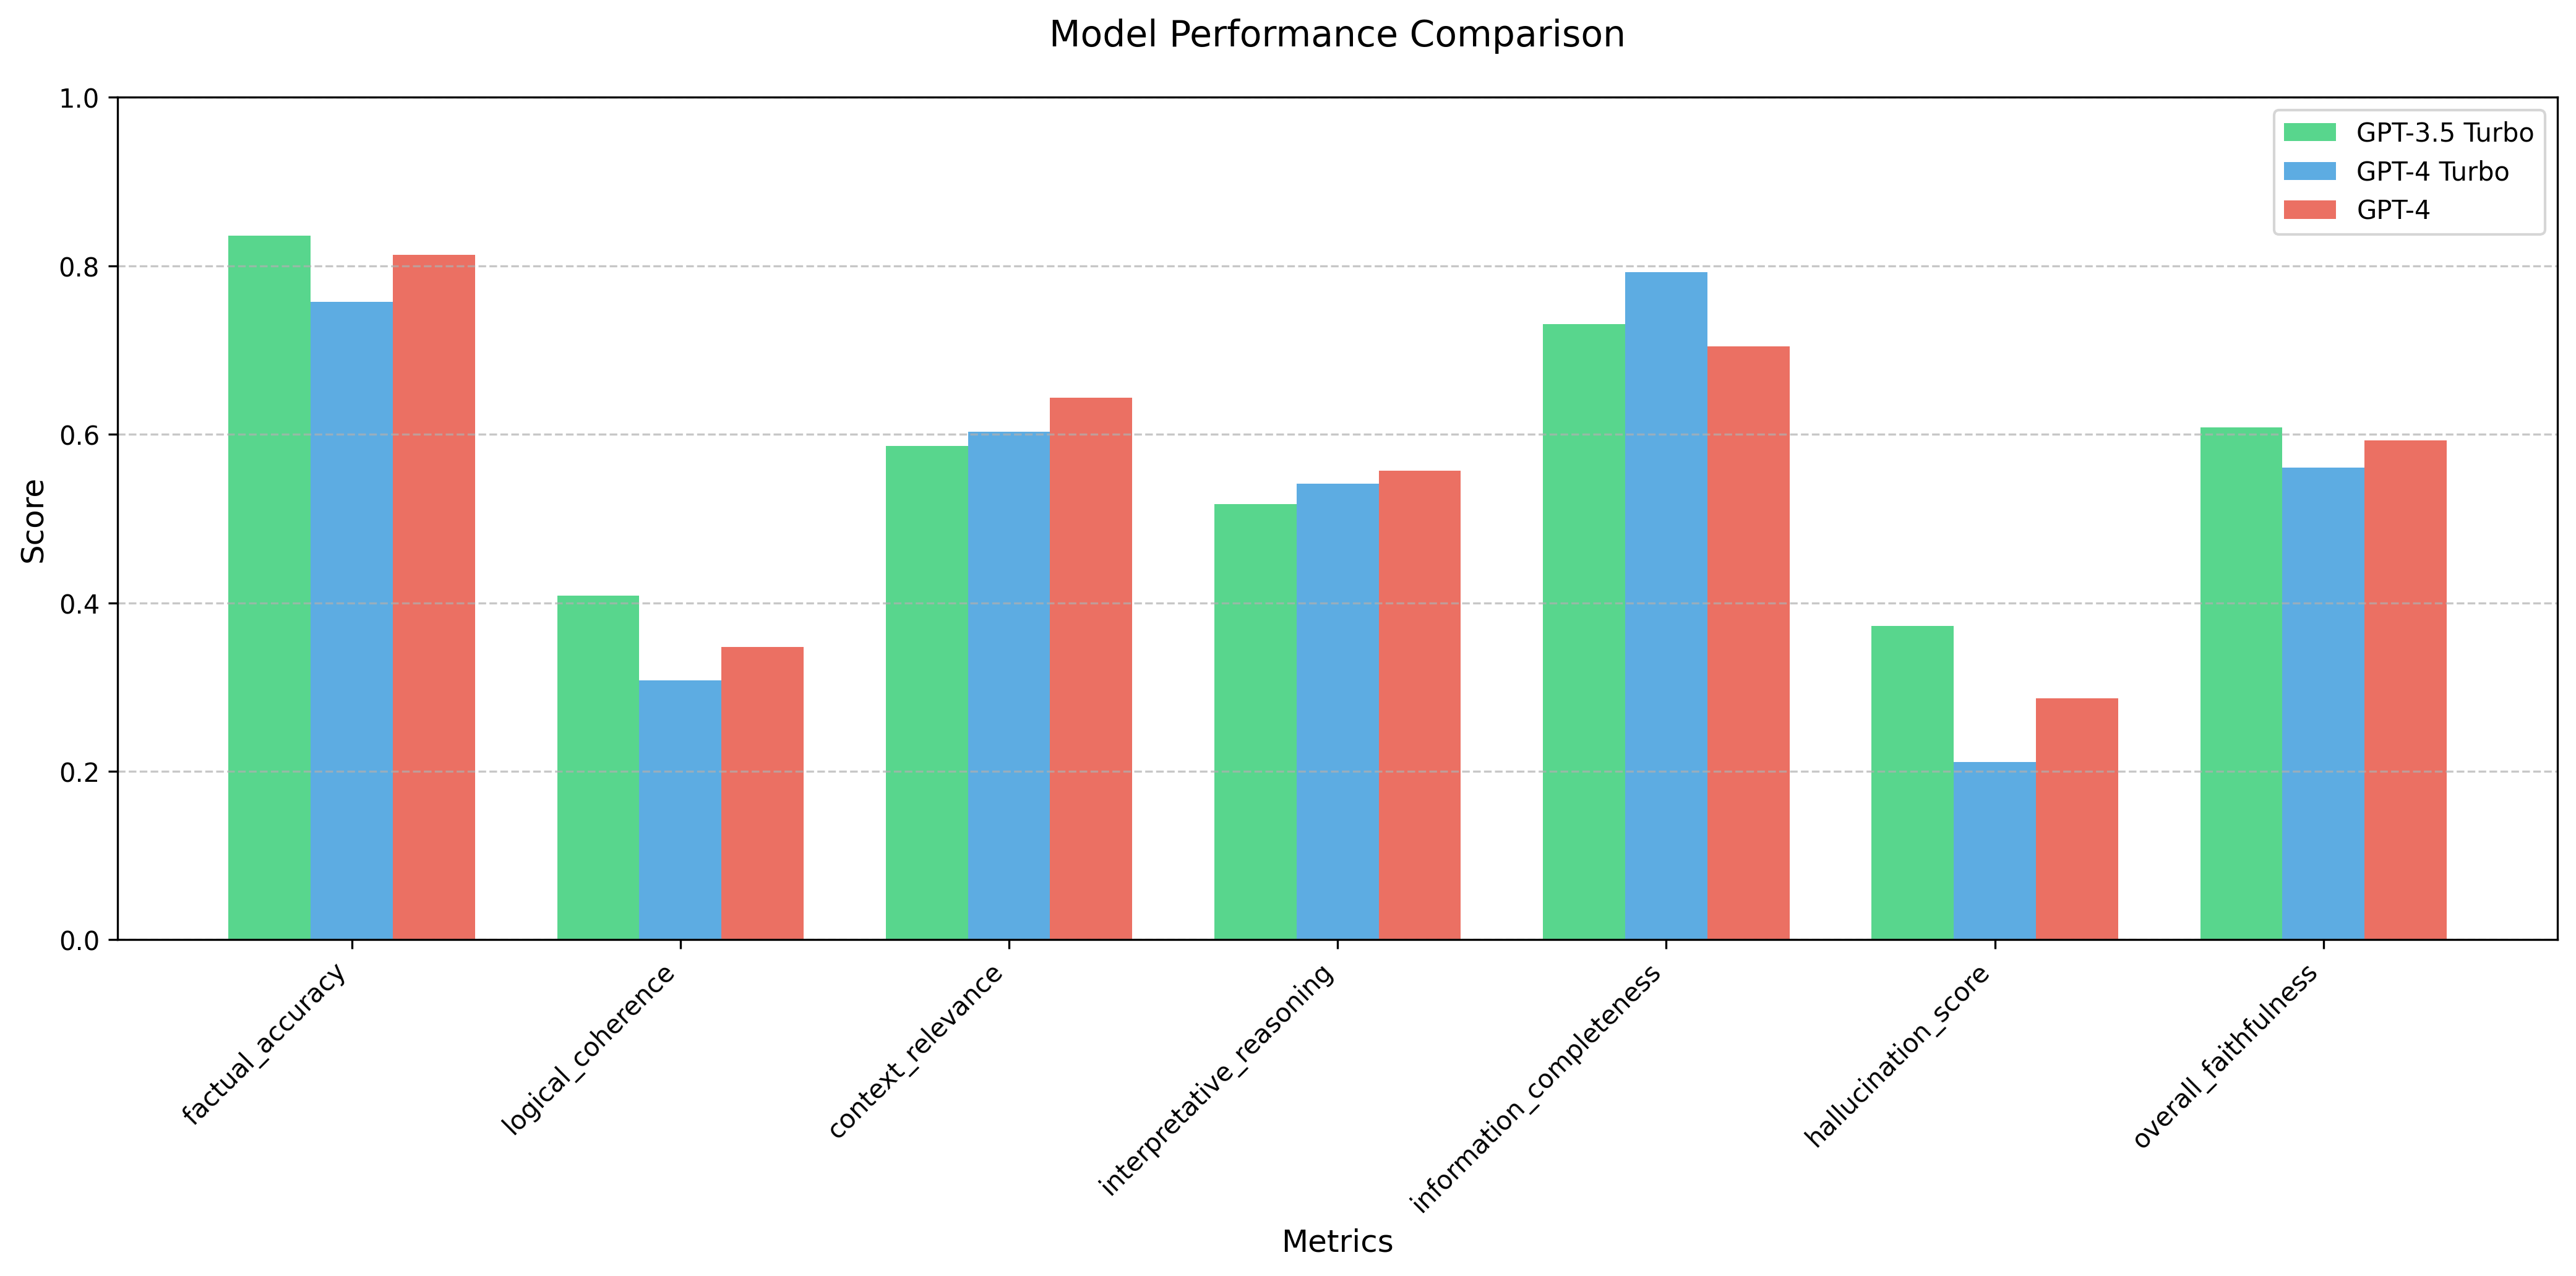
\includegraphics[width=0.8\textwidth]{figures/overall/model_comparison.png}
\caption{Comparative Performance Across Models}
\label{fig:model_comparison}
\end{figure}

The model comparison reveals several interesting patterns:
\begin{itemize}
    \item Factual accuracy remains consistently high across all models (>0.75)
    \item Logical coherence shows the most variation between models
    \item Information completeness demonstrates an inverse relationship with hallucination scores
\end{itemize}

\subsubsection{Overall Metrics Radar Charts}
The radar charts in Figure~\ref{fig:overall_metrics_radar} provide a multidimensional view of each model's performance, highlighting their unique characteristics and balance across different metrics.

\begin{figure}[!htbp]
\centering
\begin{subfigure}{0.3\textwidth}
    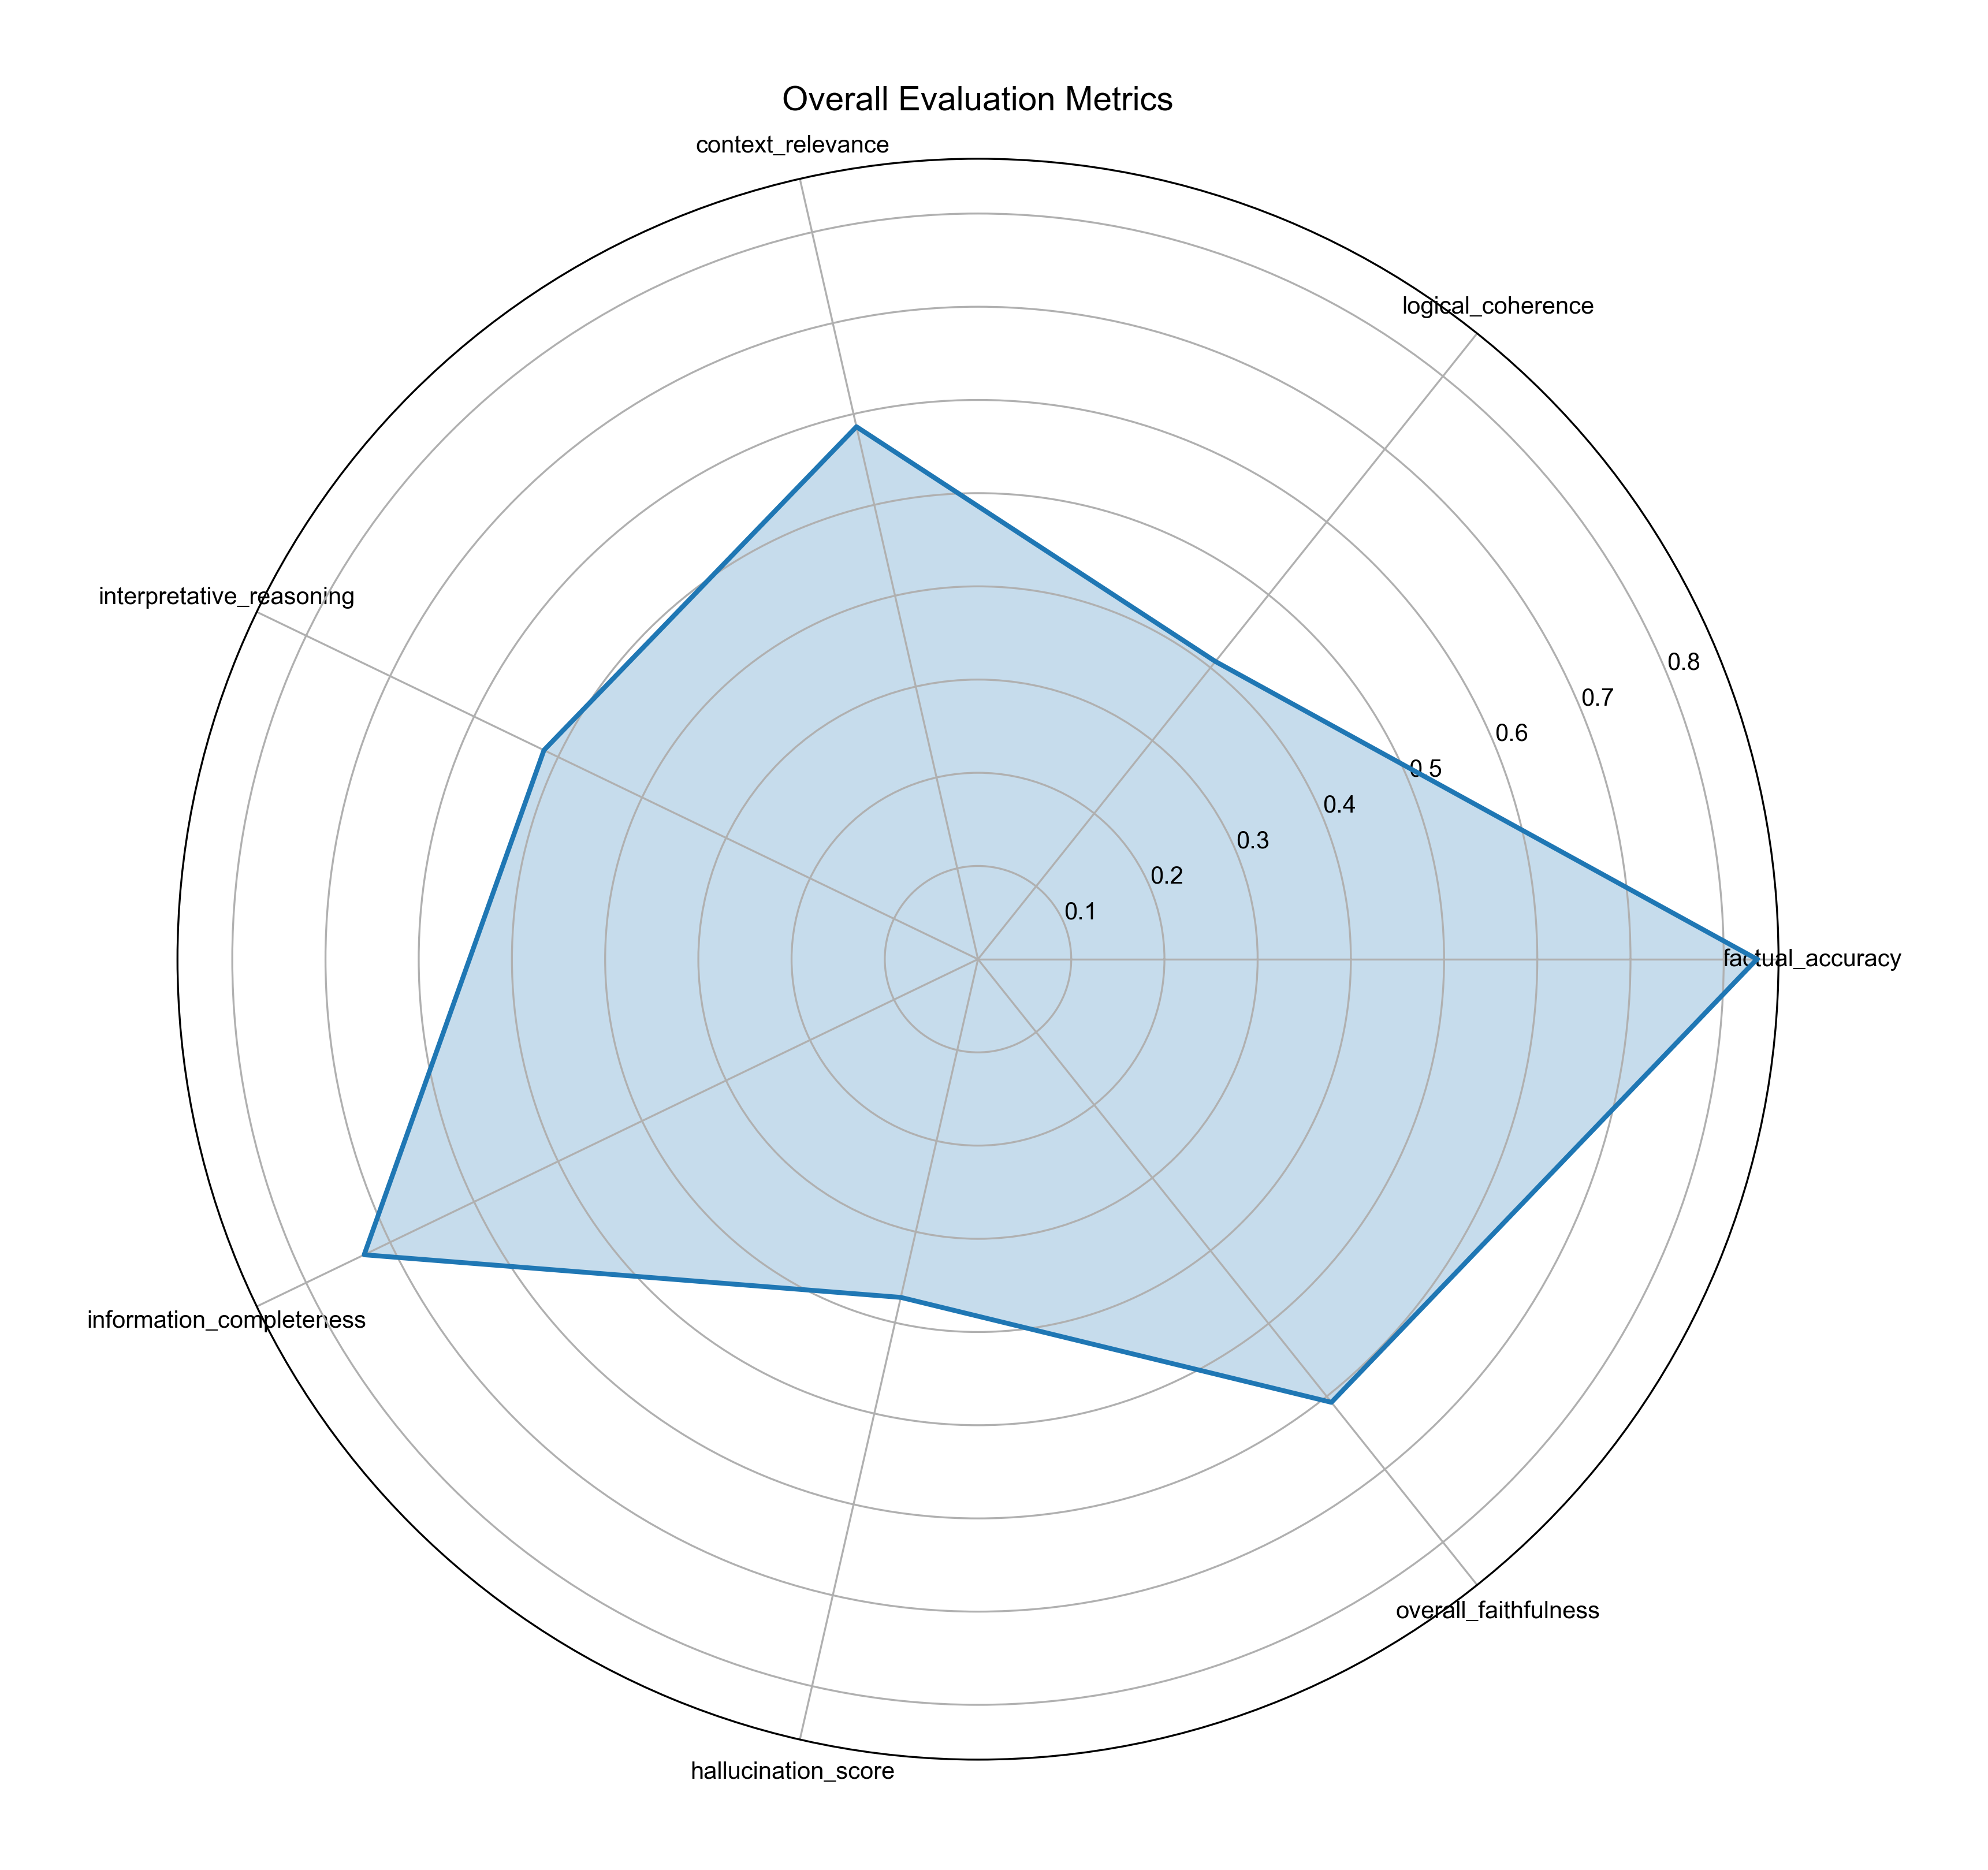
\includegraphics[width=\textwidth]{figures/overall/overall_metrics_radar_gpt-3.5-turbo.png}
    \caption{GPT-3.5-Turbo Metrics}
    \label{fig:overall_metrics_radar_gpt35}
\end{subfigure}
\begin{subfigure}{0.3\textwidth}
    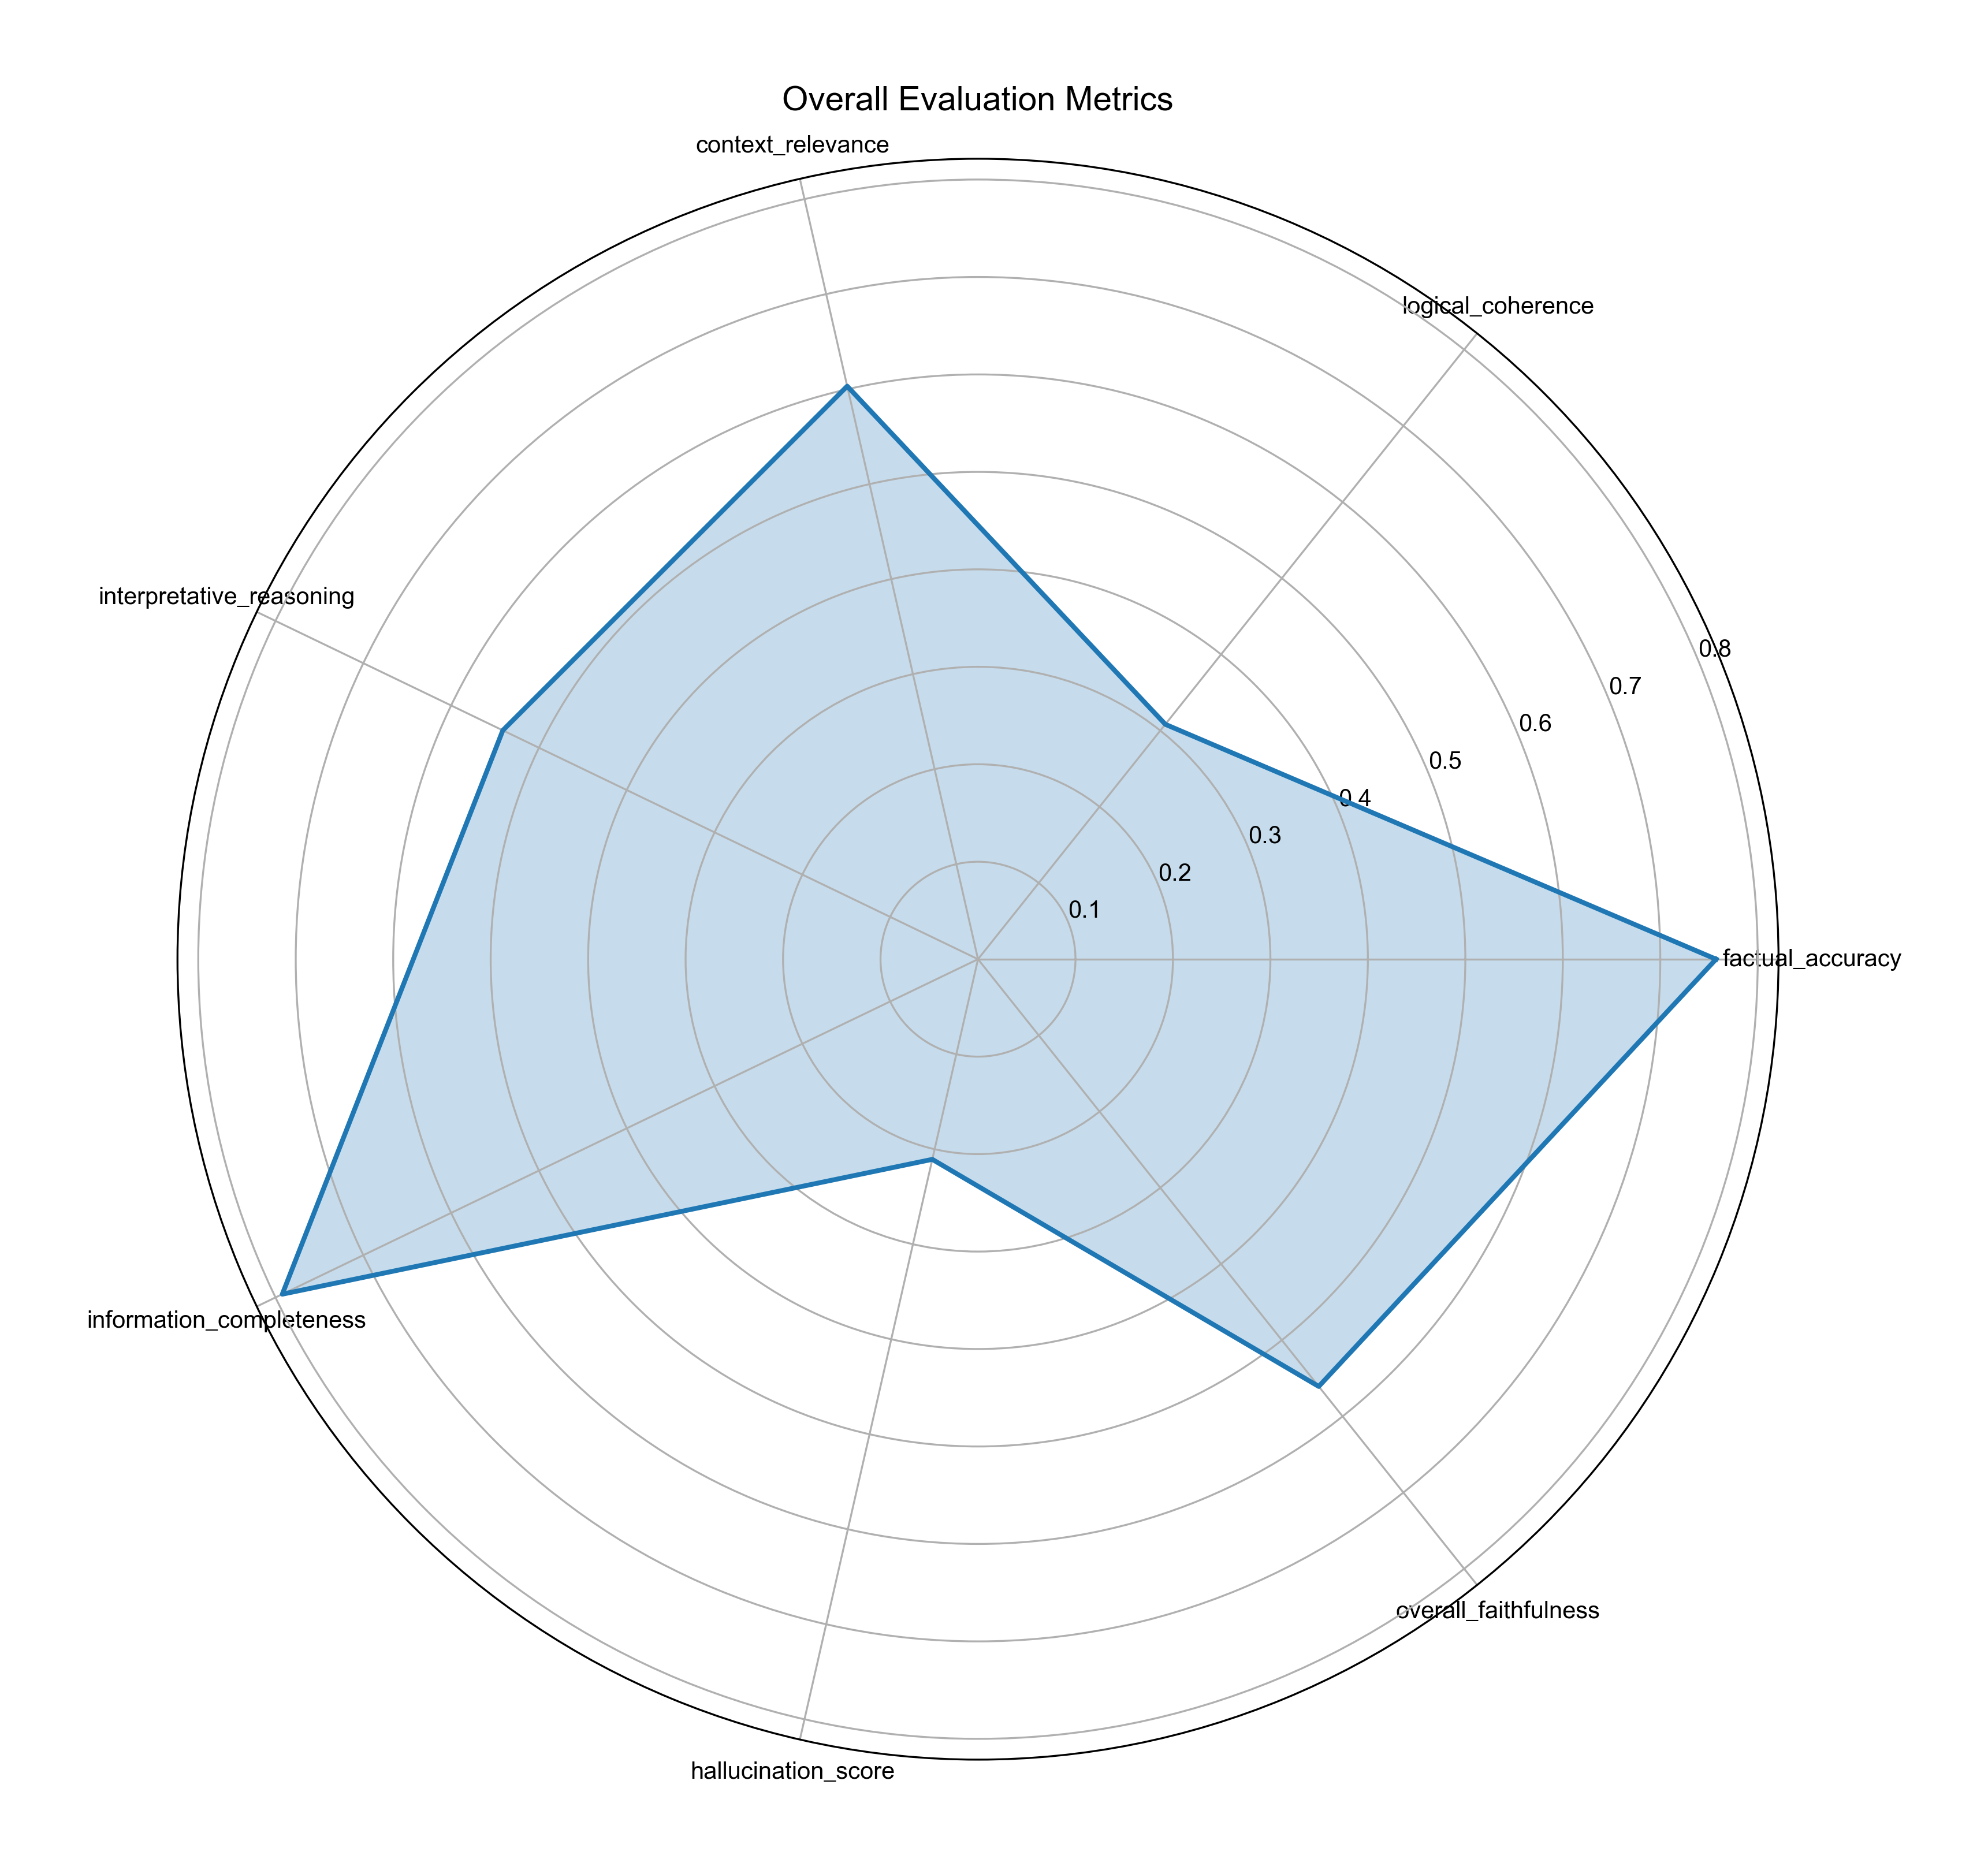
\includegraphics[width=\textwidth]{figures/overall/overall_metrics_radar_gpt-4-turbo.png}
    \caption{GPT-4-Turbo Metrics}
    \label{fig:overall_metrics_radar_gpt4t}
\end{subfigure}
\begin{subfigure}{0.3\textwidth}
    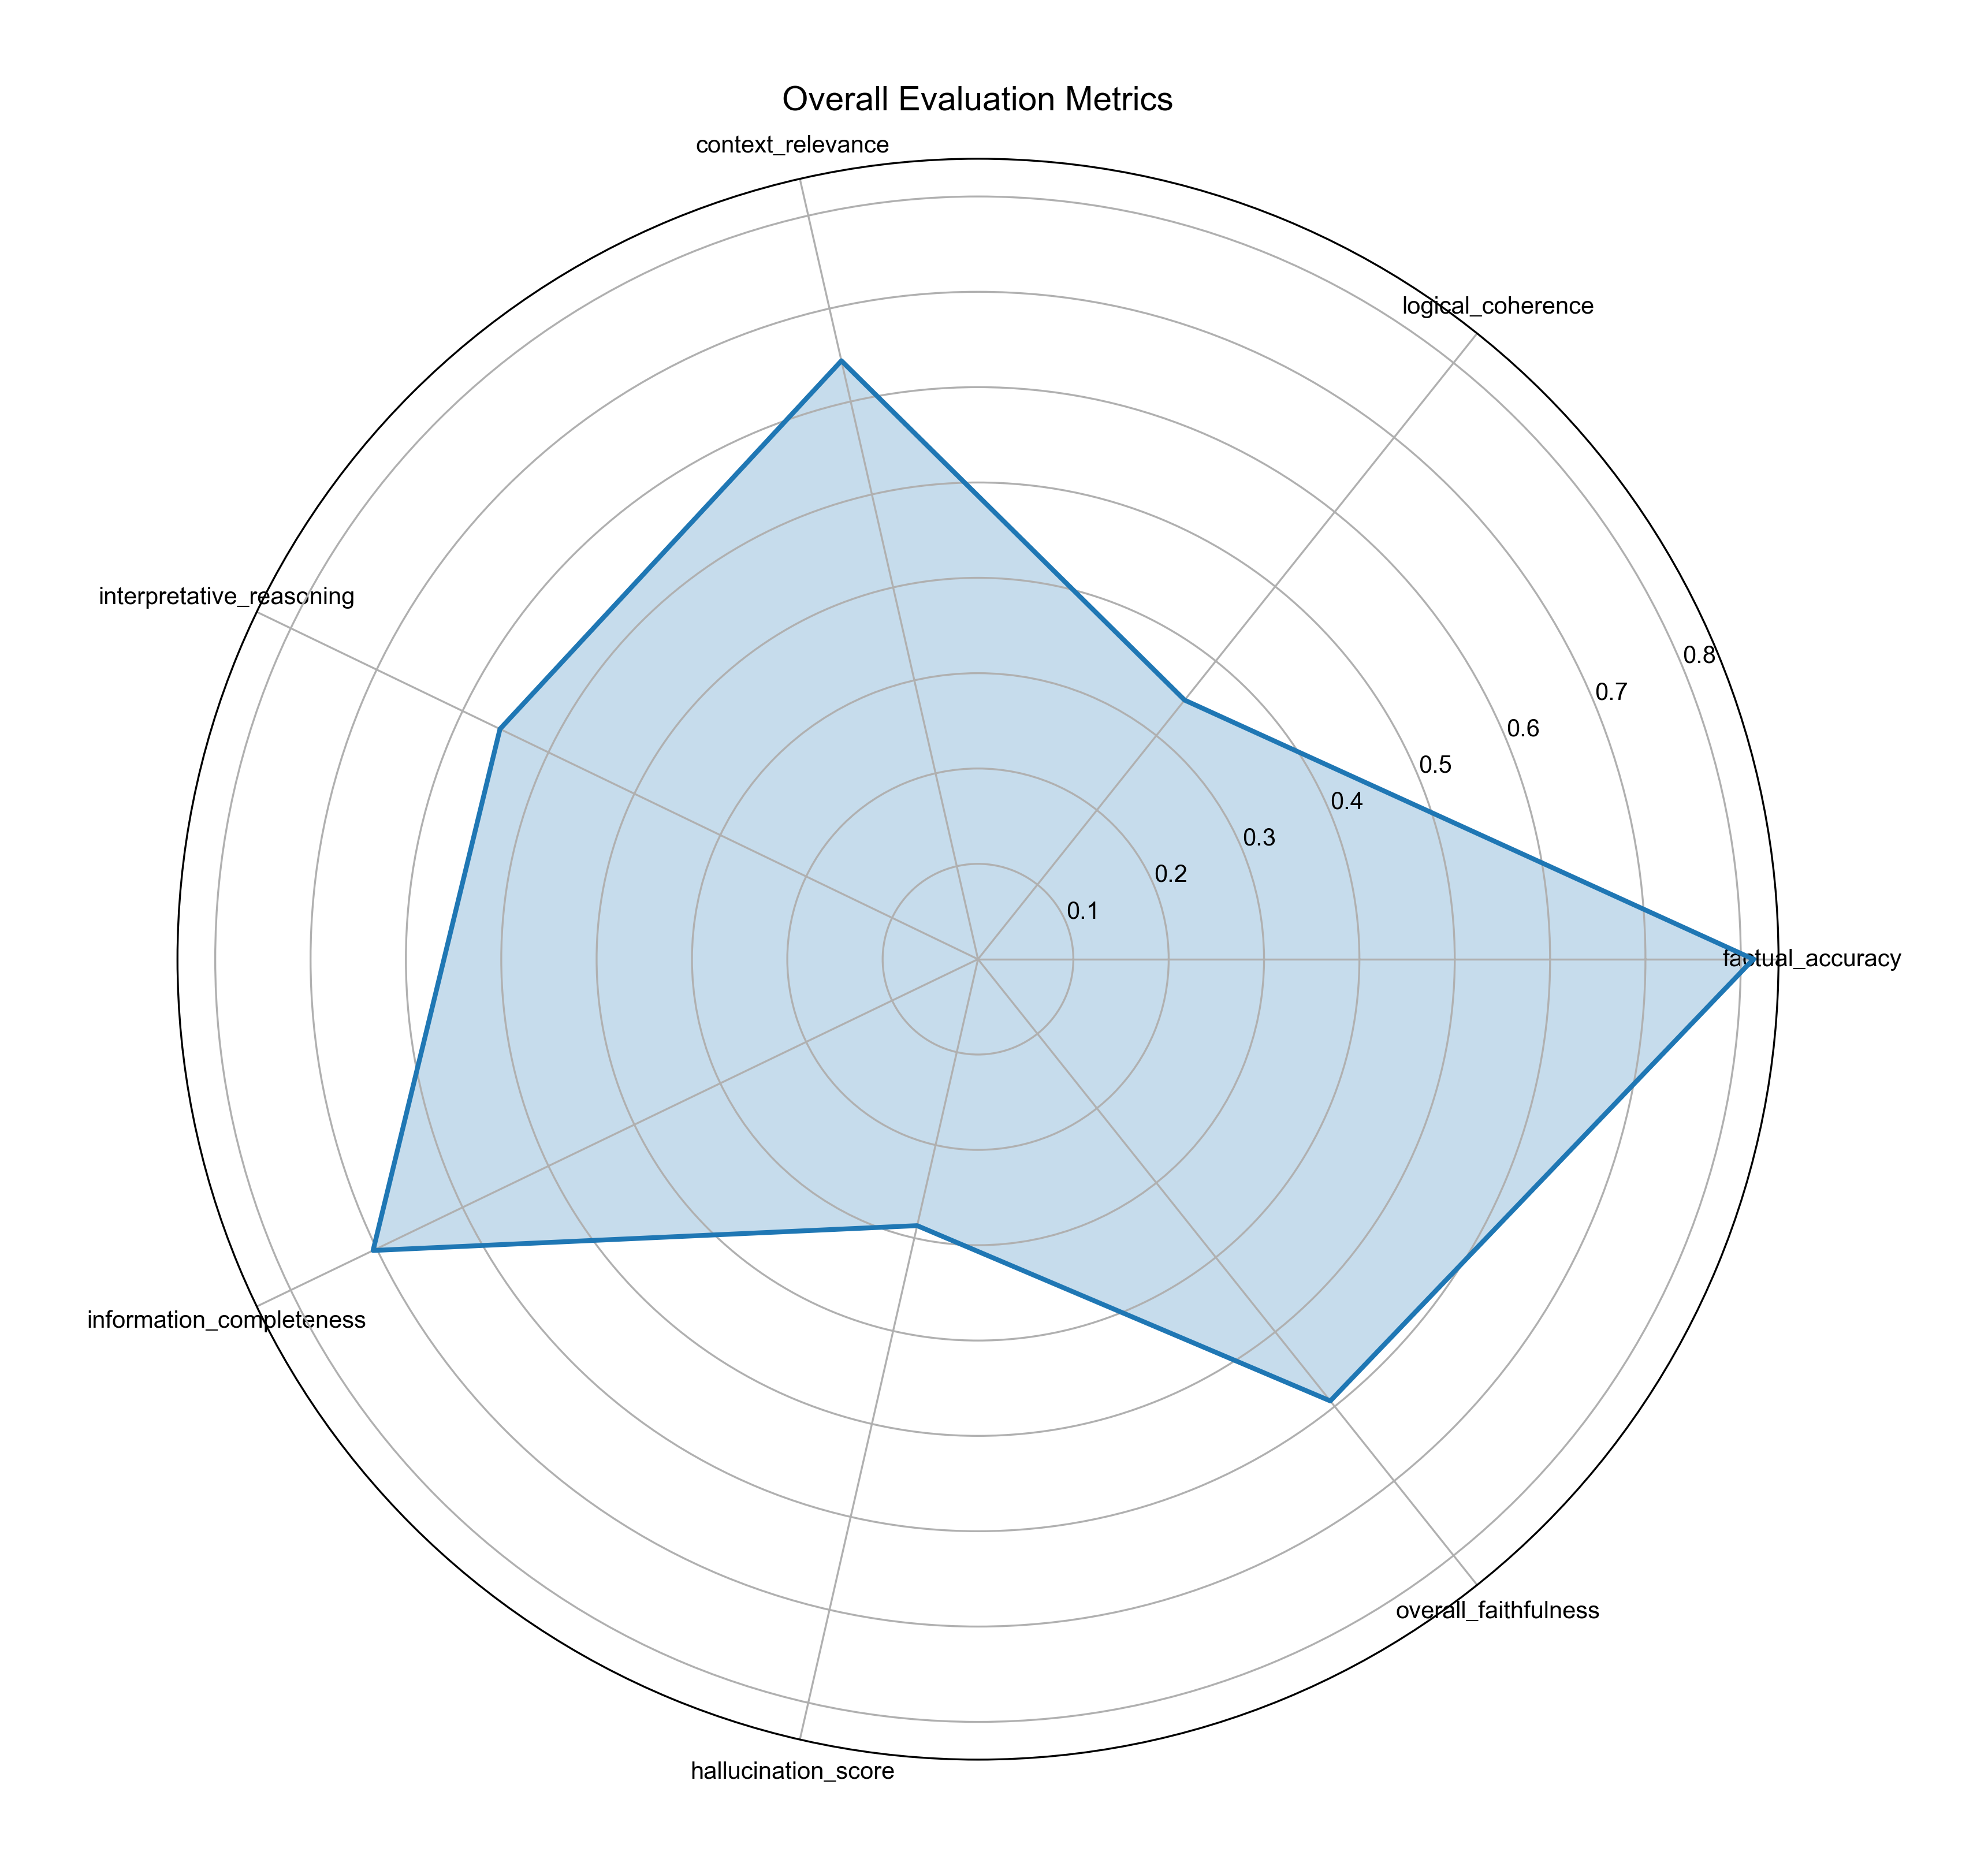
\includegraphics[width=\textwidth]{figures/overall/overall_metrics_radar_gpt-4.png}
    \caption{GPT-4 Metrics}
    \label{fig:overall_metrics_radar_gpt4}
\end{subfigure}
\caption{Overall Metrics Radar Charts by Model}
\label{fig:overall_metrics_radar}
\end{figure}

\textbf{Radar Chart Analysis}:
\begin{itemize}
    \item Each model exhibits distinct patterns in their metric distribution
    \item GPT-3.5-Turbo shows more balanced performance across metrics
    \item GPT-4 variants demonstrate stronger performance in specific areas
\end{itemize}

\subsubsection{Metrics Trend Analysis}
Building on our methodology described in Section~\ref{sec:methodology}, we analyzed the evolution of different metrics across various evaluation scenarios for each model, providing insights into their performance stability and patterns.

\begin{figure}[!htbp]
\centering
\begin{subfigure}{0.3\textwidth}
    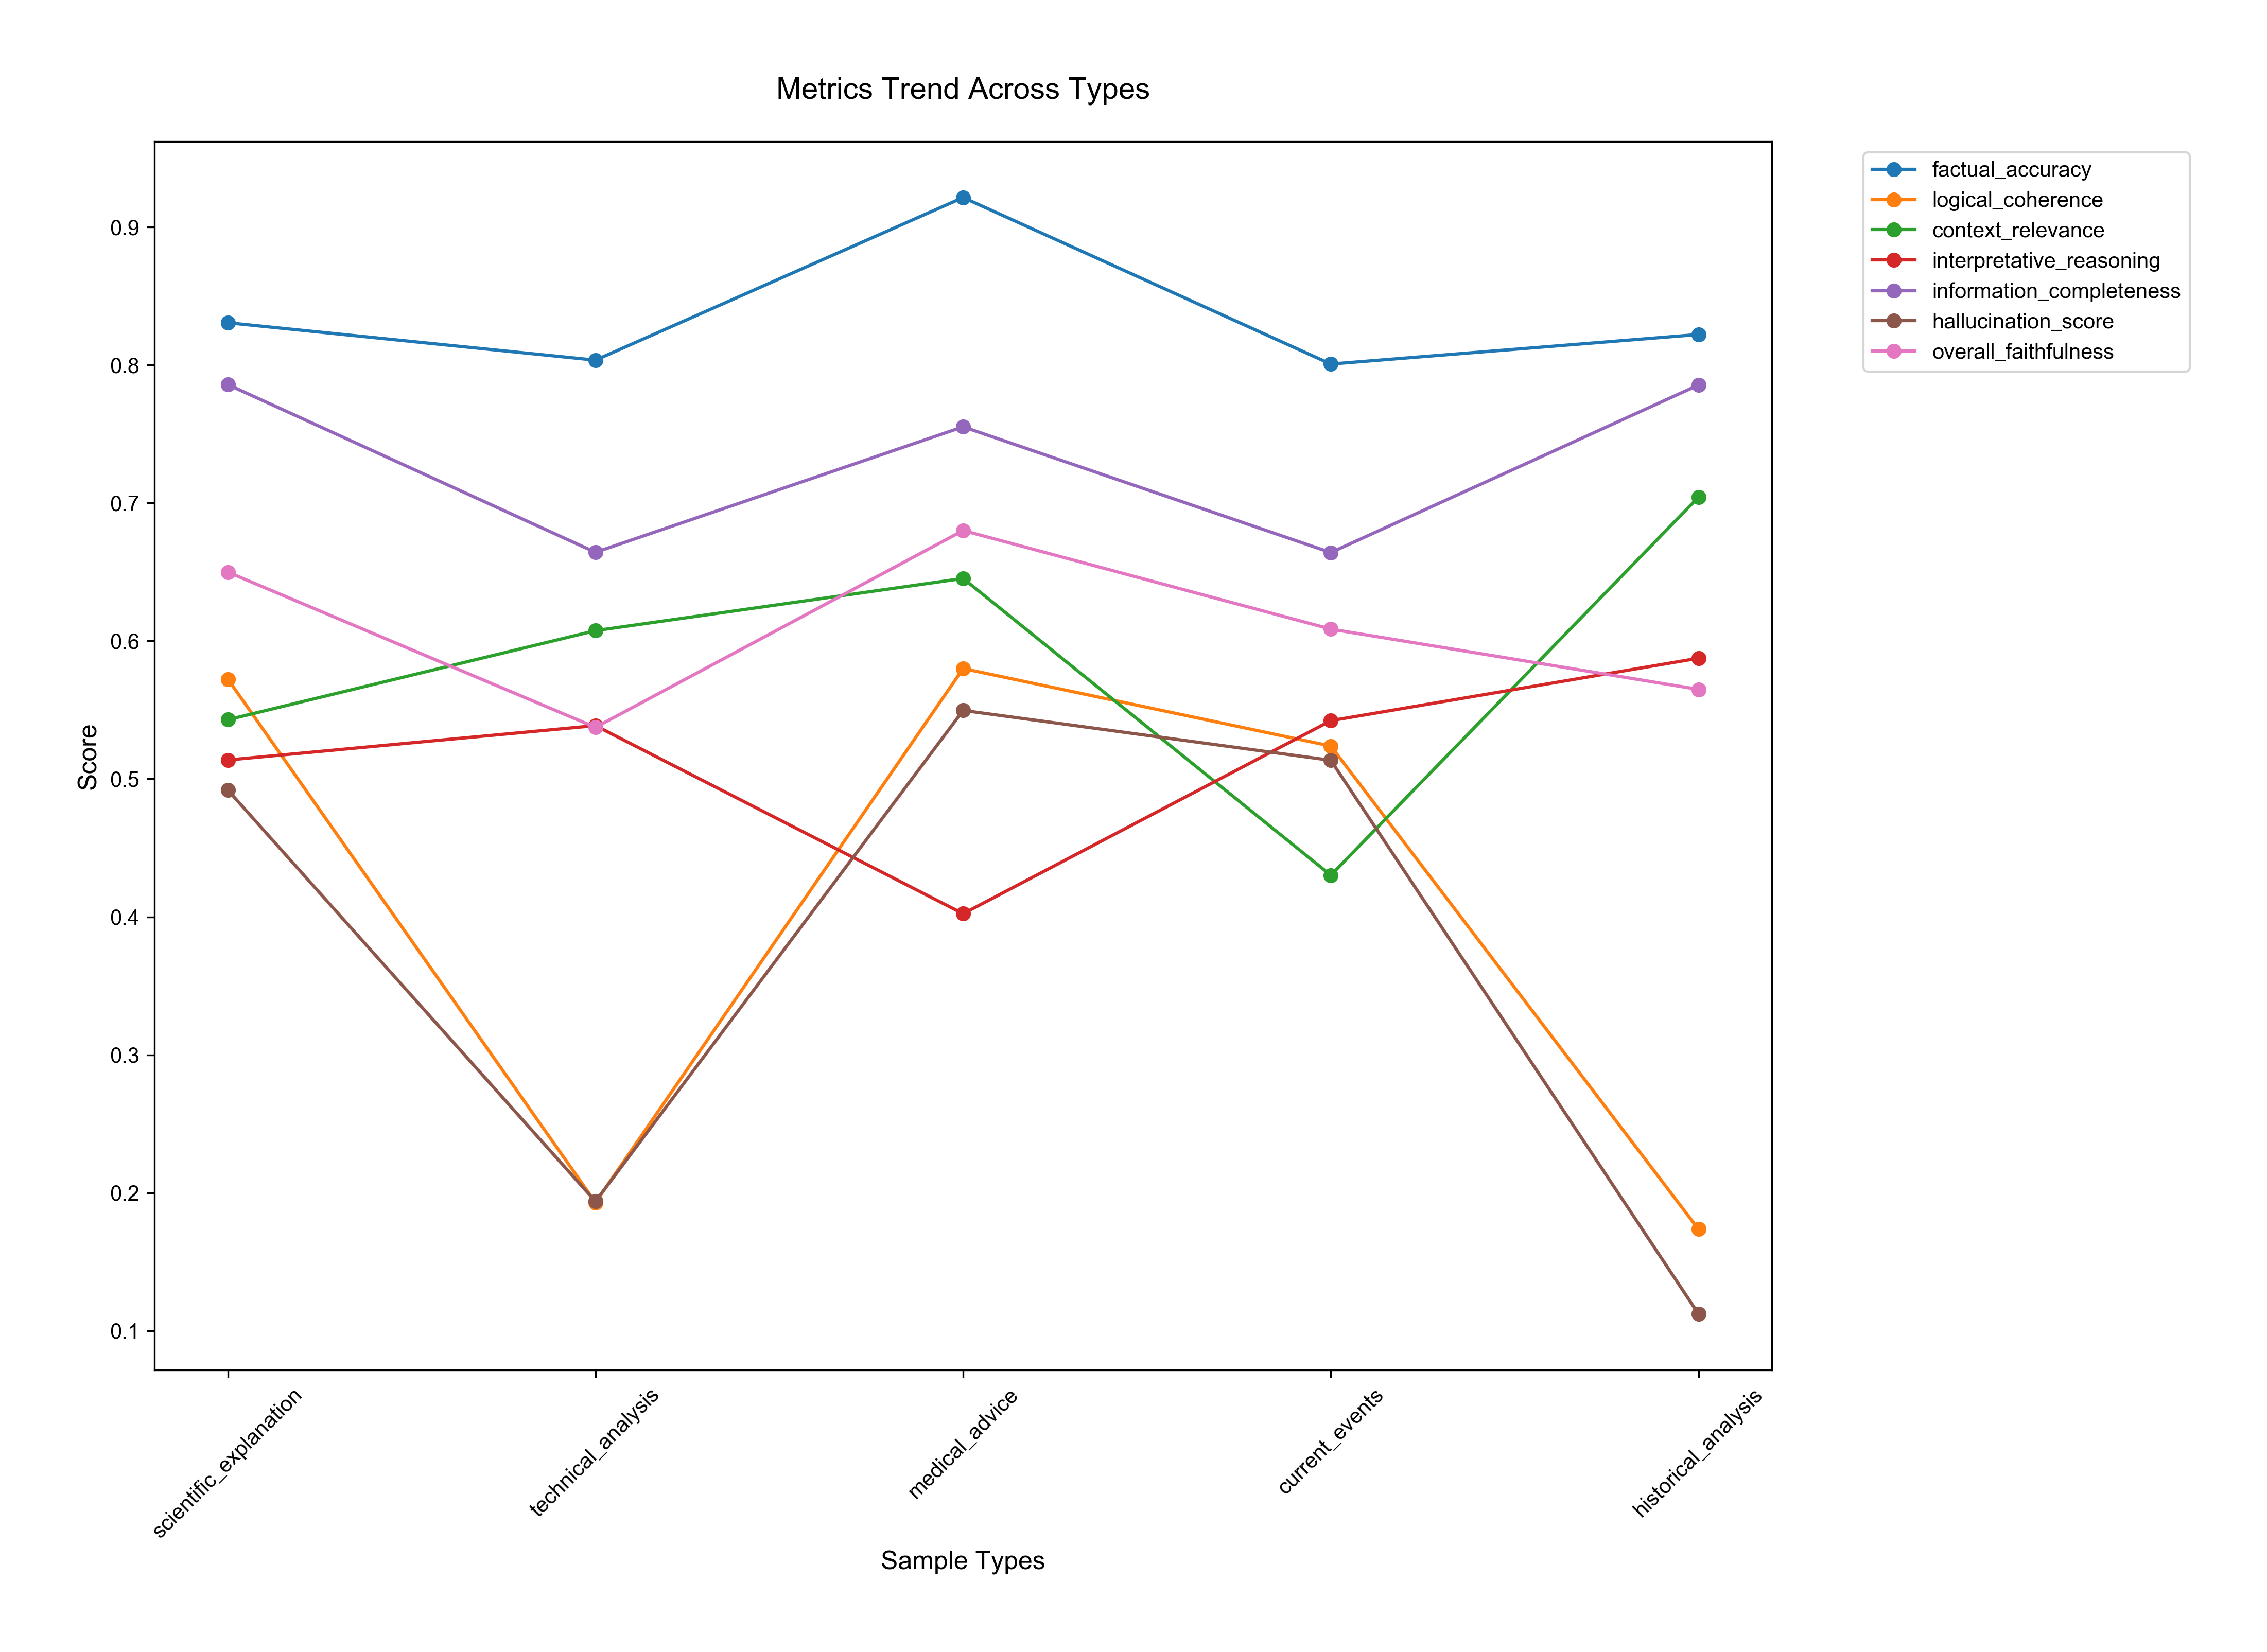
\includegraphics[width=\textwidth]{figures/overall/metrics_trend_gpt-3.5-turbo.png}
    \caption{GPT-3.5-Turbo Trends}
    \label{fig:metrics_trend_gpt35}
\end{subfigure}
\begin{subfigure}{0.3\textwidth}
    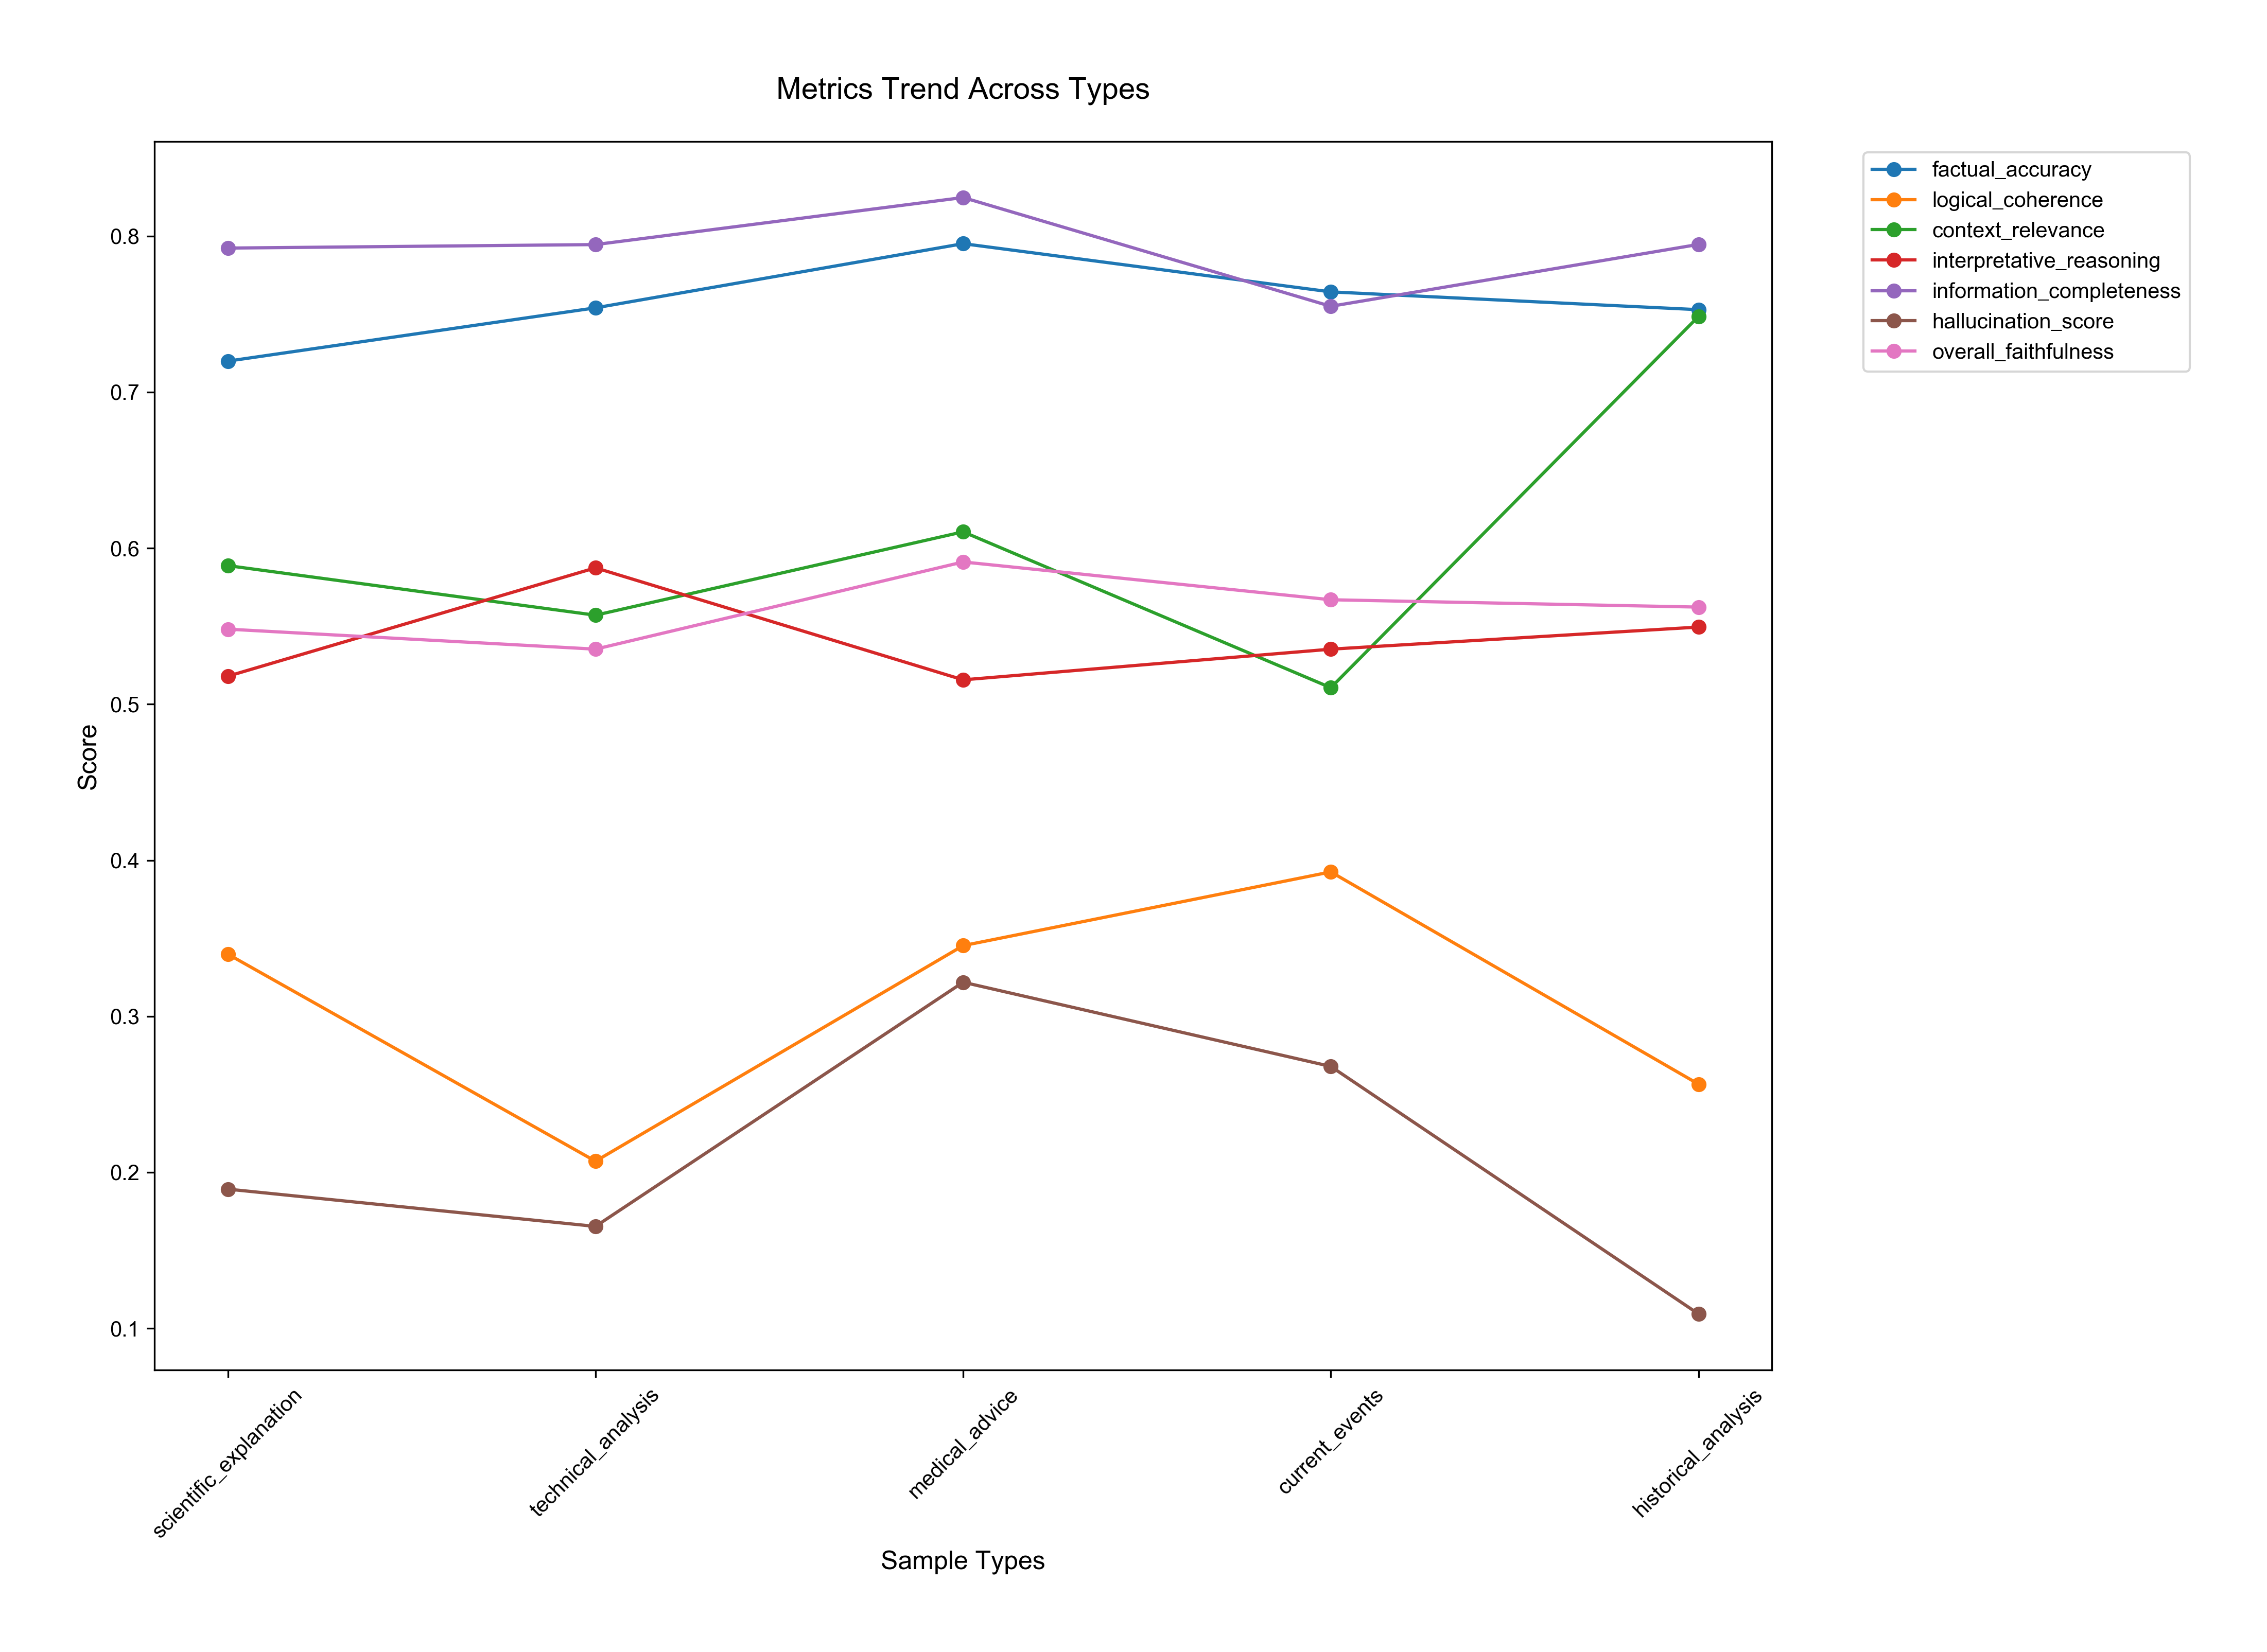
\includegraphics[width=\textwidth]{figures/overall/metrics_trend_gpt-4-turbo.png}
    \caption{GPT-4-Turbo Trends}
    \label{fig:metrics_trend_gpt4t}
\end{subfigure}
\begin{subfigure}{0.3\textwidth}
    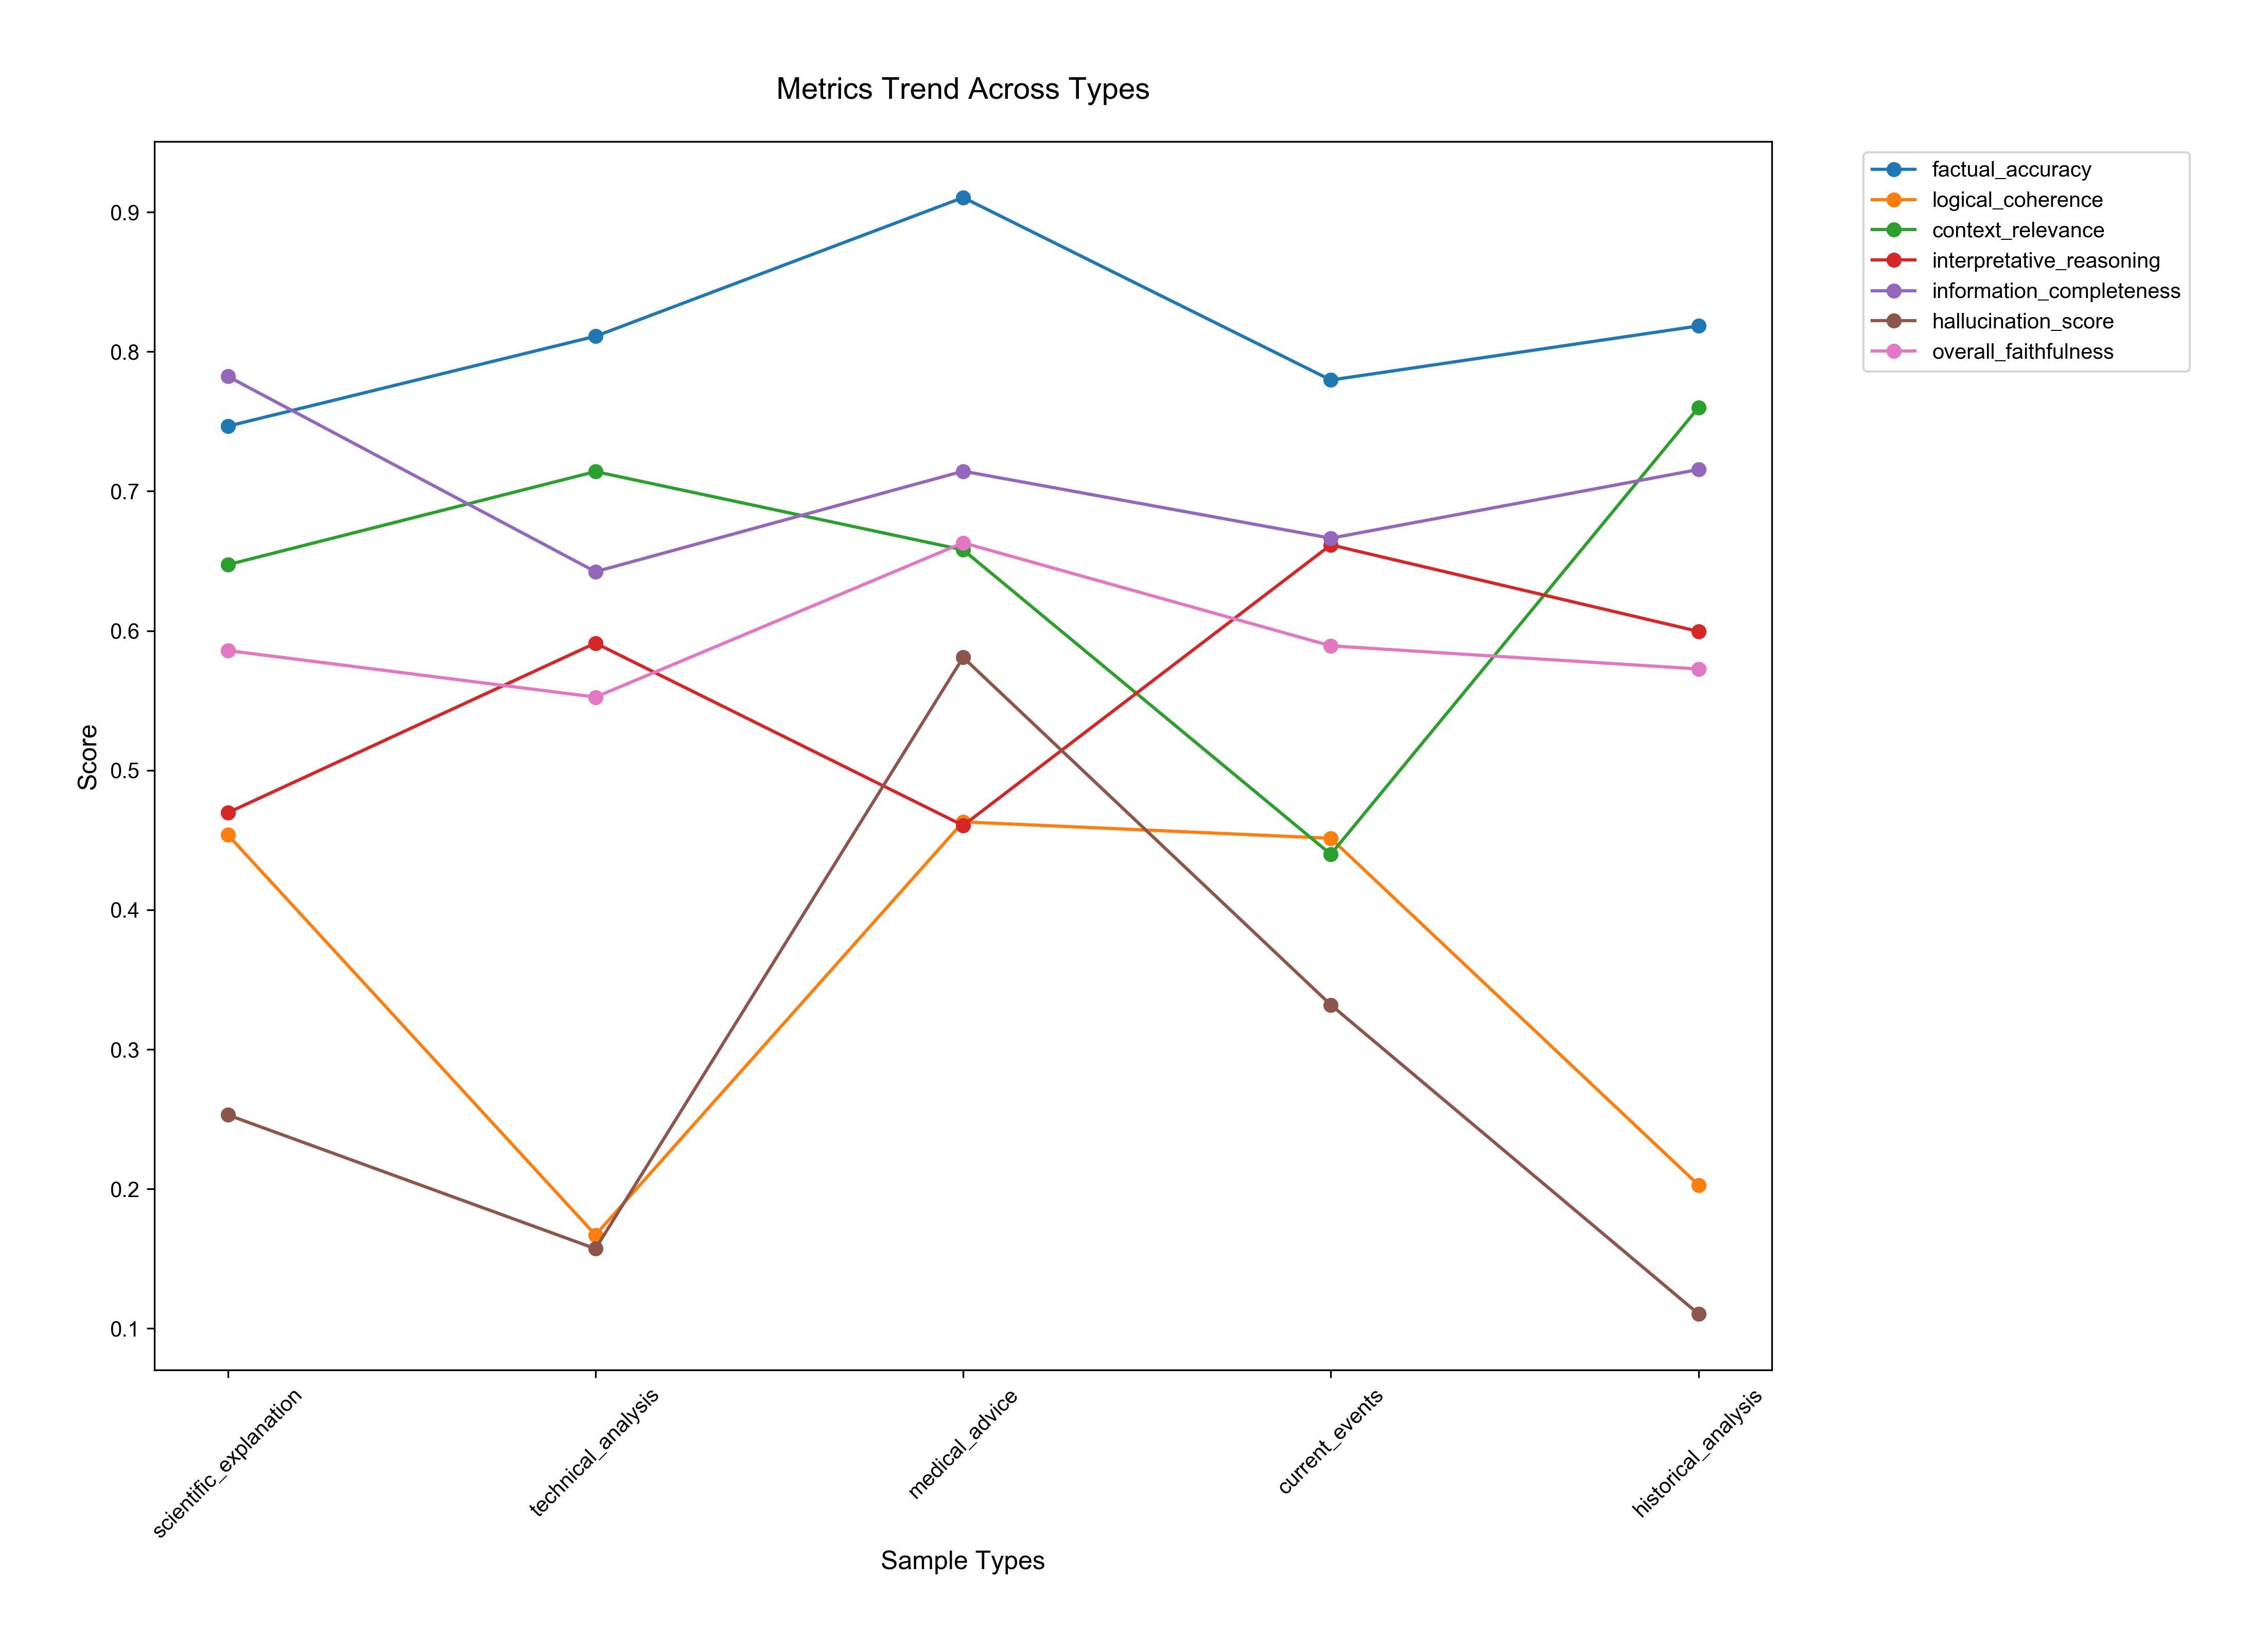
\includegraphics[width=\textwidth]{figures/overall/metrics_trend_gpt-4.png}
    \caption{GPT-4 Trends}
    \label{fig:metrics_trend_gpt4}
\end{subfigure}
\caption{Metrics Trend Analysis by Model}
\label{fig:metrics_trends}
\end{figure}

\textbf{Key Trend Observations}:
\begin{itemize}
    \item \textbf{Factual Accuracy}: Shows consistent high performance across all models, with minor fluctuations
    \item \textbf{Logical Coherence}: Exhibits the most variability, particularly in complex scenarios
    \item \textbf{Context Relevance}: Demonstrates steady improvement as models process more context
    \item \textbf{Hallucination Scores}: Show decreasing trends, indicating better control over fabricated information
\end{itemize}

\subsection{Type-Specific Evaluation Results}
Our analysis extends to different content types, revealing how models perform across various domains and contexts.

\subsubsection{Scientific Explanation}
The evaluation of scientific explanations focuses on the models' ability to accurately convey complex scientific concepts while maintaining factual integrity.

\begin{table}[!htbp]
\centering
\setlength{\tabcolsep}{4pt}  % Reduce table column spacing
\begin{tabular}{|l|c|c|c|c|c|c|c|}
\hline
\textbf{Model} & \textbf{FA} & \textbf{LC} & \textbf{CR} & \textbf{IR} 
& \textbf{IC} & \textbf{HS} & \textbf{OF} \\
\hline
GPT-3.5-Turbo & 0.83 & 0.57 & 0.54 & 0.51 & 0.79 & 0.49 & 0.65 \\
GPT-4-Turbo & 0.72 & 0.34 & 0.59 & 0.52 & 0.79 & 0.19 & 0.55 \\
GPT-4 & 0.75 & 0.45 & 0.65 & 0.47 & 0.78 & 0.25 & 0.59 \\
\hline
\end{tabular}
\caption{Scientific Explanation Metrics}
\label{tab:results_scientific_metrics}
\begin{flushleft}
\small
FA: Factual Accuracy, LC: Logical Coherence, CR: Context Relevance,\\
IR: Interpretative Reasoning, IC: Information Completeness, HS: Hallucination Score, OF: Overall Faithfulness
\end{flushleft}
\end{table}

\begin{figure}[!htbp]
\centering
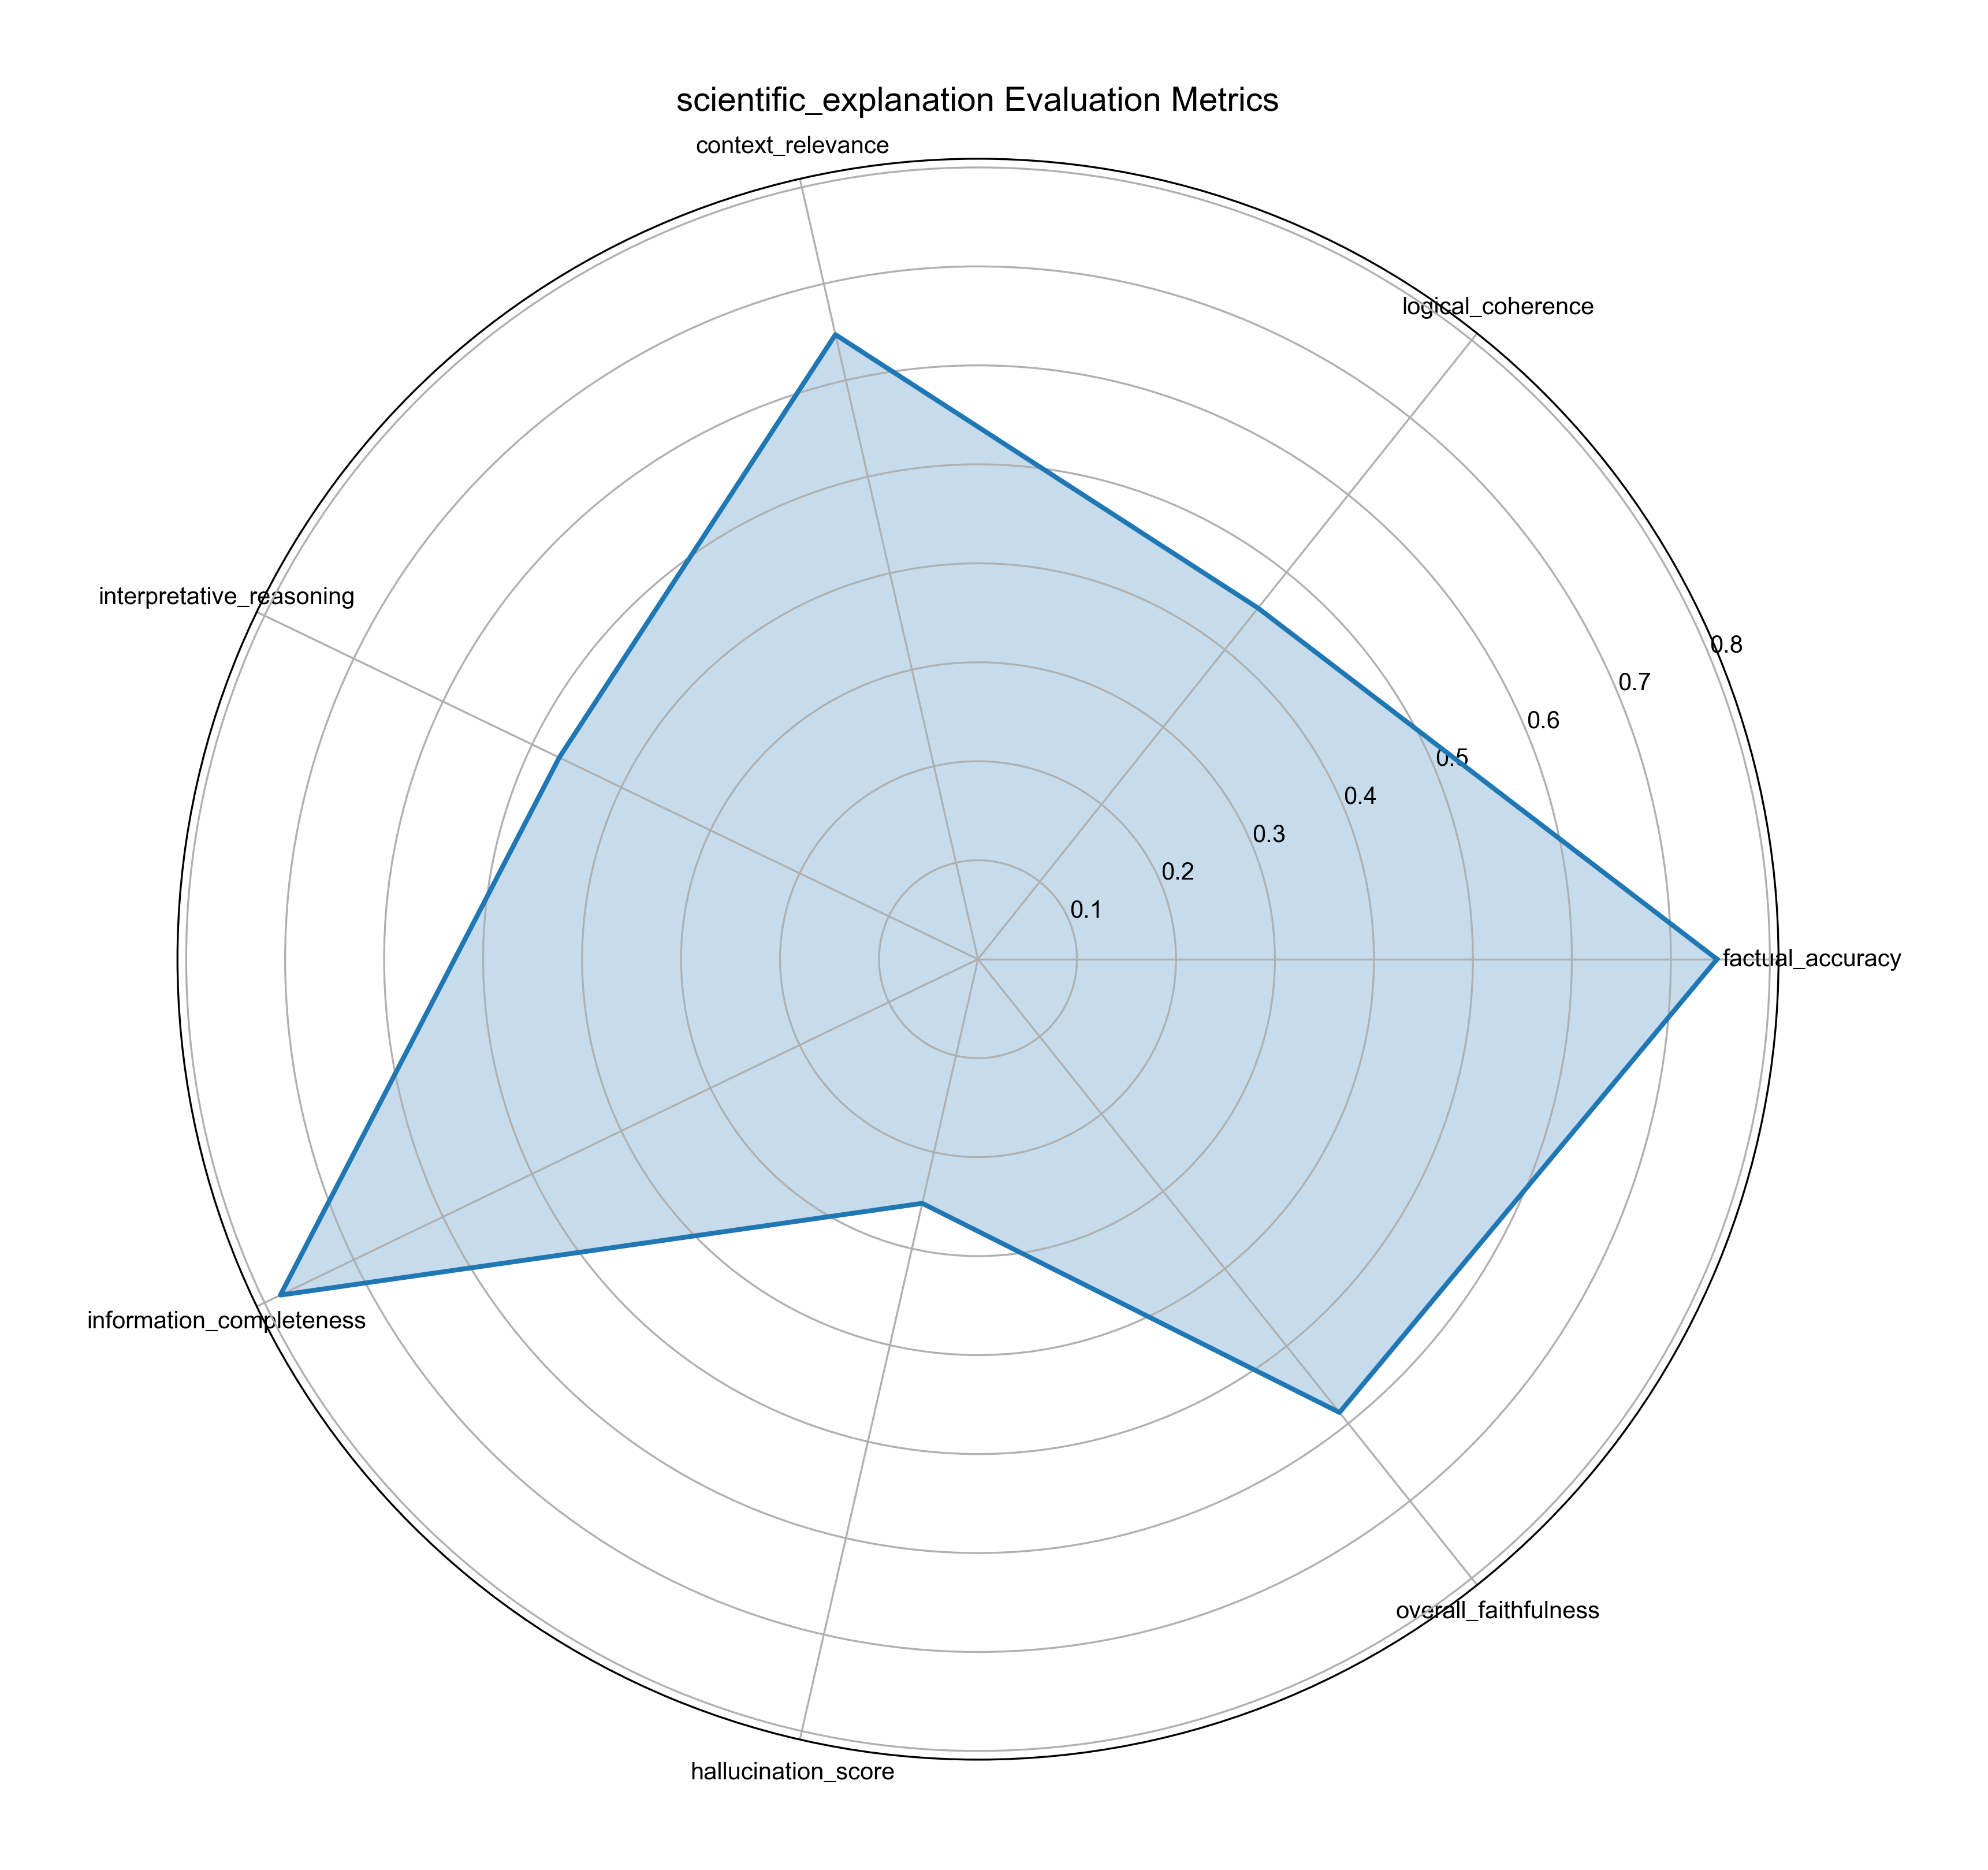
\includegraphics[width=0.6\textwidth]{figures/types/scientific_explanation_radar_gpt-4.png}
\caption{Scientific Explanation Performance Radar}
\label{fig:scientific_radar}
\end{figure}

\textbf{Analysis}:
\begin{itemize}
    \item GPT-3.5-Turbo demonstrates exceptional performance in scientific explanations, particularly in factual accuracy (0.83) and information completeness (0.79)
    \item Higher hallucination scores in this category suggest challenges in maintaining strict factual boundaries
    \item Logical coherence scores indicate room for improvement in structuring scientific arguments
\end{itemize}

\subsubsection{Technical Analysis}
For technical content, we evaluated the models' capability to handle detailed technical information and maintain accuracy in specialized contexts.

\begin{table}[!htbp]
\centering
\setlength{\tabcolsep}{4pt}  % Reduce table column spacing
\begin{tabular}{|l|c|c|c|c|c|c|c|}
\hline
\textbf{Model} & \textbf{FA} & \textbf{LC} & \textbf{CR} & \textbf{IR} 
& \textbf{IC} & \textbf{HS} & \textbf{OF} \\
\hline
GPT-3.5-Turbo & 0.80 & 0.19 & 0.61 & 0.54 & 0.66 & 0.19 & 0.54 \\
GPT-4-Turbo & 0.75 & 0.21 & 0.56 & 0.59 & 0.79 & 0.17 & 0.54 \\
GPT-4 & 0.81 & 0.17 & 0.71 & 0.59 & 0.64 & 0.16 & 0.55 \\
\hline
\end{tabular}
\caption{Technical Analysis Metrics}
\label{tab:results_technical_metrics}
\begin{flushleft}
\small
FA: Factual Accuracy, LC: Logical Coherence, CR: Context Relevance,\\
IR: Interpretative Reasoning, IC: Information Completeness, HS: Hallucination Score, OF: Overall Faithfulness
\end{flushleft}
\end{table}

\begin{figure}[!htbp]
\centering
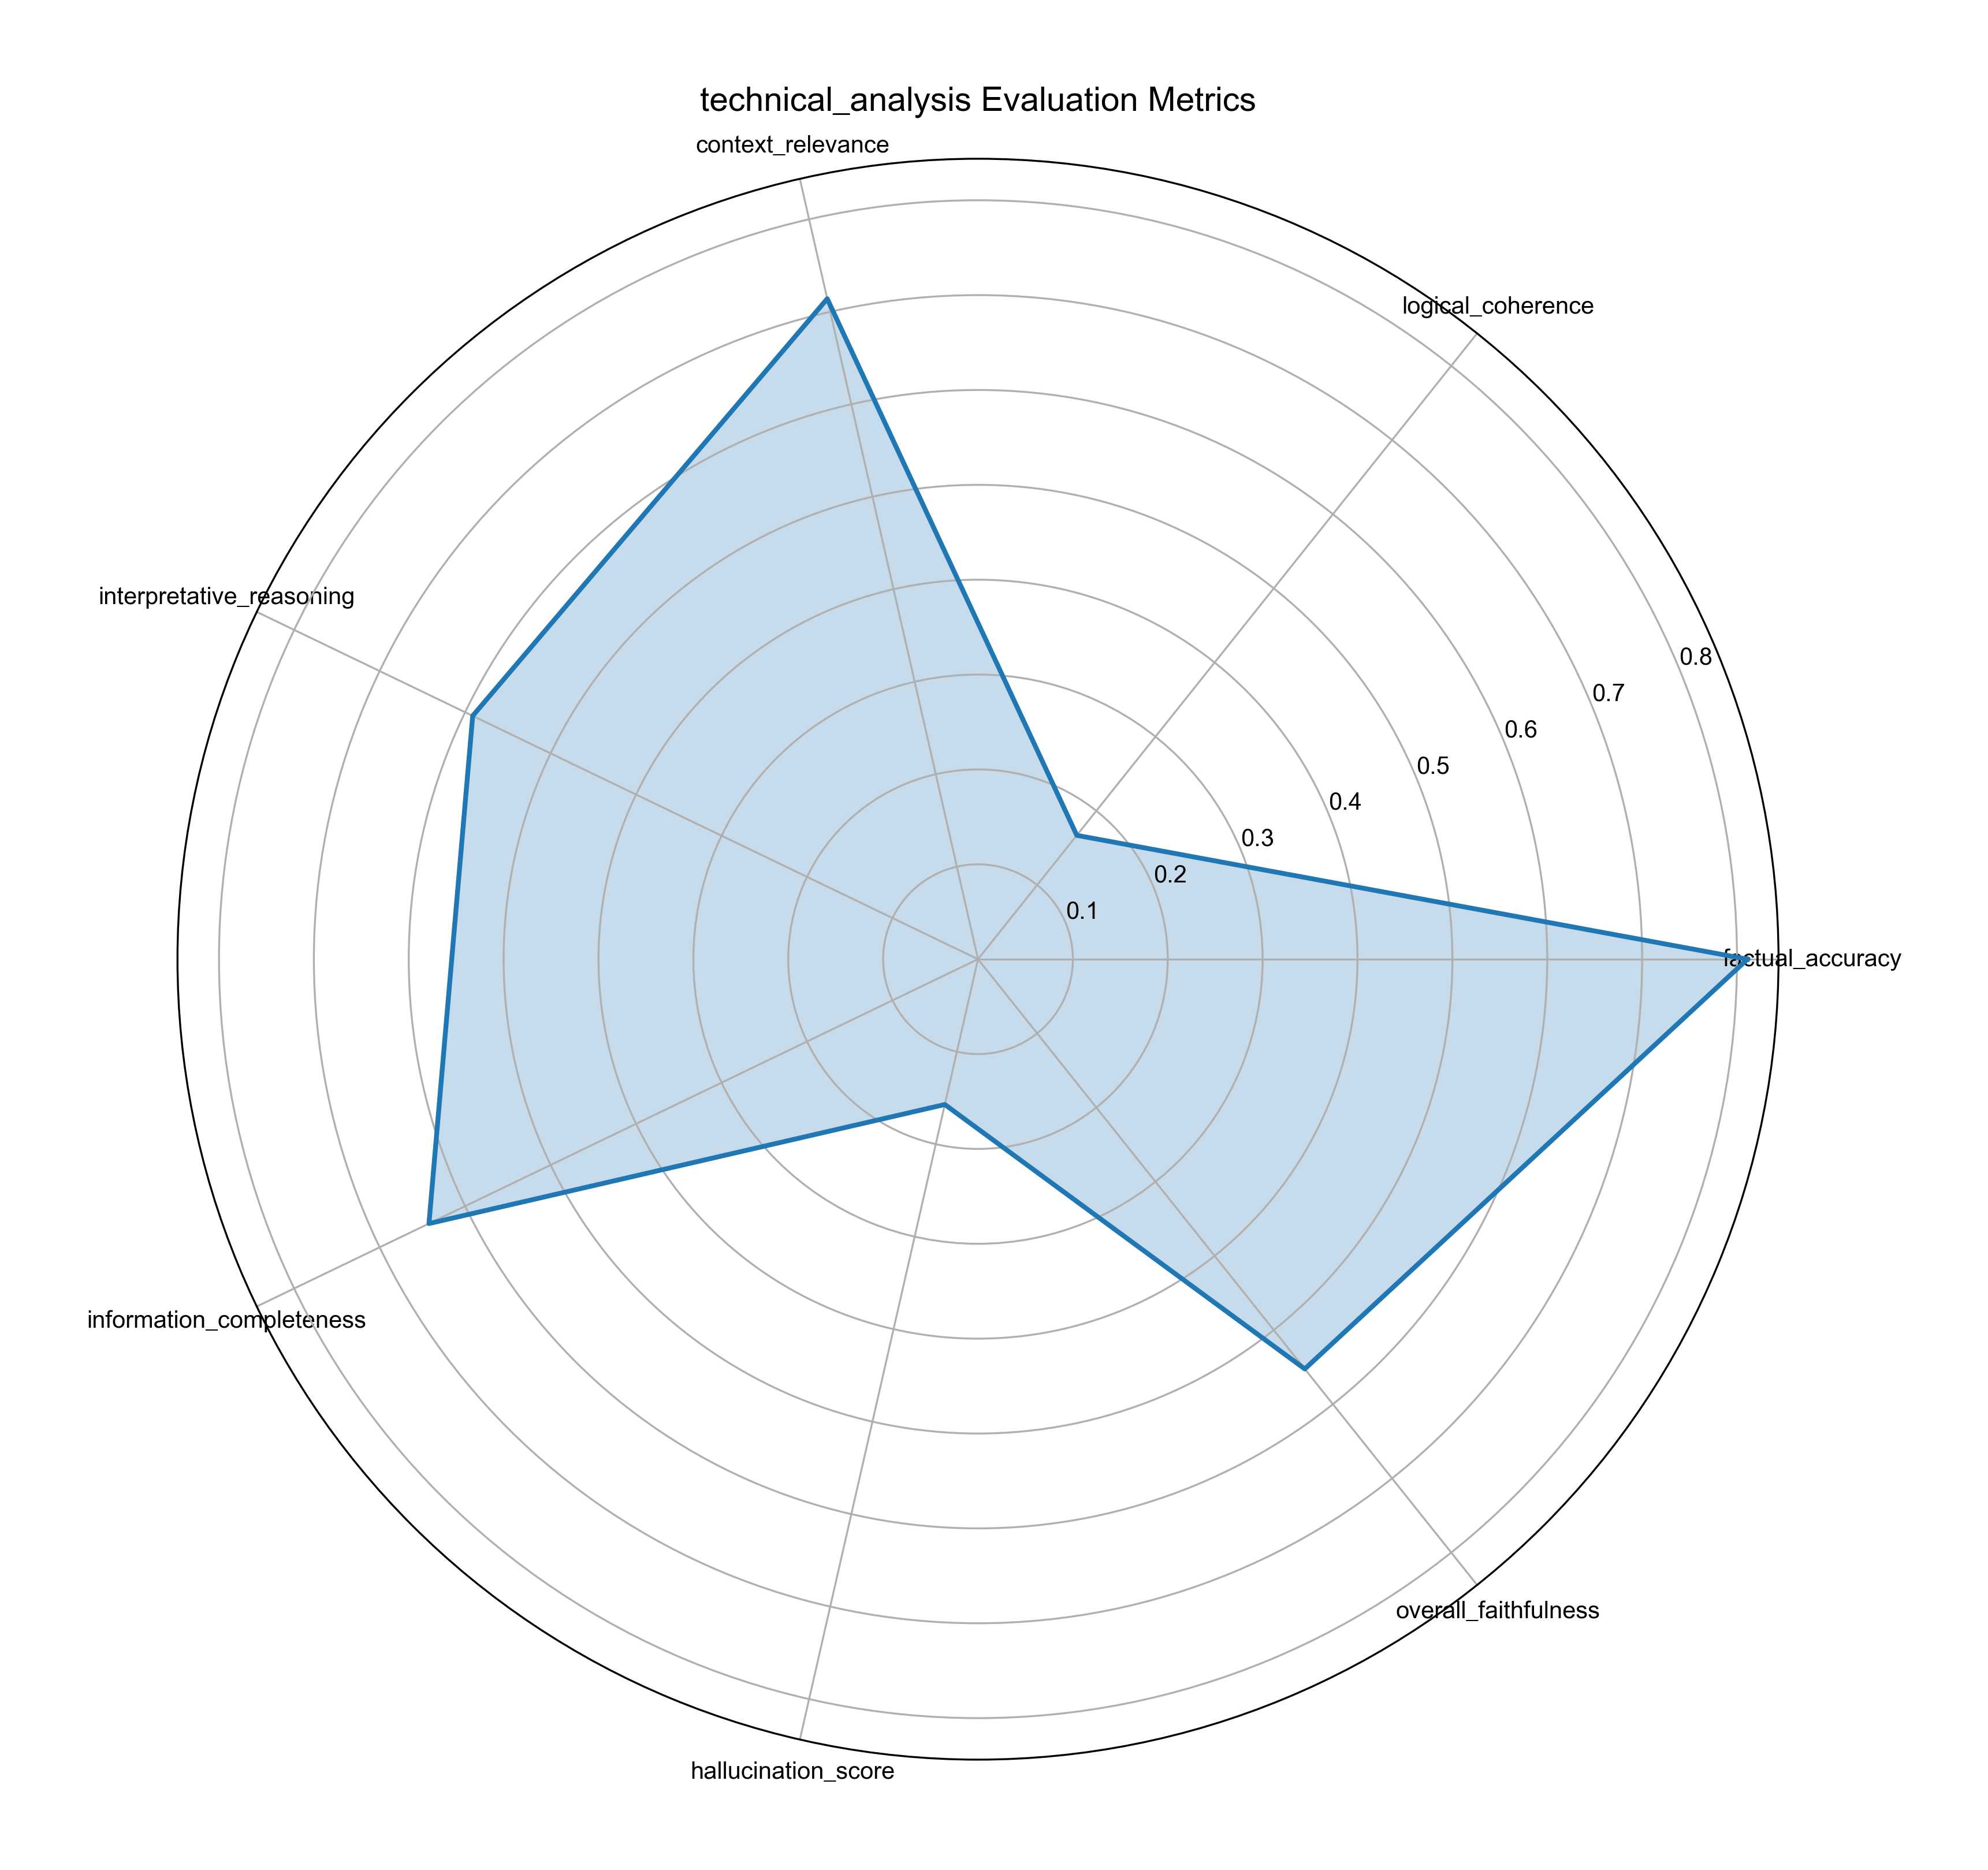
\includegraphics[width=0.6\textwidth]{figures/types/technical_analysis_radar_gpt-4.png}
\caption{Technical Analysis Performance Radar}
\label{fig:technical_radar}
\end{figure}

\textbf{Analysis}:
\begin{itemize}
    \item All models show improved performance in factual accuracy for technical content
    \item GPT-4 achieves the highest context relevance (0.7141), indicating better understanding of technical contexts
    \item Lower logical coherence scores suggest challenges in organizing technical information
\end{itemize}

\subsubsection{Medical Advice}
The medical advice evaluation assessed the models' ability to provide accurate and reliable health-related information.

\begin{table}[!htbp]
\centering
\setlength{\tabcolsep}{4pt}  % Reduce table column spacing
\begin{tabular}{|l|c|c|c|c|c|c|c|}
\hline
\textbf{Model} & \textbf{FA} & \textbf{LC} & \textbf{CR} & \textbf{IR} 
& \textbf{IC} & \textbf{HS} & \textbf{OF} \\
\hline
GPT-3.5-Turbo & 0.92 & 0.58 & 0.65 & 0.40 & 0.76 & 0.55 & 0.68 \\
GPT-4-Turbo & 0.80 & 0.35 & 0.61 & 0.52 & 0.82 & 0.32 & 0.66 \\
GPT-4 & 0.91 & 0.46 & 0.66 & 0.46 & 0.71 & 0.58 & 0.66 \\
\hline
\end{tabular}
\caption{Medical Advice Metrics}
\label{tab:results_medical_metrics}
\begin{flushleft}
\small
FA: Factual Accuracy, LC: Logical Coherence, CR: Context Relevance,\\
IR: Interpretative Reasoning, IC: Information Completeness, HS: Hallucination Score, OF: Overall Faithfulness
\end{flushleft}
\end{table}

\begin{figure}[!htbp]
\centering
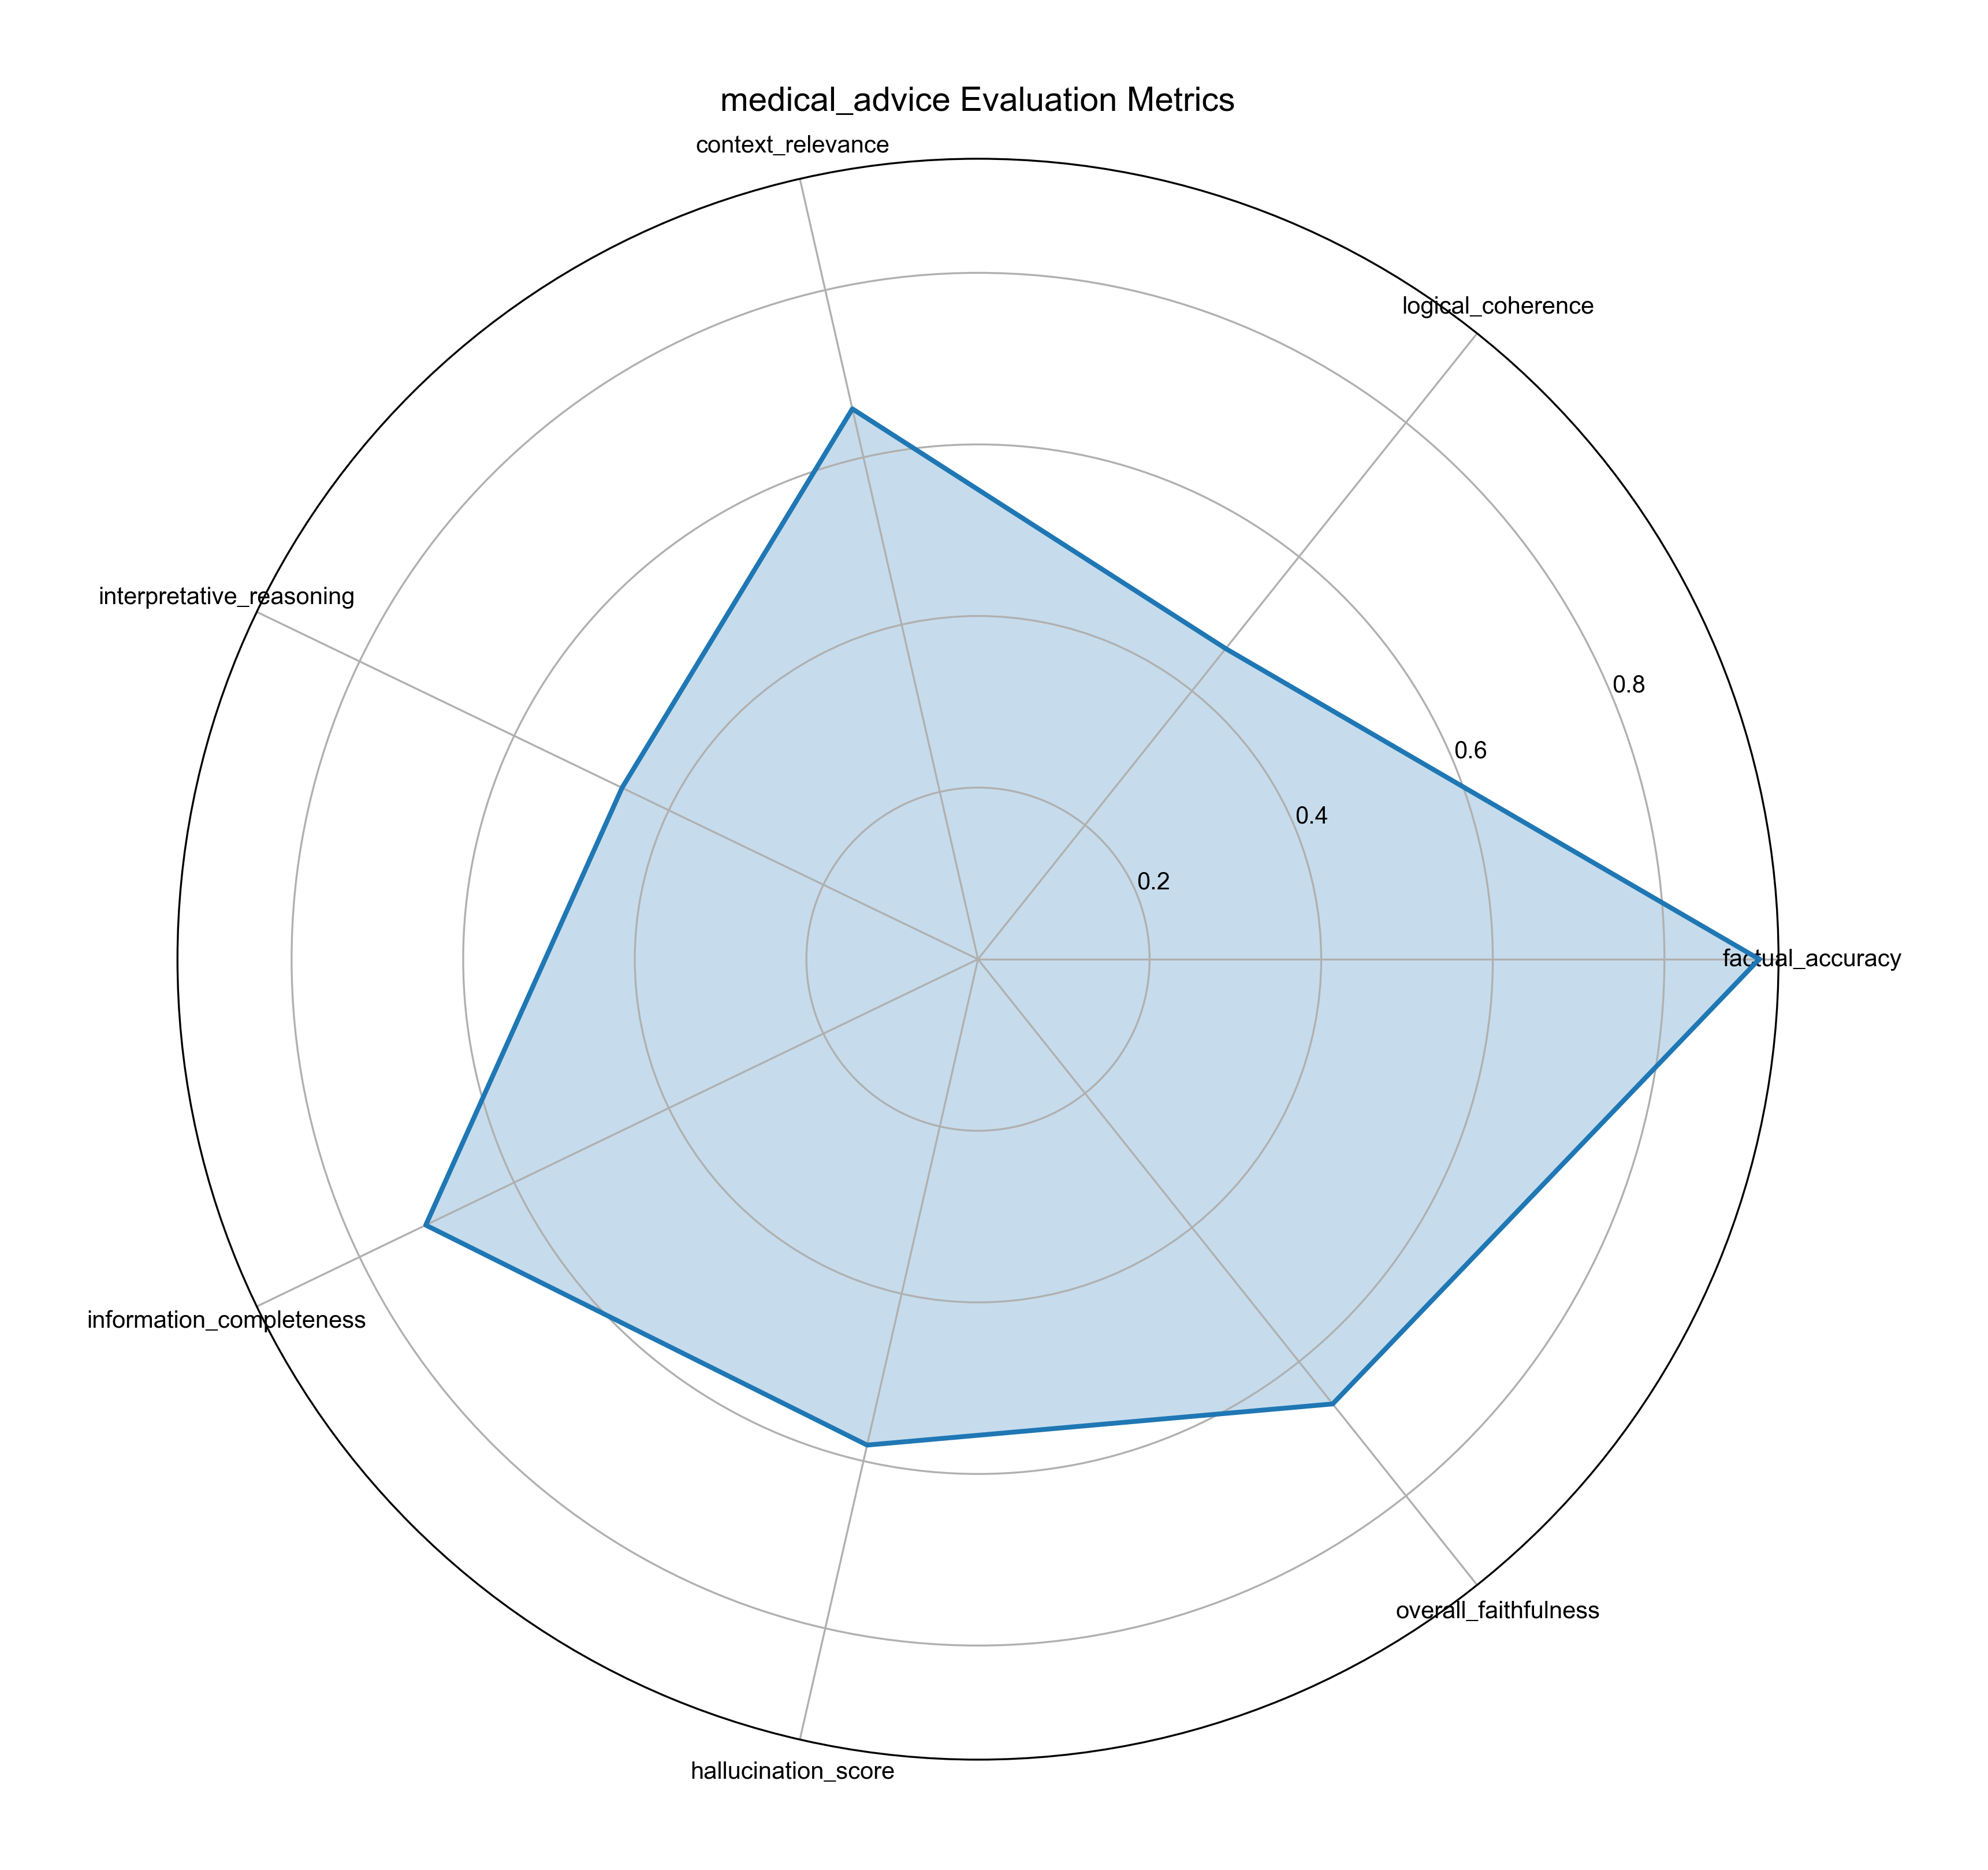
\includegraphics[width=0.6\textwidth]{figures/types/medical_advice_radar_gpt-4.png}
\caption{Medical Advice Performance Radar}
\label{fig:medical_radar}
\end{figure}

\textbf{Analysis}:
\begin{itemize}
    \item Notably high factual accuracy across all models, particularly in GPT-3.5-Turbo (0.9213)
    \item Strong information completeness scores reflect comprehensive medical responses
    \item Higher hallucination scores warrant attention in medical context
\end{itemize}

\subsubsection{Historical Analysis}
The historical analysis evaluation focused on the models' ability to accurately interpret and present historical information.

\begin{table}[!htbp]
\centering
\setlength{\tabcolsep}{4pt}  % Reduce table column spacing
\begin{tabular}{|l|c|c|c|c|c|c|c|}
\hline
\textbf{Model} & \textbf{FA} & \textbf{LC} & \textbf{CR} & \textbf{IR} 
& \textbf{IC} & \textbf{HS} & \textbf{OF} \\
\hline
GPT-3.5-Turbo & 0.82 & 0.17 & 0.70 & 0.59 & 0.79 & 0.11 & 0.56 \\
GPT-4-Turbo & 0.82 & 0.20 & 0.76 & 0.60 & 0.72 & 0.11 & 0.57 \\
GPT-4 & 0.82 & 0.20 & 0.76 & 0.60 & 0.72 & 0.11 & 0.57 \\
\hline
\end{tabular}
\caption{Historical Analysis Metrics}
\label{tab:results_historical_metrics}
\begin{flushleft}
\small
FA: Factual Accuracy, LC: Logical Coherence, CR: Context Relevance,\\
IR: Interpretative Reasoning, IC: Information Completeness, HS: Hallucination Score, OF: Overall Faithfulness
\end{flushleft}
\end{table}

\begin{figure}[!htbp]
\centering
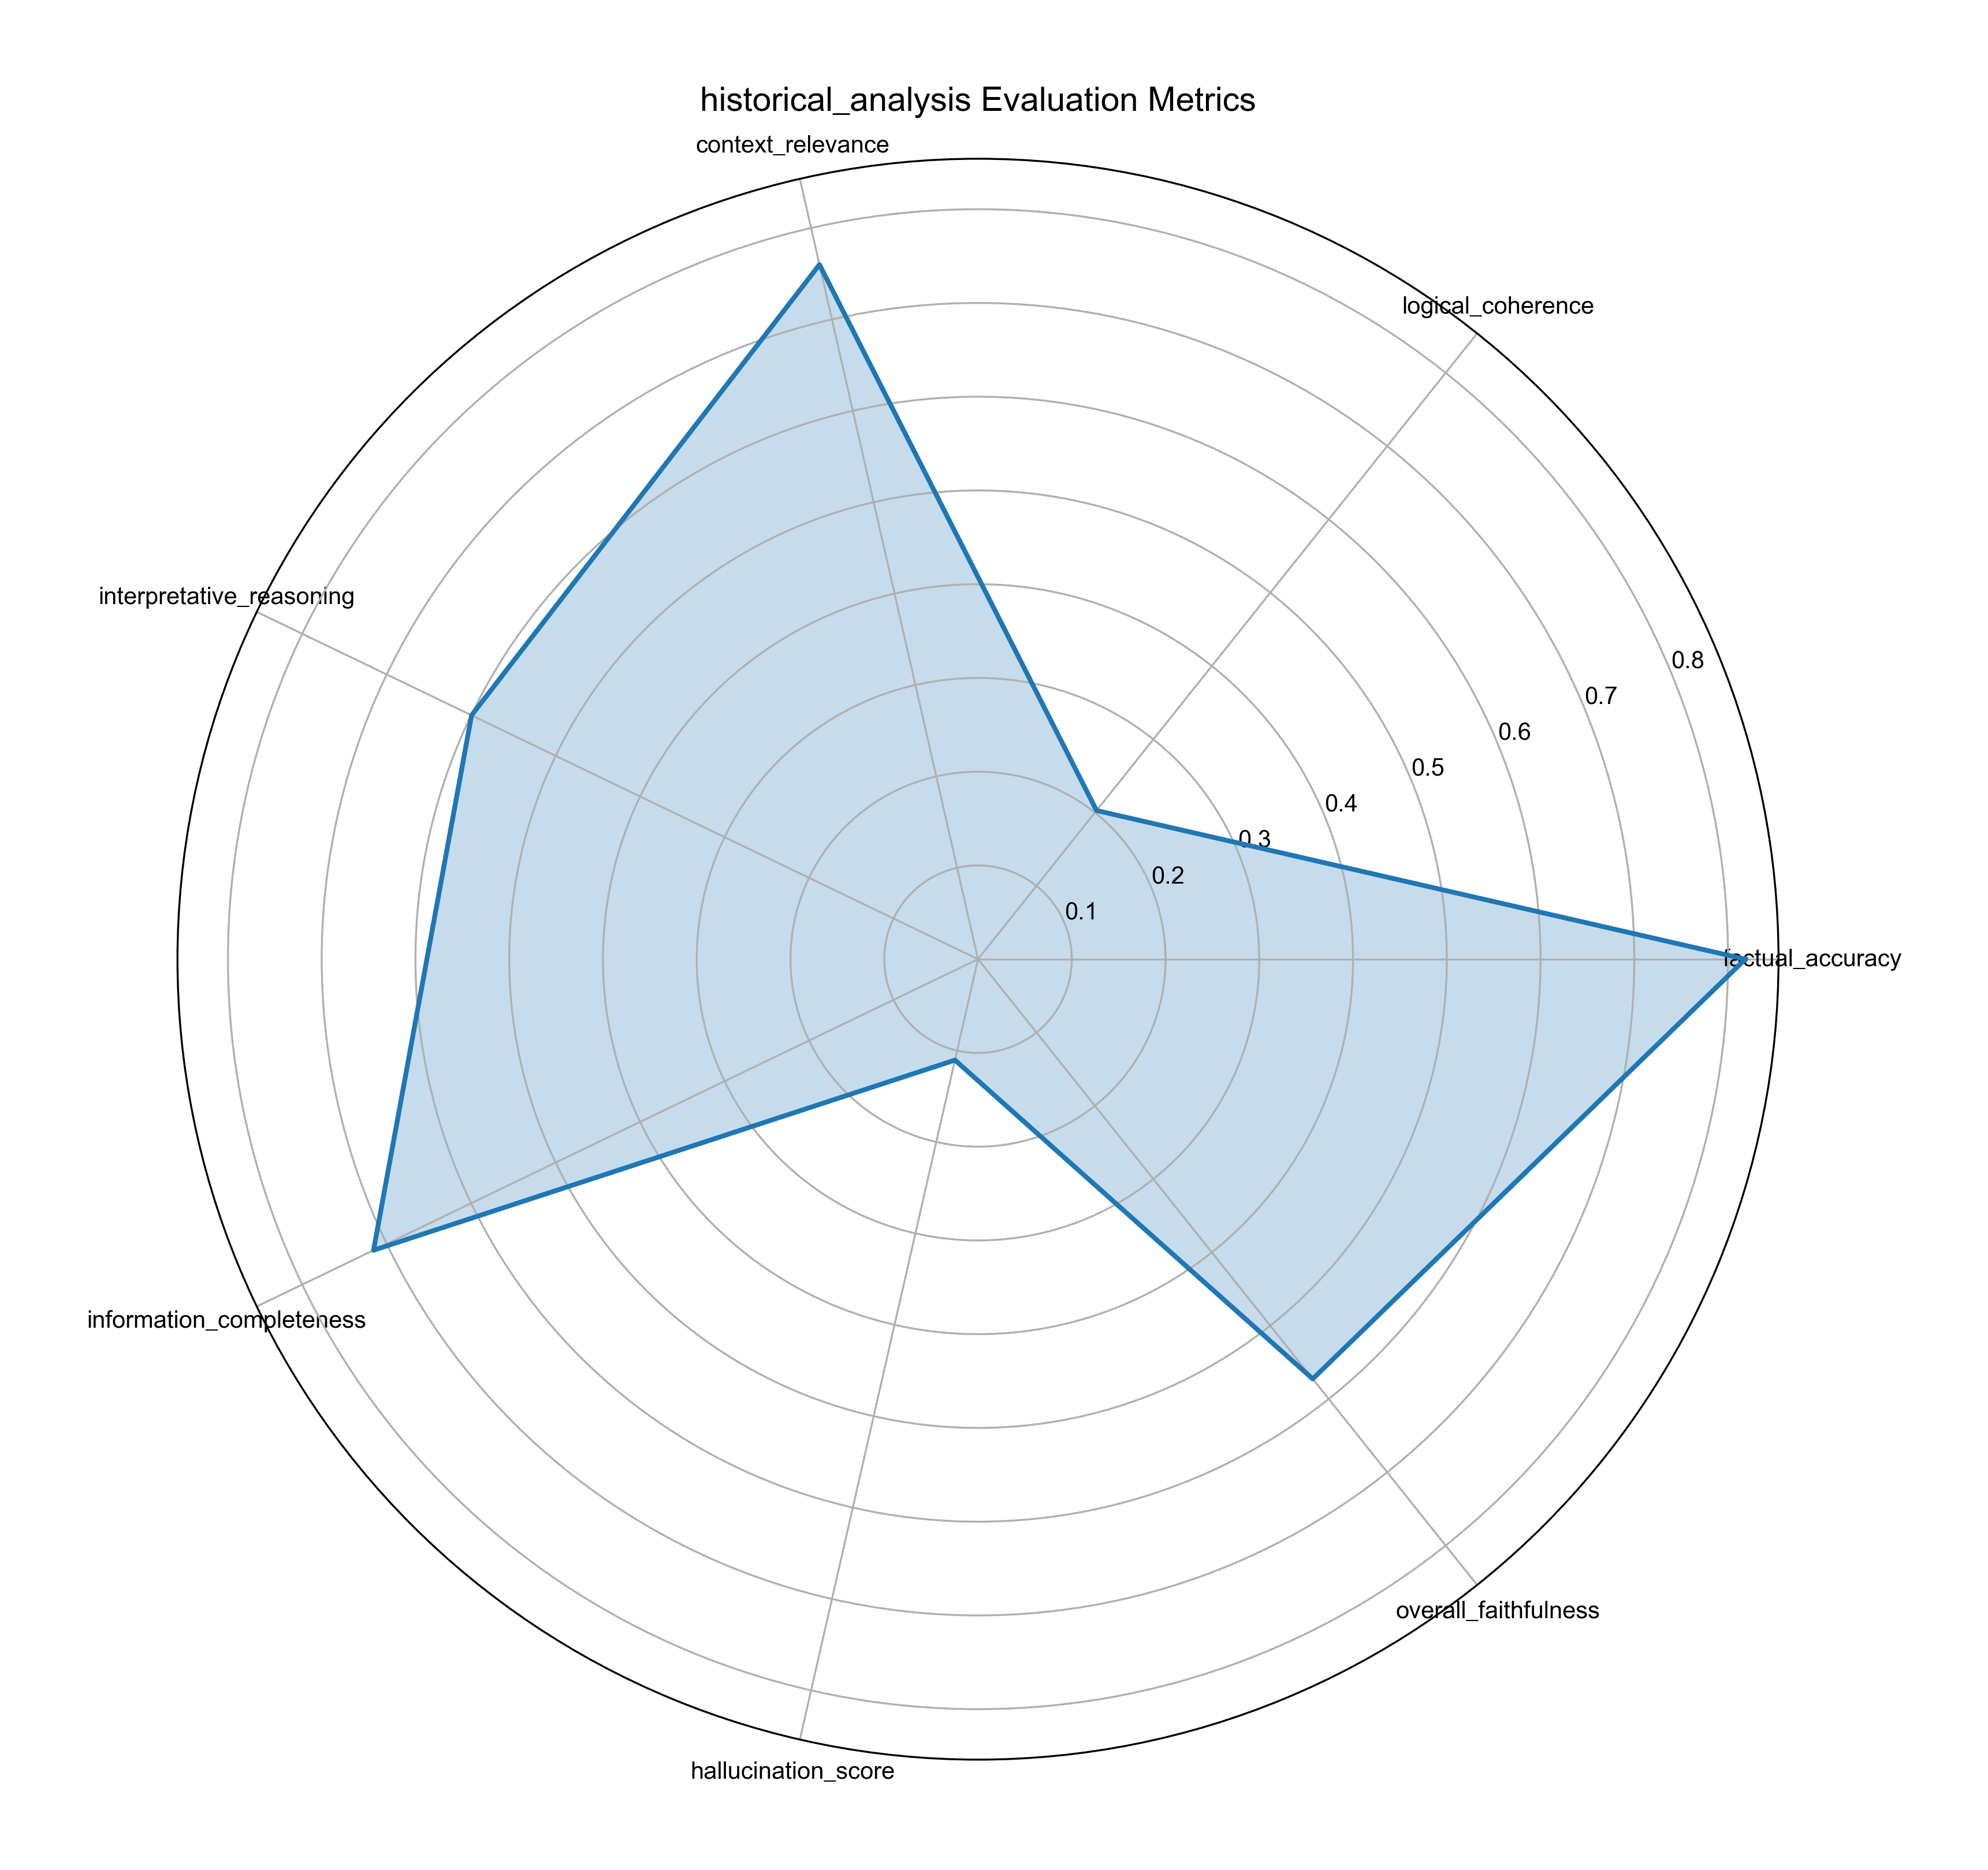
\includegraphics[width=0.6\textwidth]{figures/types/historical_analysis_radar_gpt-4.png}
\caption{Historical Analysis Performance Radar}
\label{fig:historical_radar}
\end{figure}

\textbf{Analysis}:
\begin{itemize}
    \item All models demonstrate consistent factual accuracy (0.82) in historical content
    \item Strong context relevance scores (>0.70) indicate good historical context understanding
    \item Lower logical coherence scores suggest challenges in organizing historical narratives
    \item Notably low hallucination scores (0.11) indicate reliable historical information presentation
\end{itemize}

\subsubsection{Current Events}
The current events evaluation assessed the models' ability to handle contemporary information and recent developments.

\begin{table}[!htbp]
\centering
\setlength{\tabcolsep}{4pt}  % Reduce table column spacing
\begin{tabular}{|l|c|c|c|c|c|c|c|}
\hline
\textbf{Model} & \textbf{FA} & \textbf{LC} & \textbf{CR} & \textbf{IR} 
& \textbf{IC} & \textbf{HS} & \textbf{OF} \\
\hline
GPT-3.5-Turbo & 0.80 & 0.52 & 0.43 & 0.54 & 0.66 & 0.51 & 0.61 \\
GPT-4-Turbo & 0.76 & 0.39 & 0.44 & 0.66 & 0.67 & 0.33 & 0.59 \\
GPT-4 & 0.78 & 0.45 & 0.44 & 0.66 & 0.67 & 0.33 & 0.59 \\
\hline
\end{tabular}
\caption{Current Events Metrics}
\label{tab:results_current_events_metrics}
\begin{flushleft}
\small
FA: Factual Accuracy, LC: Logical Coherence, CR: Context Relevance,\\
IR: Interpretative Reasoning, IC: Information Completeness, HS: Hallucination Score, OF: Overall Faithfulness
\end{flushleft}
\end{table}

\begin{figure}[!htbp]
\centering
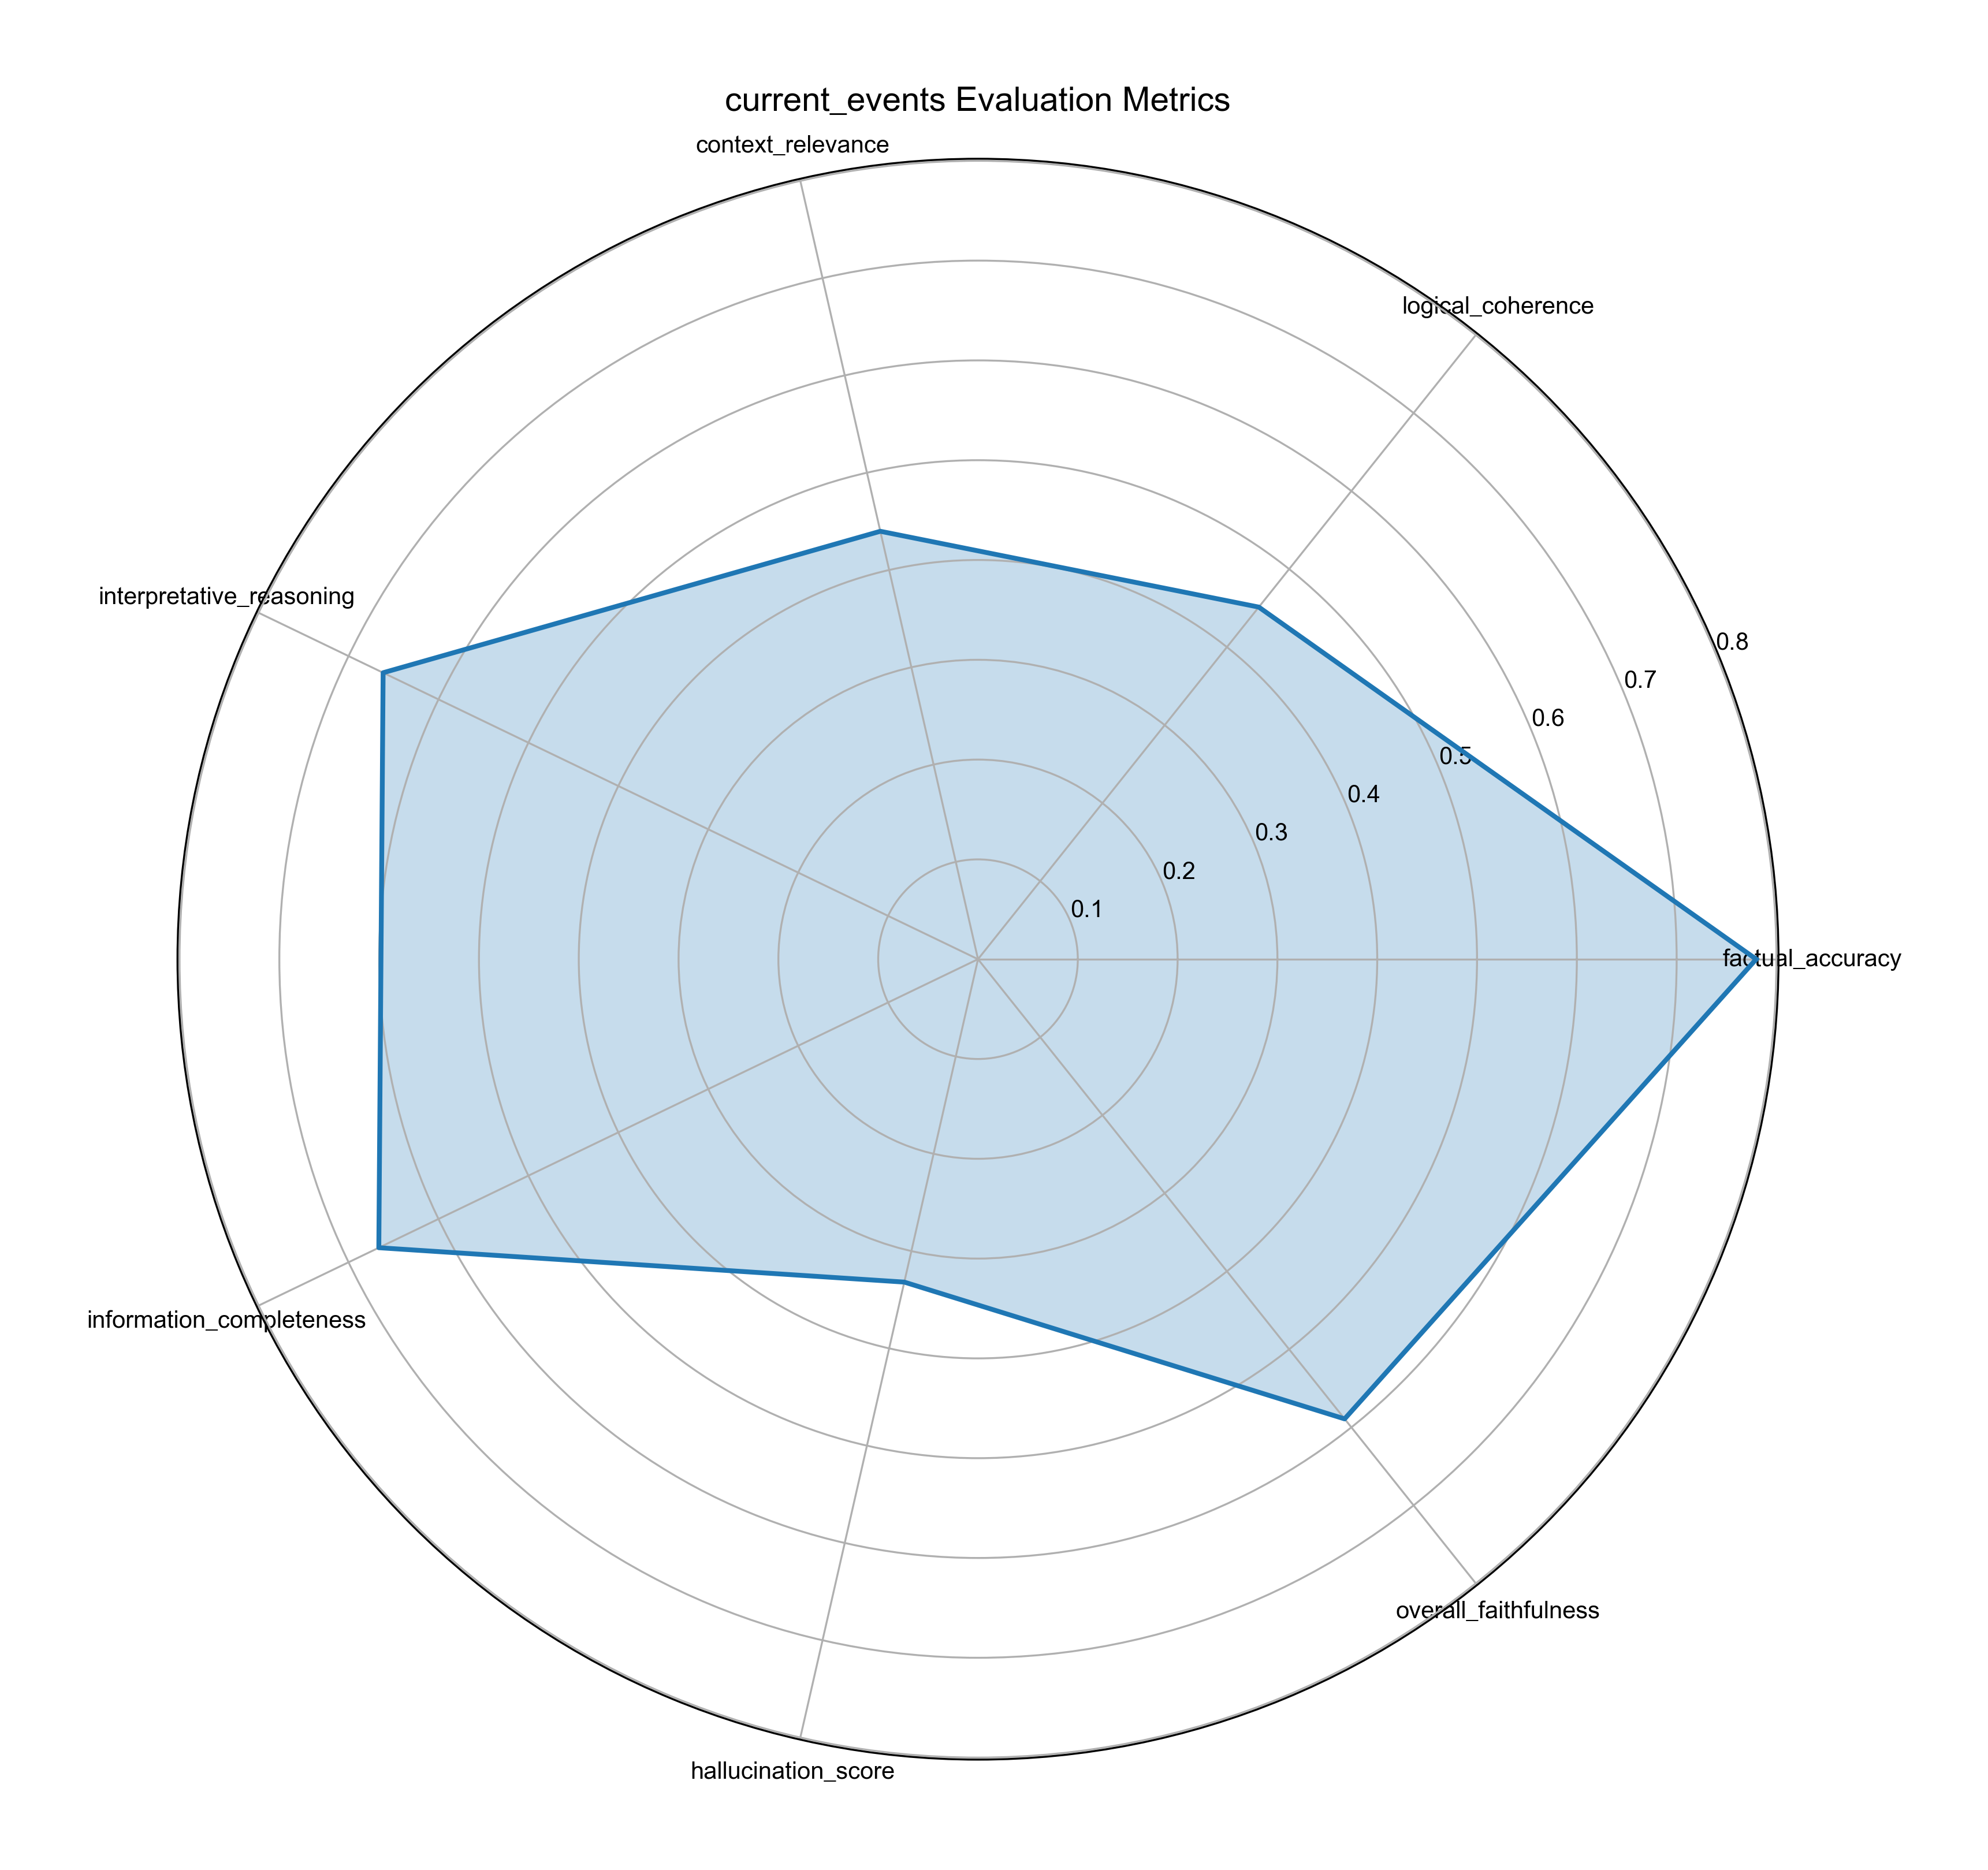
\includegraphics[width=0.6\textwidth]{figures/types/current_events_radar_gpt-4.png}
\caption{Current Events Performance Radar}
\label{fig:current_events_radar}
\end{figure}

\textbf{Analysis}:
\begin{itemize}
    \item GPT-3.5-Turbo shows highest factual accuracy (0.80) in current events
    \item Lower context relevance scores (<0.45) suggest challenges in connecting contemporary information
    \item Higher hallucination scores indicate increased uncertainty in recent event analysis
    \item Strong interpretative reasoning in GPT-4 variants (0.66) shows good analytical capabilities
\end{itemize}

\subsubsection{Sample Type Comparison}
A comprehensive comparison across different sample types reveals how models adapt to varying content domains.

\begin{figure}[!htbp]
\centering
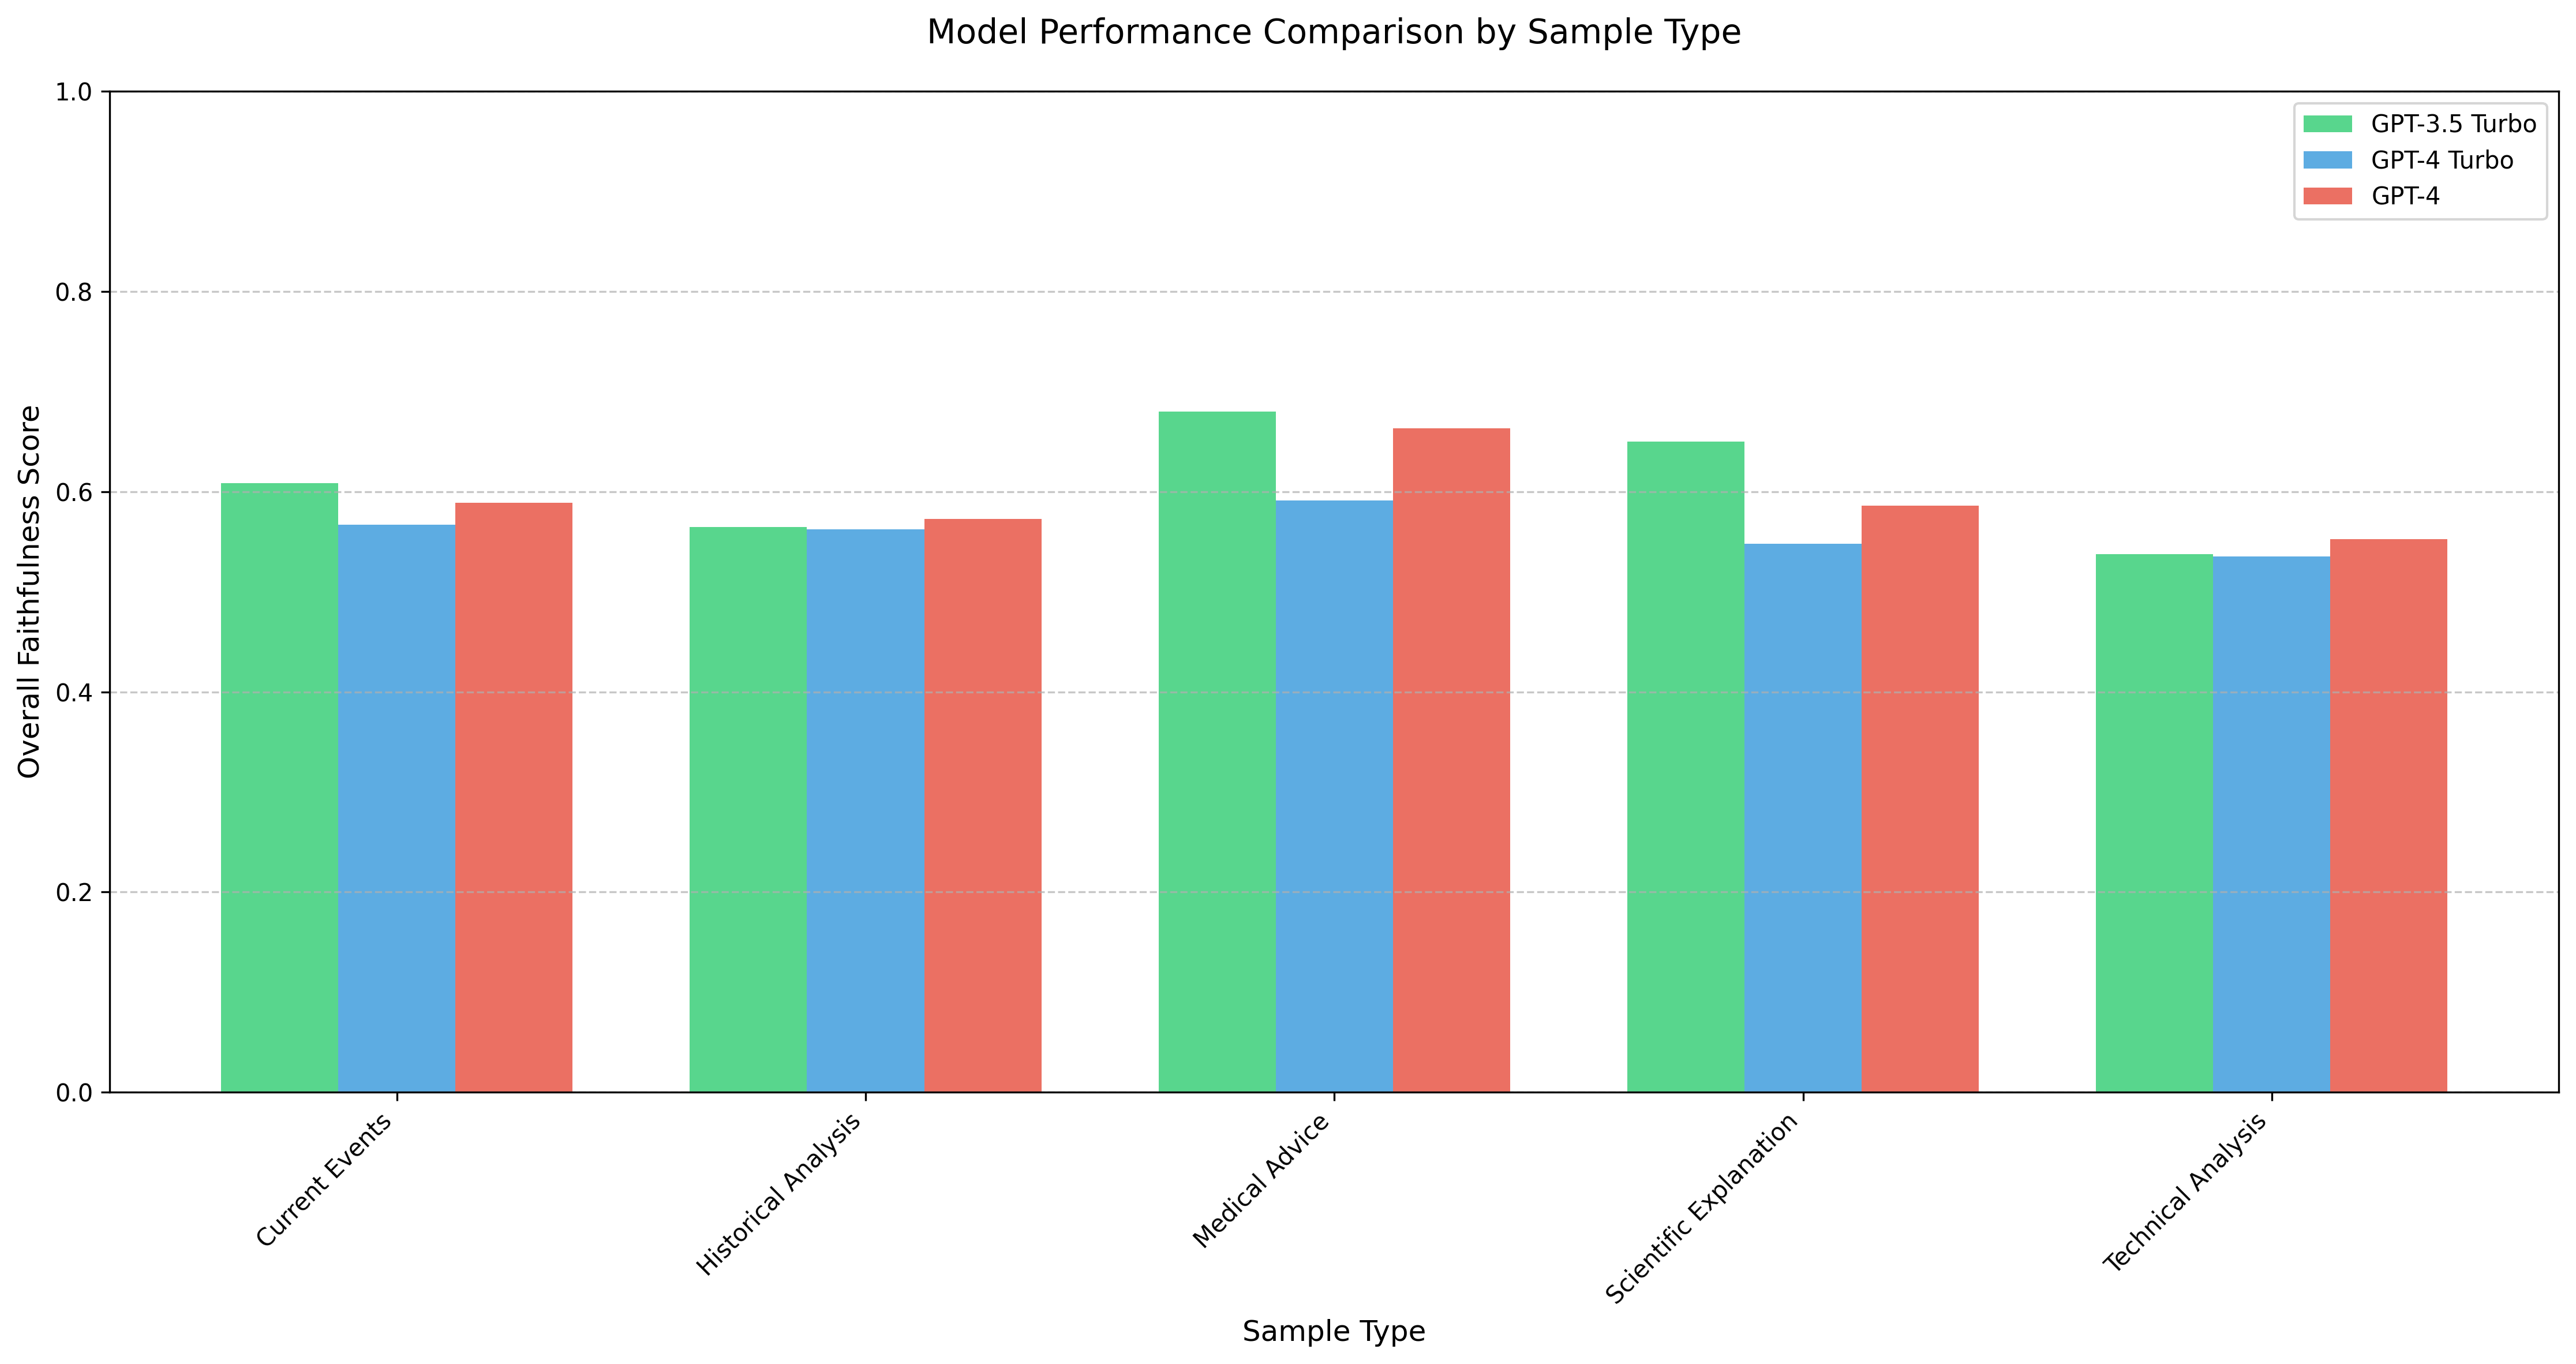
\includegraphics[width=0.8\textwidth]{figures/types/type_comparison.png}
\caption{Performance Comparison Across Sample Types}
\label{fig:type_comparison}
\end{figure}

\textbf{Cross-Type Analysis}:
\begin{itemize}
    \item Different content types present unique challenges for each model
    \item Performance patterns vary significantly across domains
    \item Some metrics show consistent trends regardless of content type
\end{itemize}

\subsection{Visualization Analysis}

\subsubsection{Metric Distribution Analysis}
The box plots provide insights into the statistical distribution and variability of each metric across models.

\begin{figure}[!htbp]
\centering
\begin{subfigure}[b]{0.32\textwidth}
    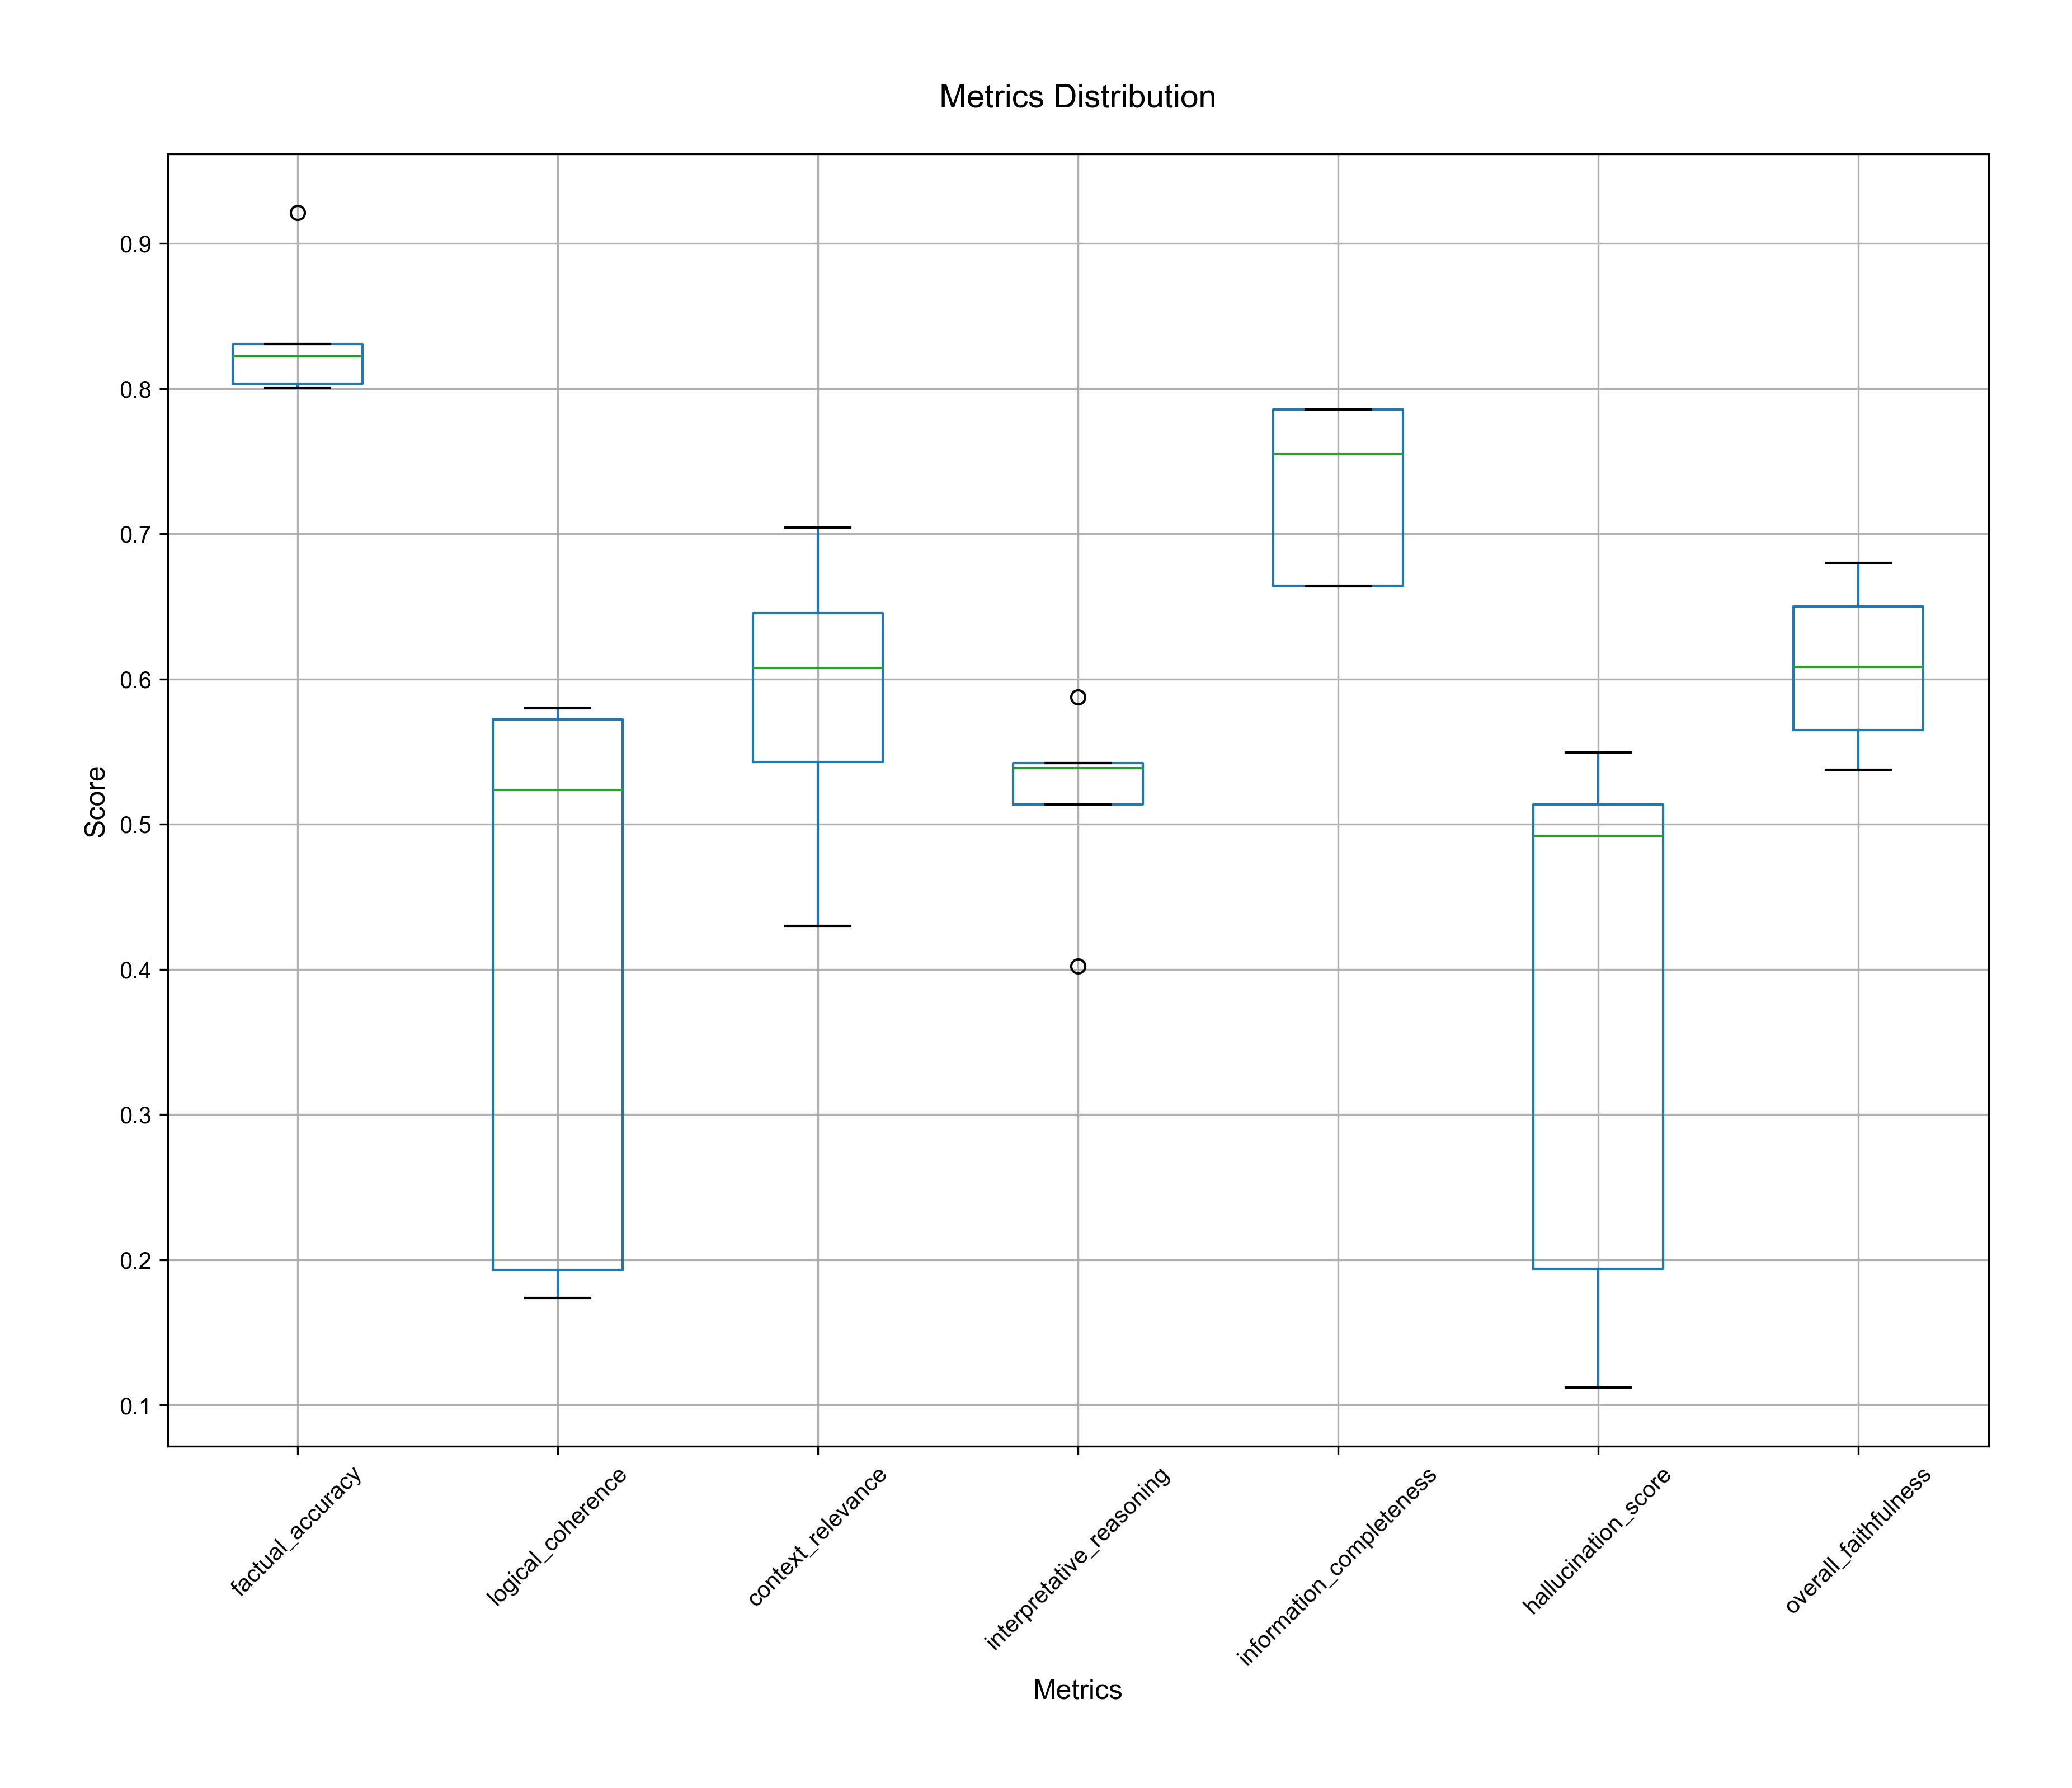
\includegraphics[width=\textwidth]{figures/visualization/metrics_boxplot_gpt-3.5-turbo.png}
    \caption{GPT-3.5-Turbo}
    \label{fig:metrics_boxplot_gpt35}
\end{subfigure}
\hfill
\begin{subfigure}[b]{0.32\textwidth}
    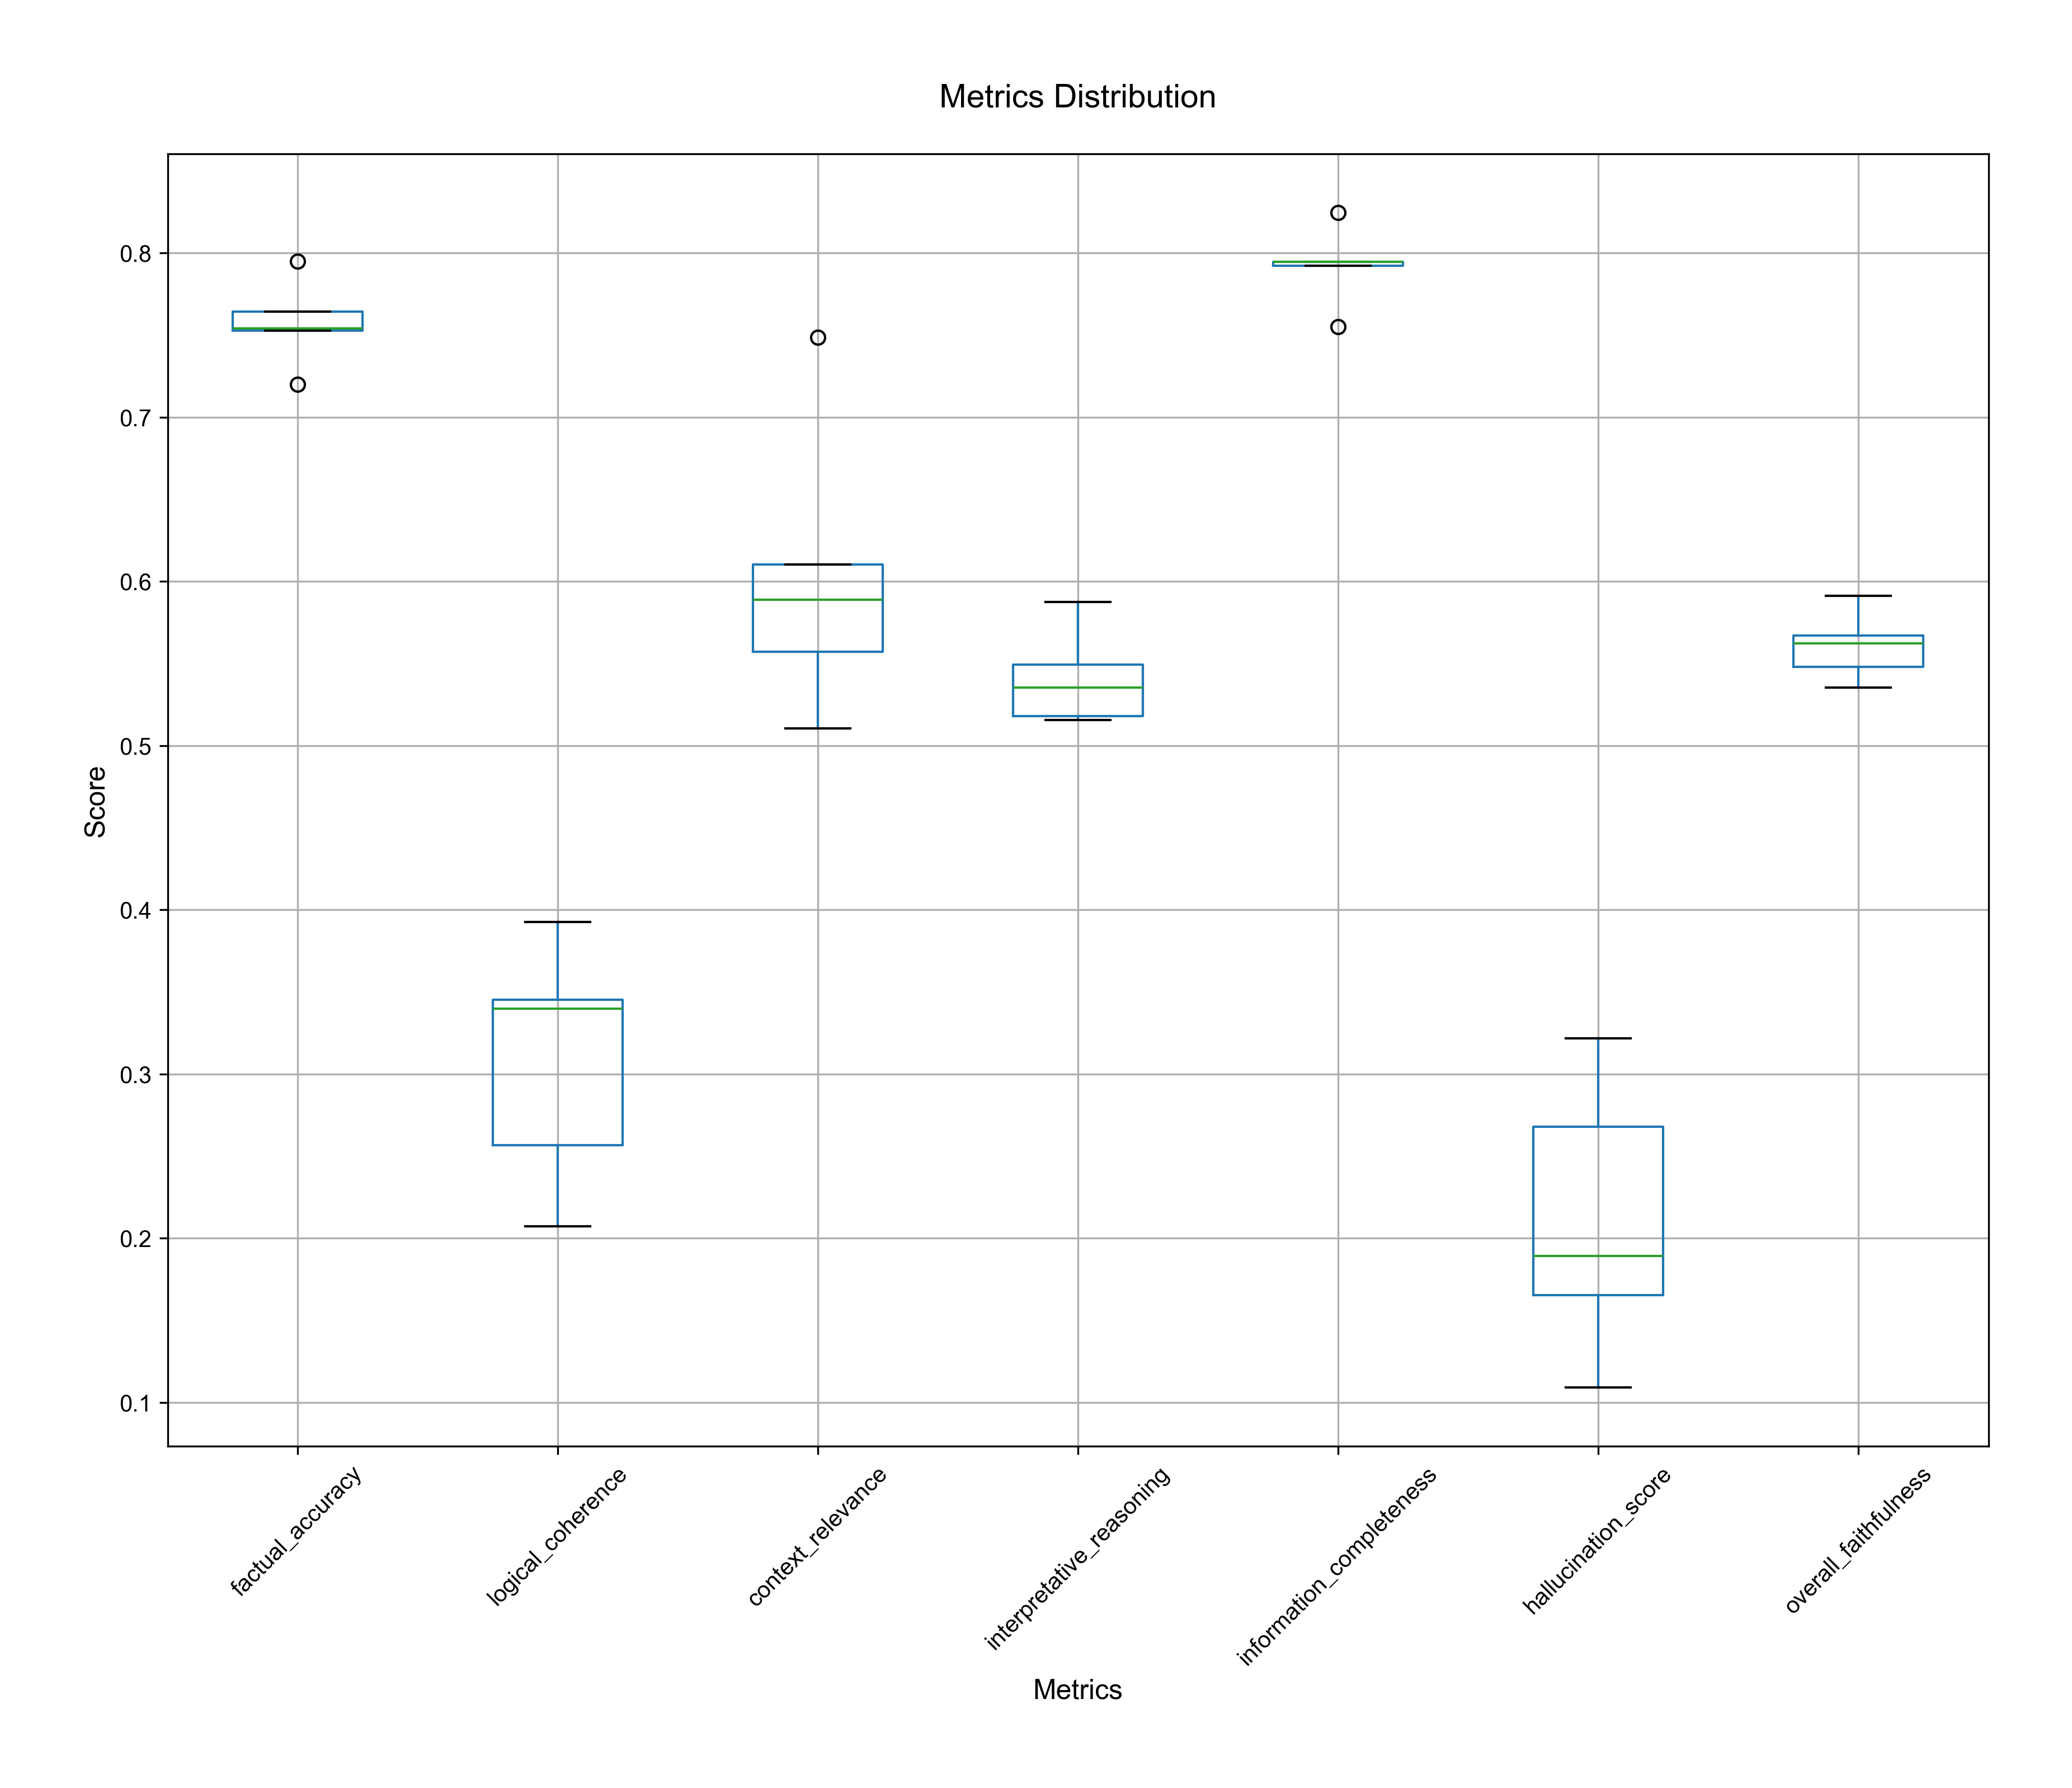
\includegraphics[width=\textwidth]{figures/visualization/metrics_boxplot_gpt-4-turbo.png}
    \caption{GPT-4-Turbo}
    \label{fig:metrics_boxplot_gpt4t}
\end{subfigure}
\hfill
\begin{subfigure}[b]{0.32\textwidth}
    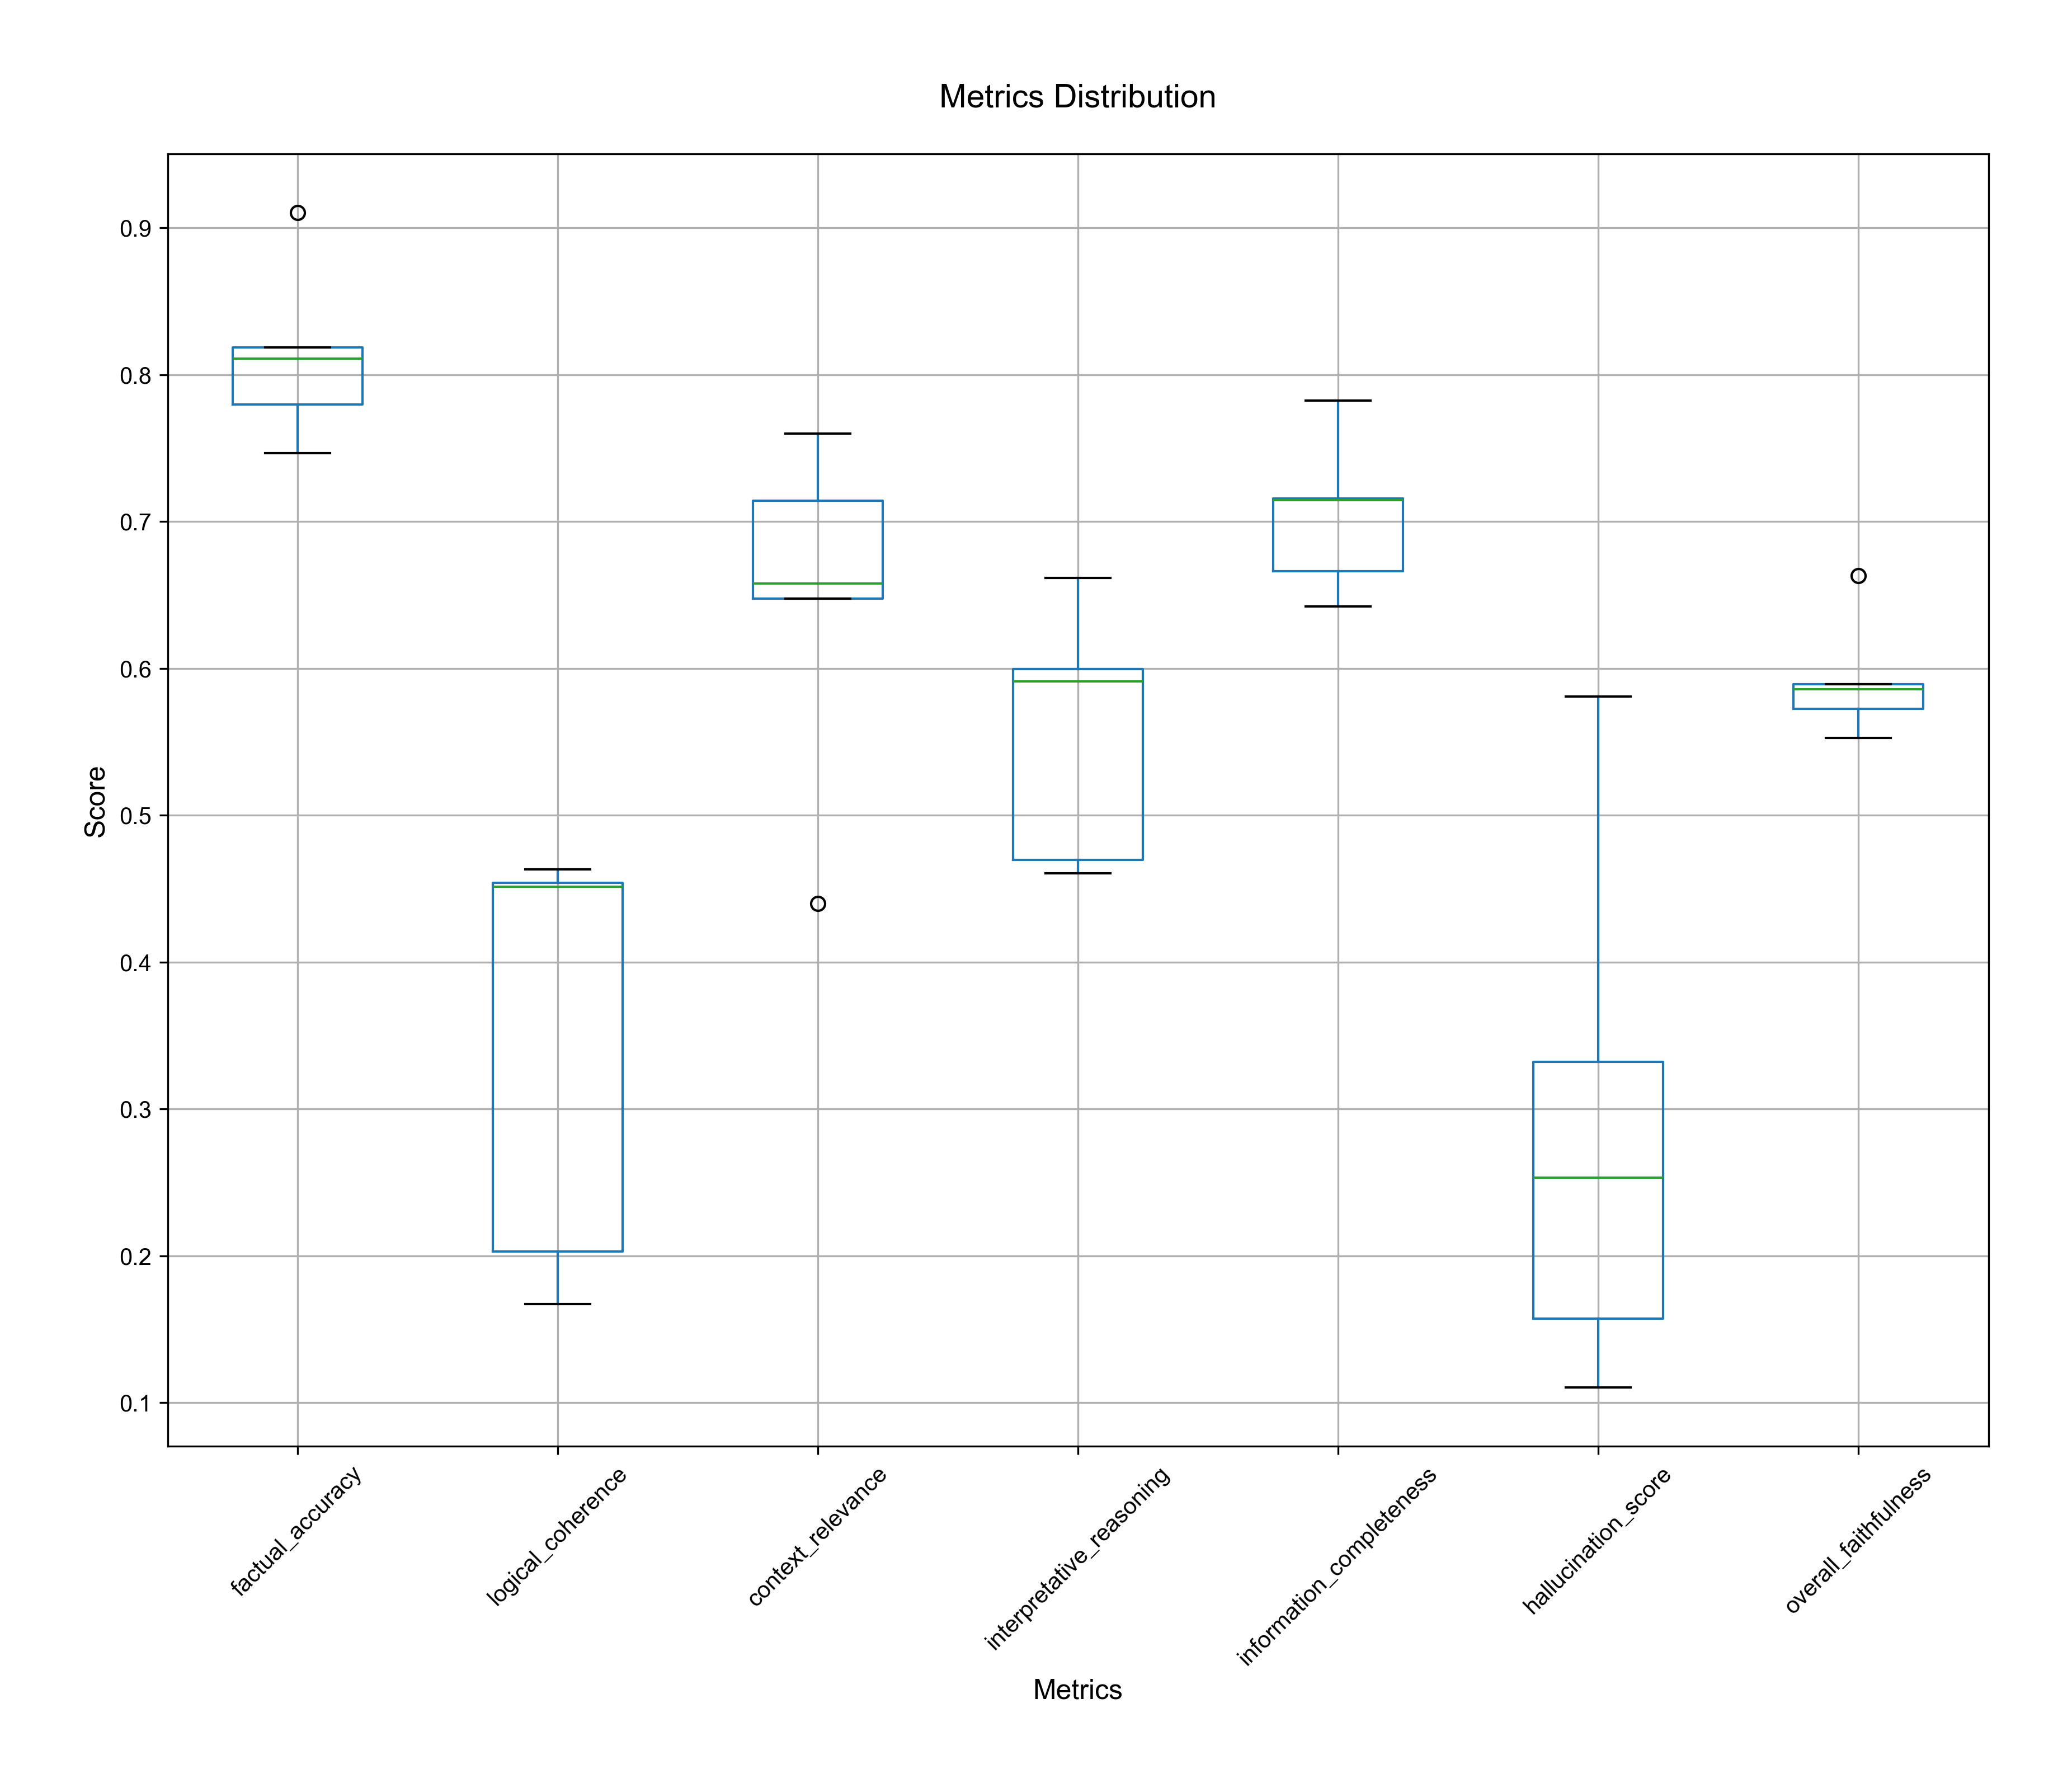
\includegraphics[width=\textwidth]{figures/visualization/metrics_boxplot_gpt-4.png}
    \caption{GPT-4}
    \label{fig:metrics_boxplot_gpt4}
\end{subfigure}
\caption{Metric Score Distributions by Model}
\label{fig:metrics_boxplots}
\end{figure}

\textbf{Distribution Insights}:
\begin{itemize}
    \item Factual accuracy shows the most consistent distribution across models
    \item Logical coherence exhibits the widest range of scores
    \item Hallucination scores show significant outliers, particularly in GPT-3.5-Turbo
\end{itemize}

\subsubsection{Correlation Analysis}
Heat maps visualize the relationships between different metrics, revealing important patterns and dependencies.

\begin{figure}[!htbp]
\centering
\begin{subfigure}[b]{0.32\textwidth}
    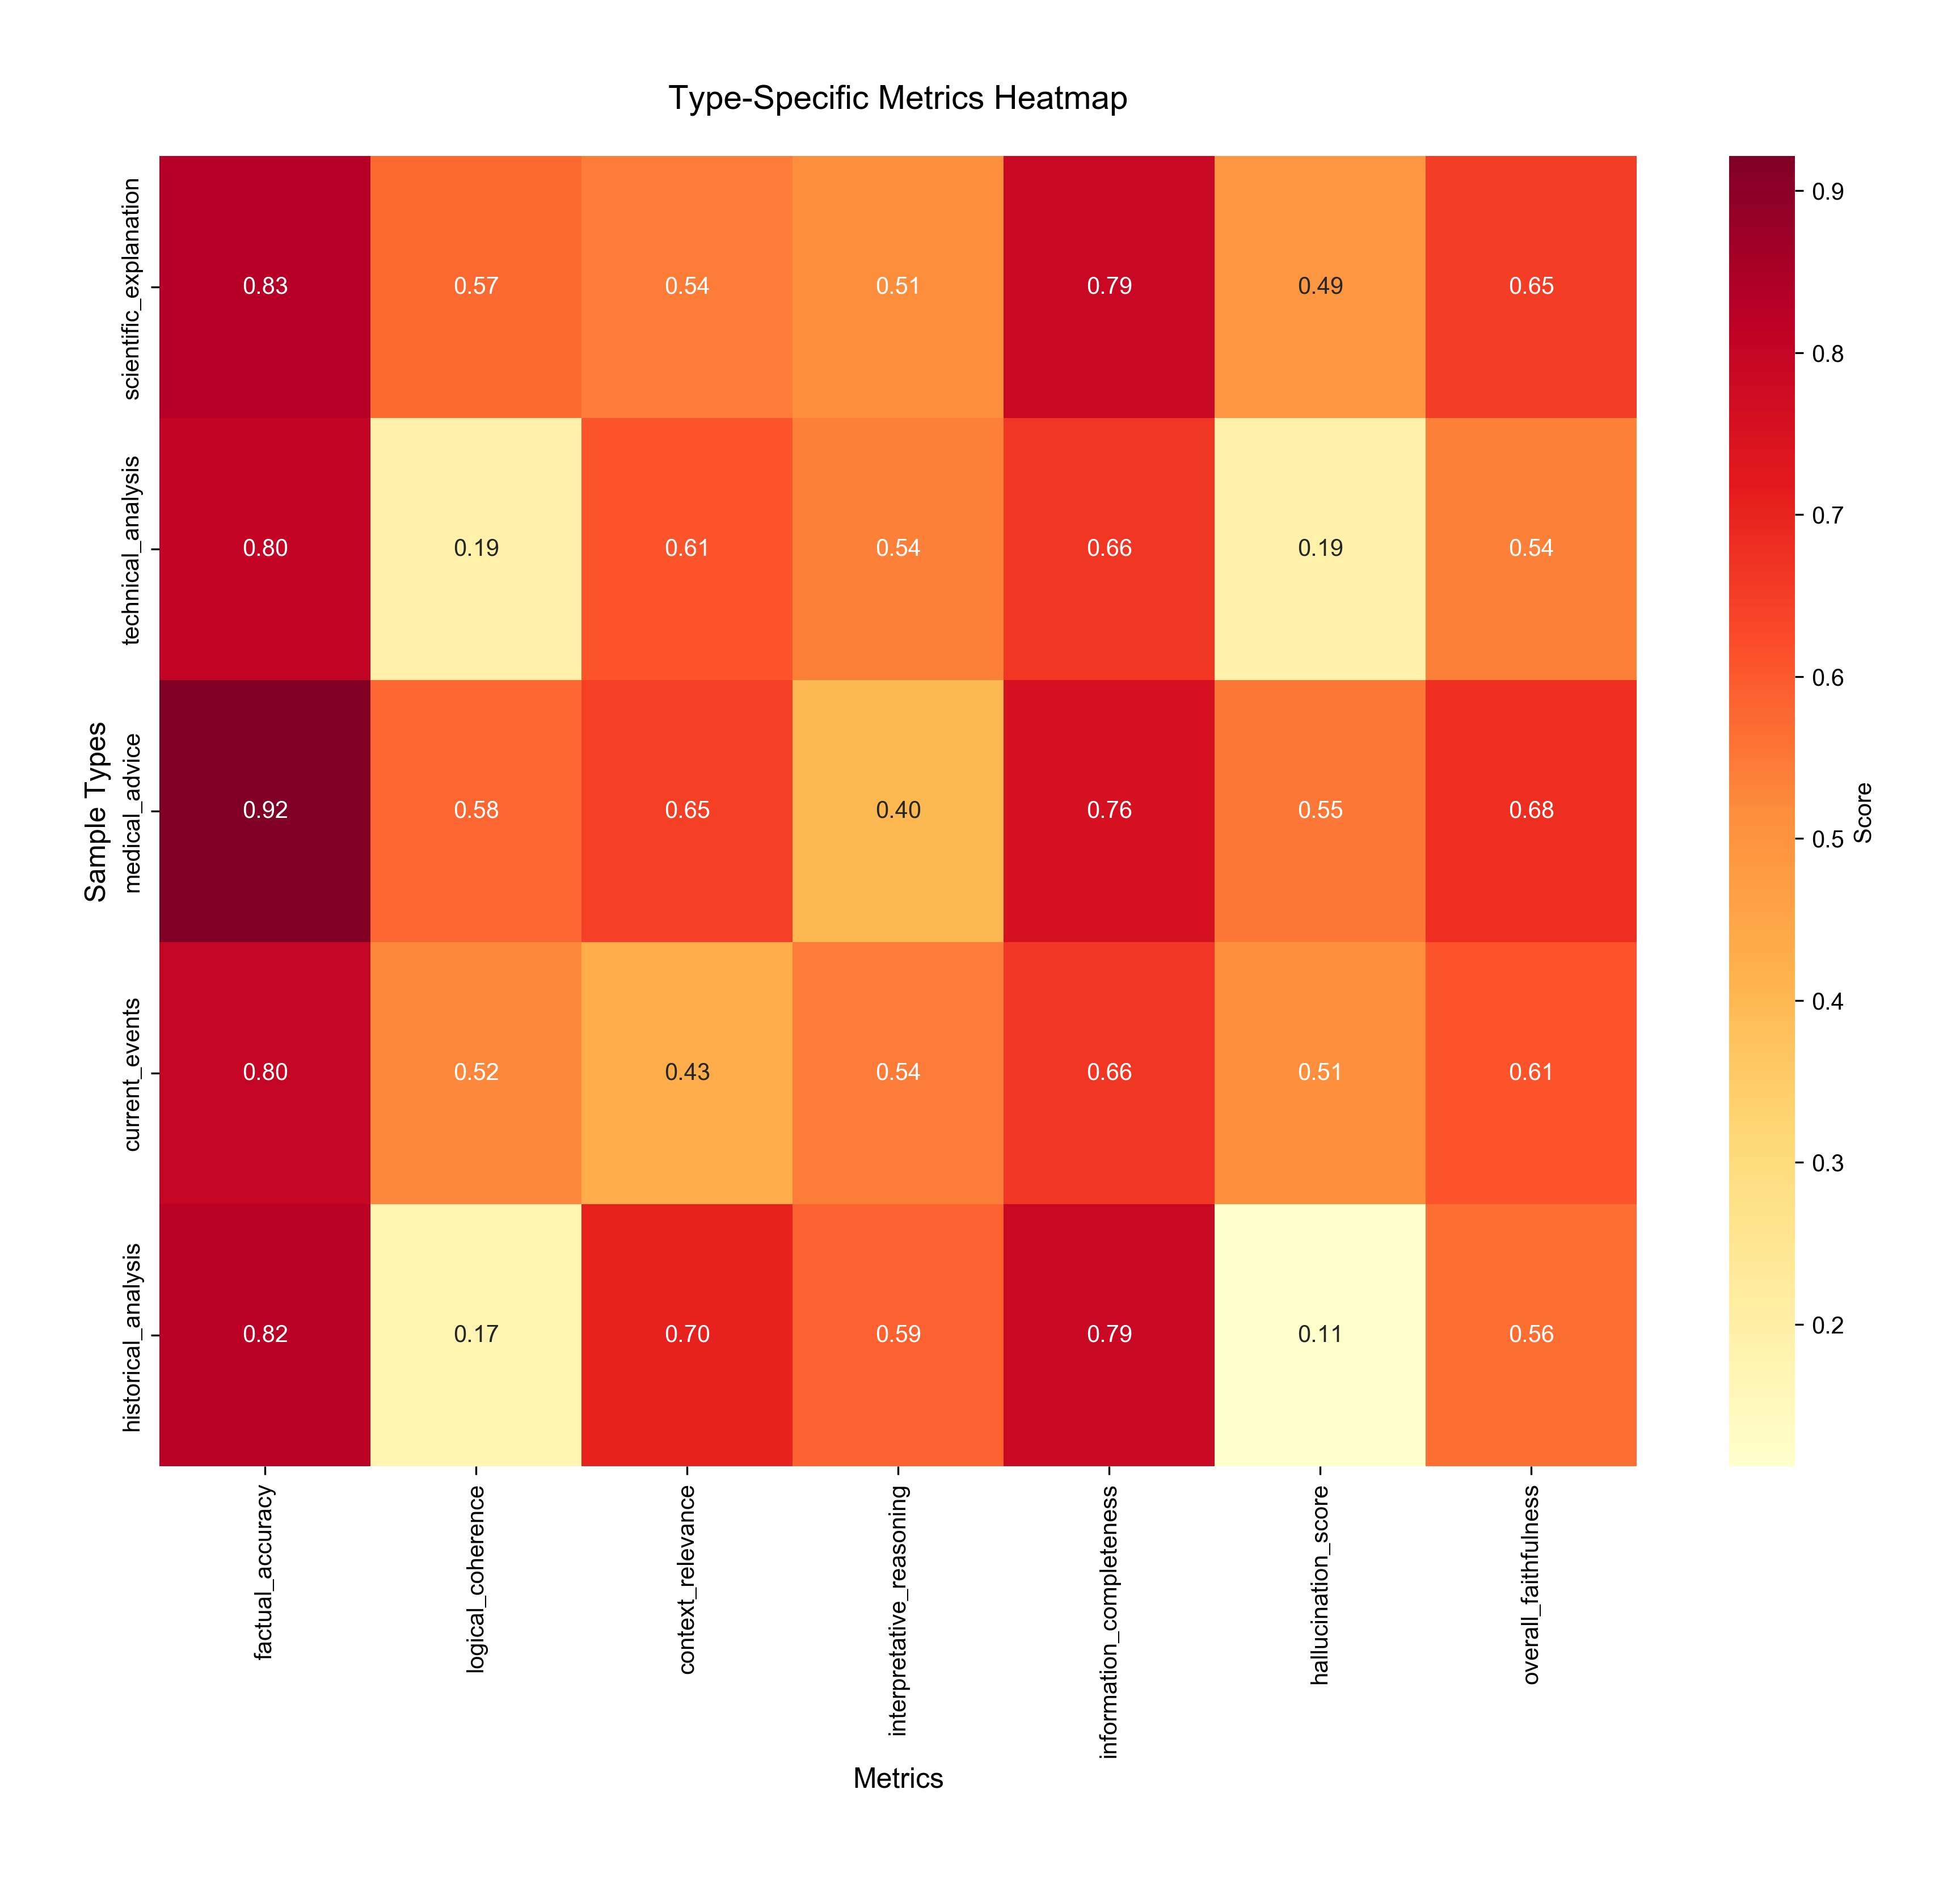
\includegraphics[width=\textwidth]{figures/visualization/metrics_heatmap_gpt-3.5-turbo.png}
    \caption{GPT-3.5-Turbo}
    \label{fig:metrics_heatmap_gpt35}
\end{subfigure}
\hfill
\begin{subfigure}[b]{0.32\textwidth}
    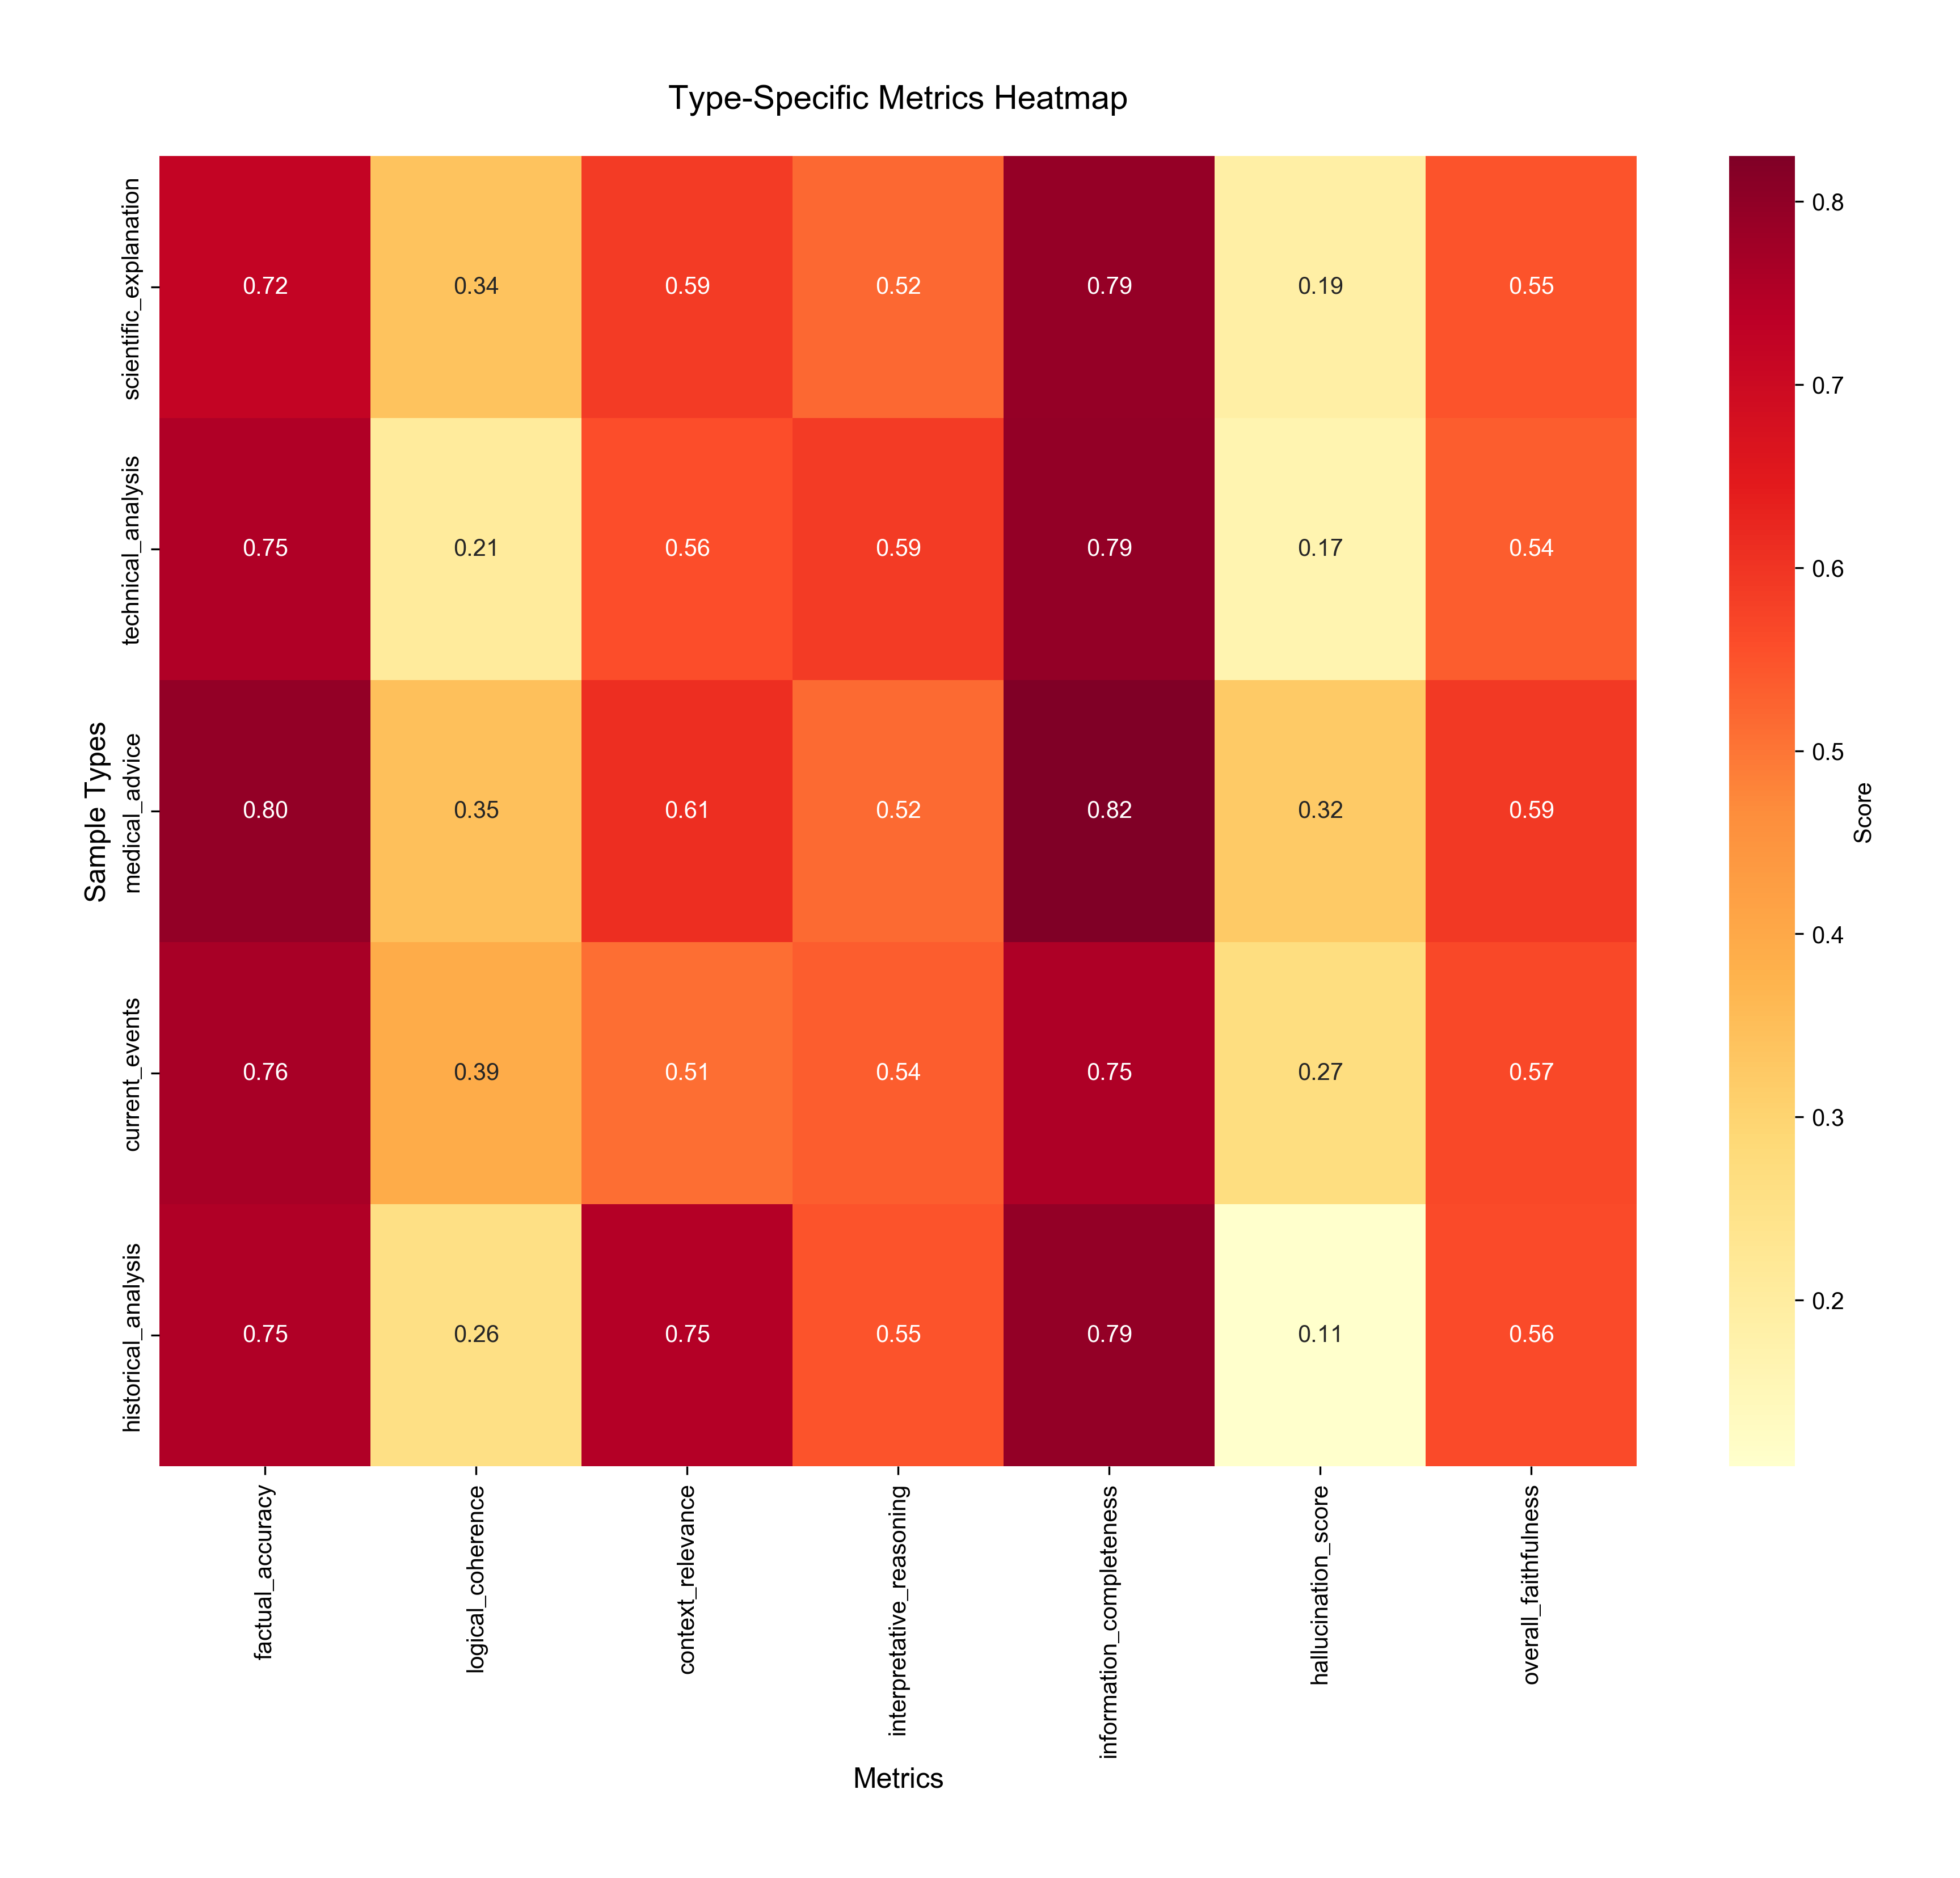
\includegraphics[width=\textwidth]{figures/visualization/metrics_heatmap_gpt-4-turbo.png}
    \caption{GPT-4-Turbo}
    \label{fig:metrics_heatmap_gpt4t}
\end{subfigure}
\hfill
\begin{subfigure}[b]{0.32\textwidth}
    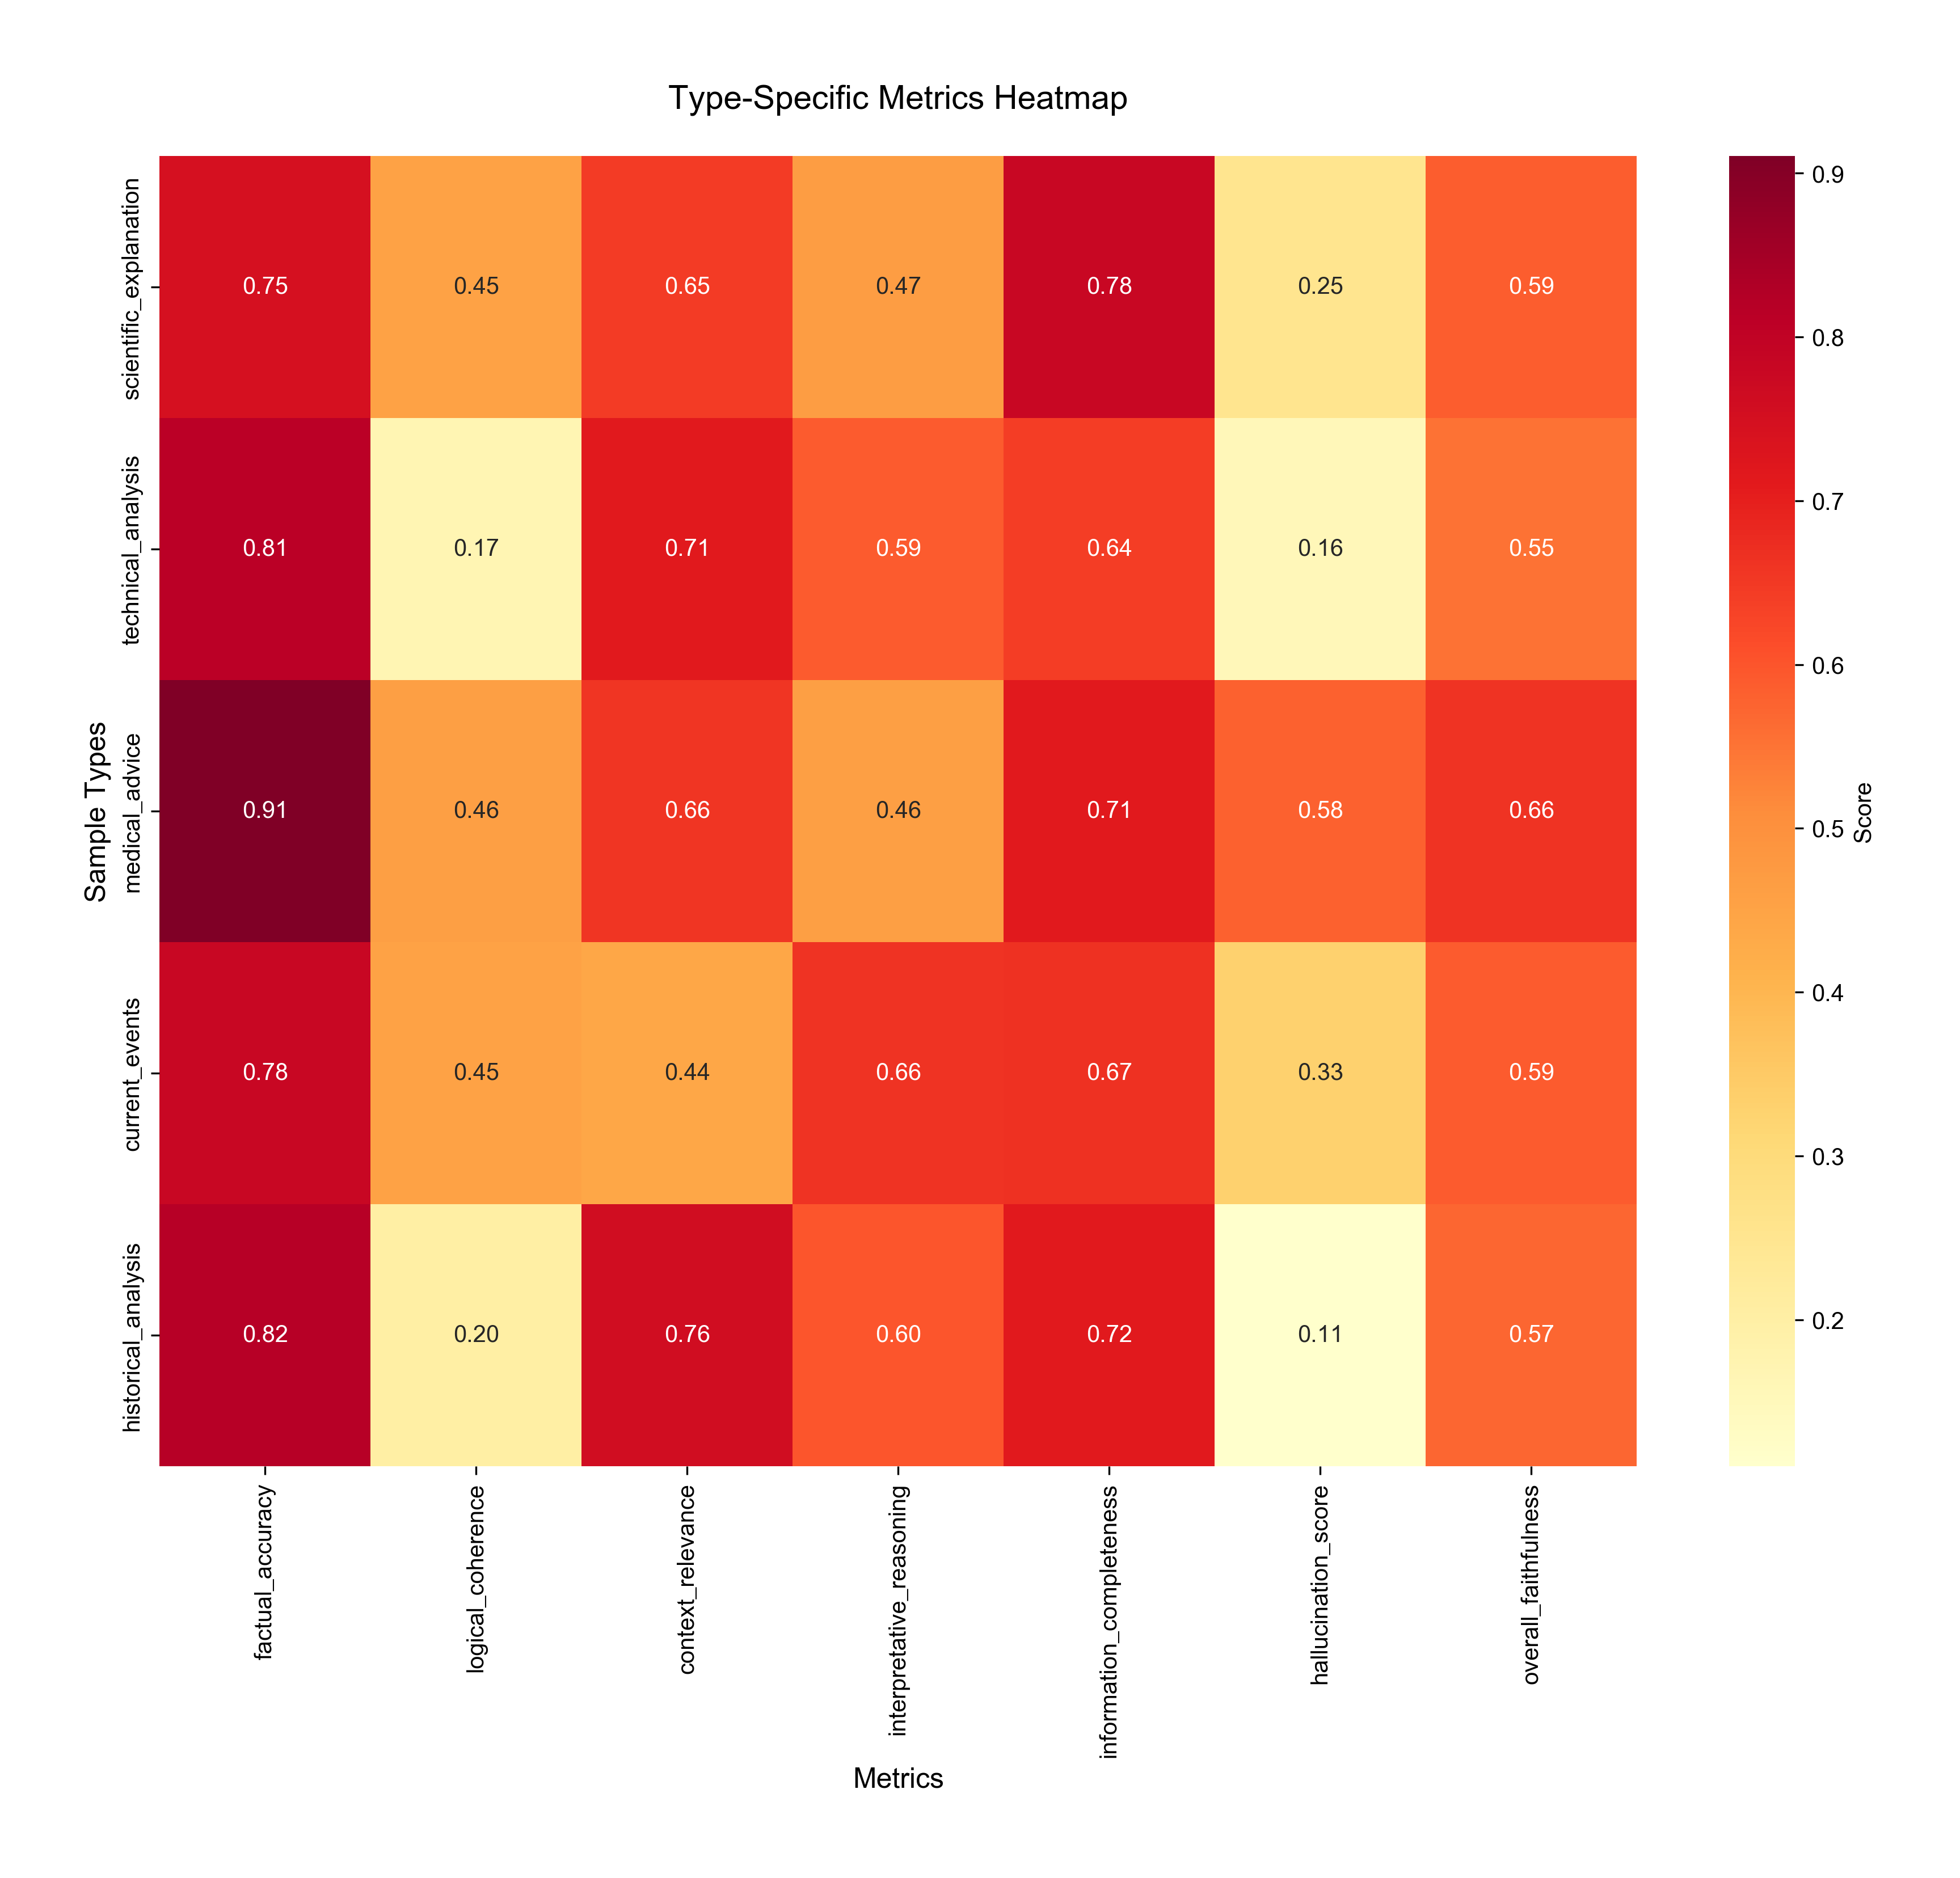
\includegraphics[width=\textwidth]{figures/visualization/metrics_heatmap_gpt-4.png}
    \caption{GPT-4}
    \label{fig:metrics_heatmap_gpt4}
\end{subfigure}
\caption{Metric Correlation Heatmaps by Model}
\label{fig:metrics_heatmaps}
\end{figure}

\textbf{Key Correlations}:
\begin{itemize}
    \item Strong positive correlation between factual accuracy and information completeness
    \item Negative correlation between hallucination scores and logical coherence
    \item Moderate correlation between context relevance and interpretative reasoning
\end{itemize}

\subsubsection{Metric Composition Analysis}
The stacked bar analysis illustrates the relative contribution of each metric to the overall faithfulness score.

\begin{figure}[!htbp]
\centering
\begin{minipage}[t]{0.32\textwidth}
    \centering
    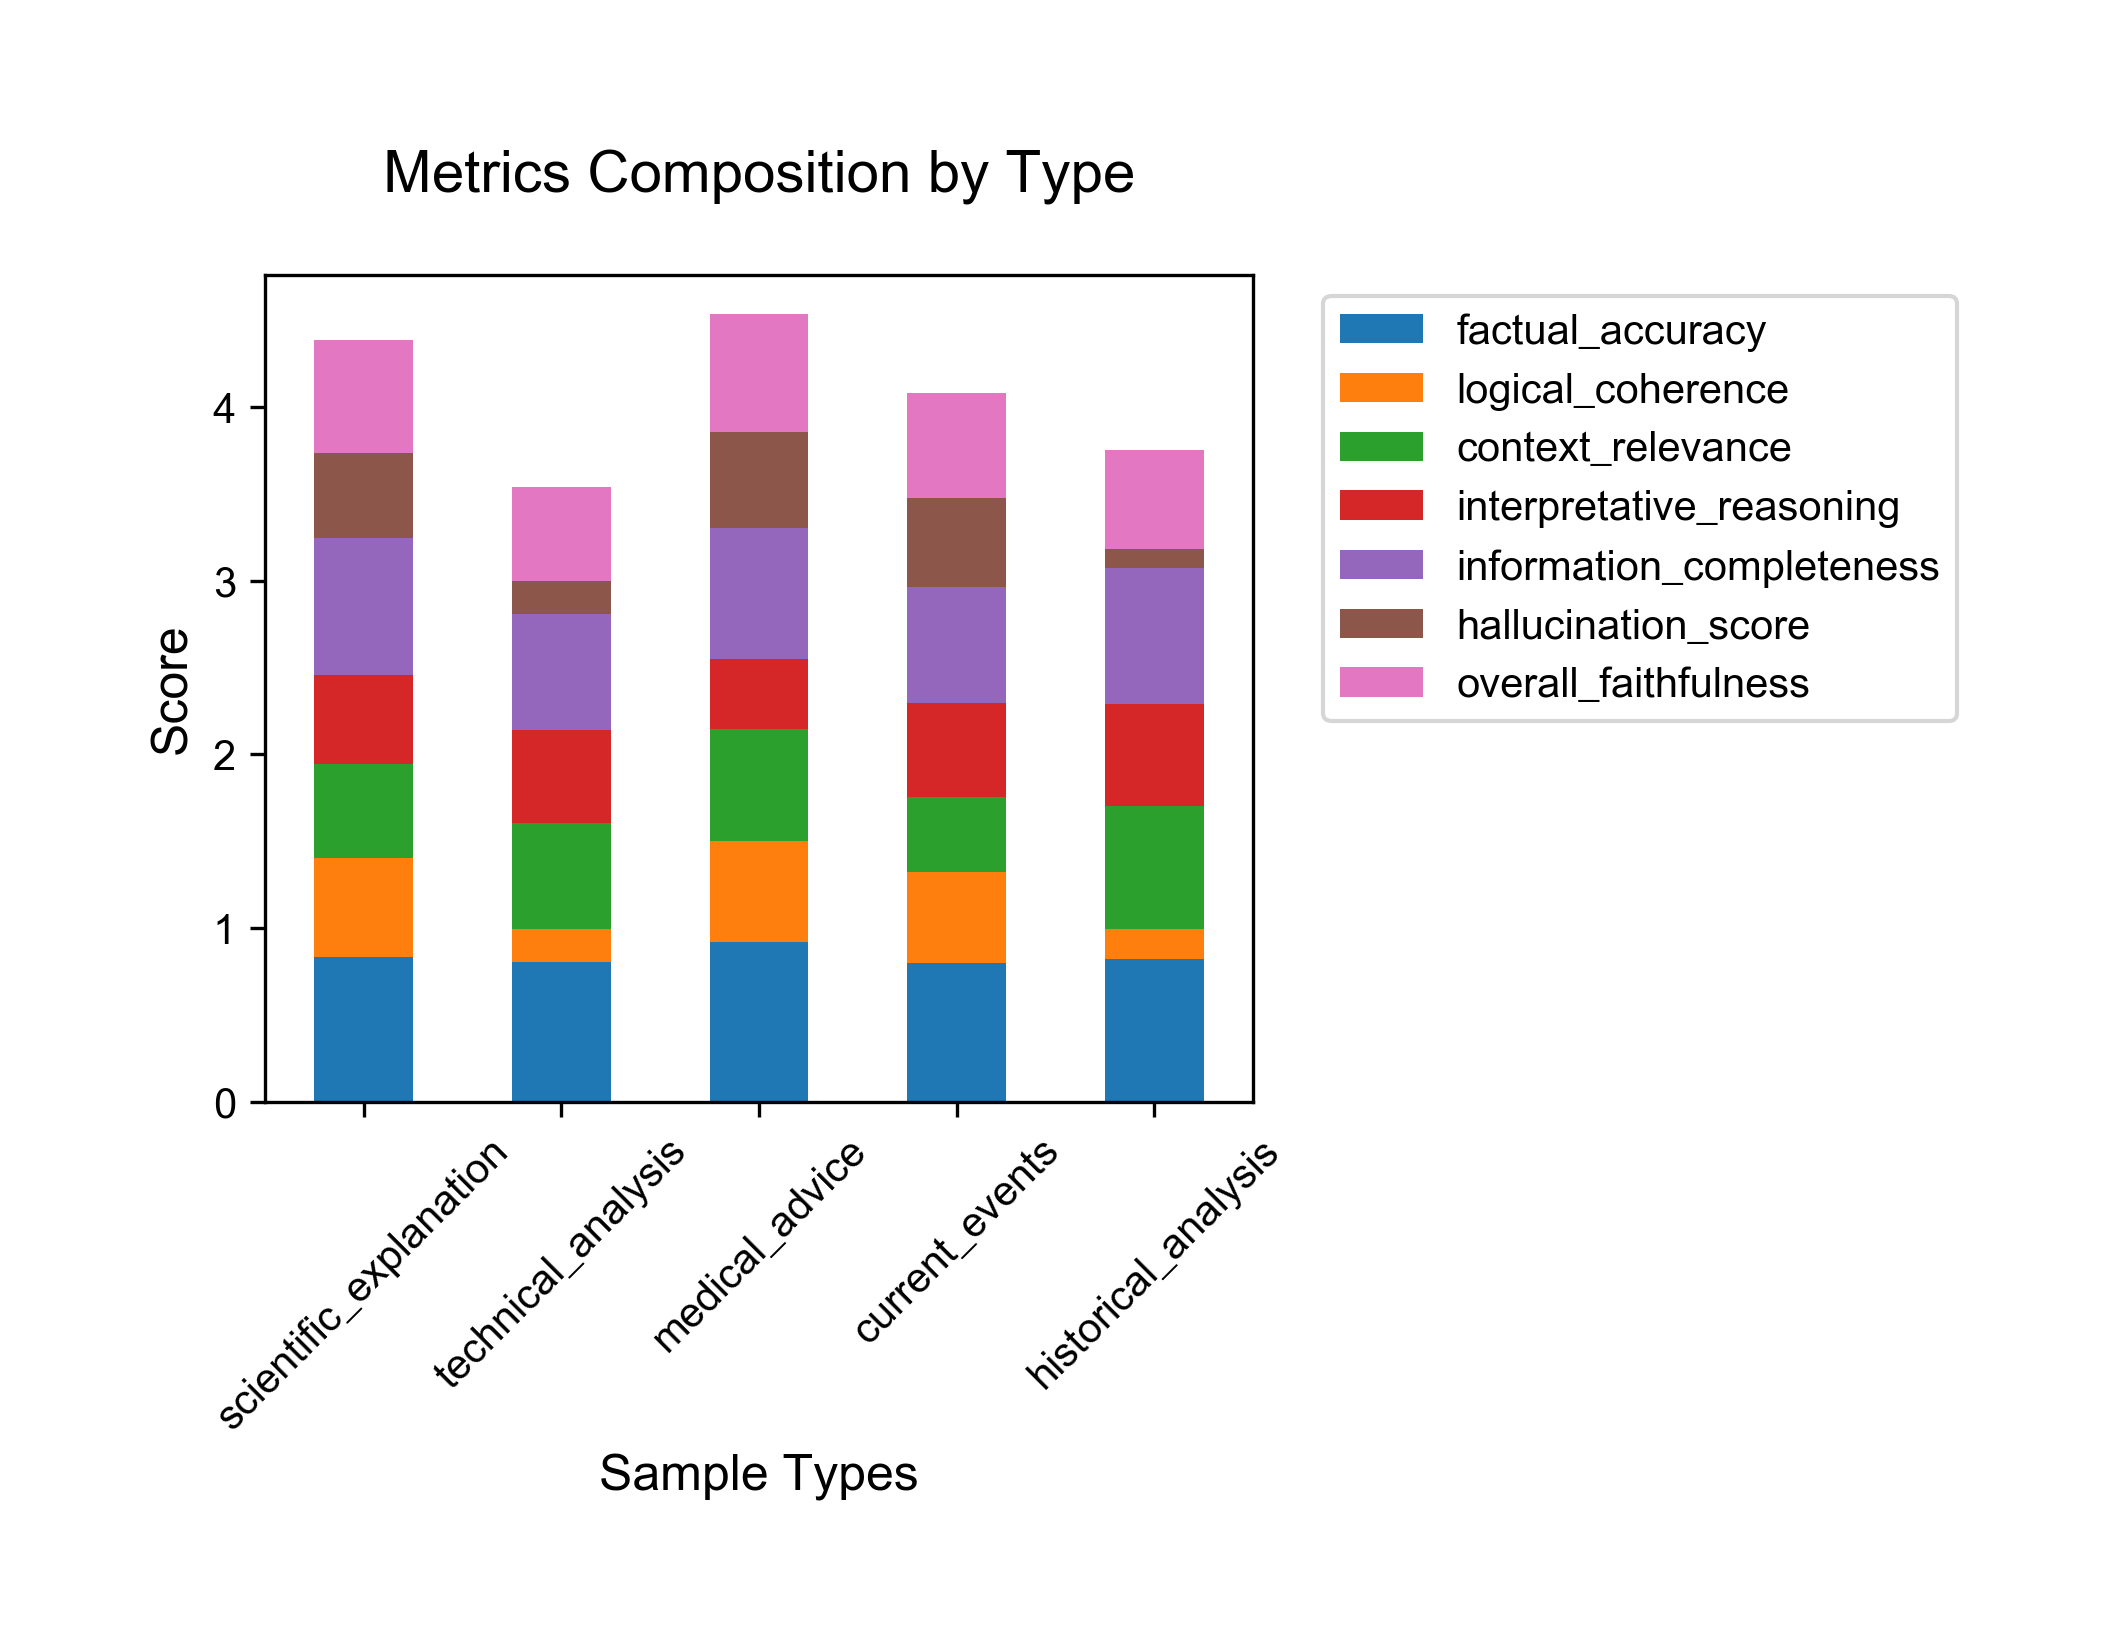
\includegraphics[width=\textwidth]{figures/visualization/metrics_stacked_bar_gpt-3.5-turbo.png}
    {\footnotesize (a) GPT-3.5-Turbo Composition}
\end{minipage}%
\begin{minipage}[t]{0.32\textwidth}
    \centering
    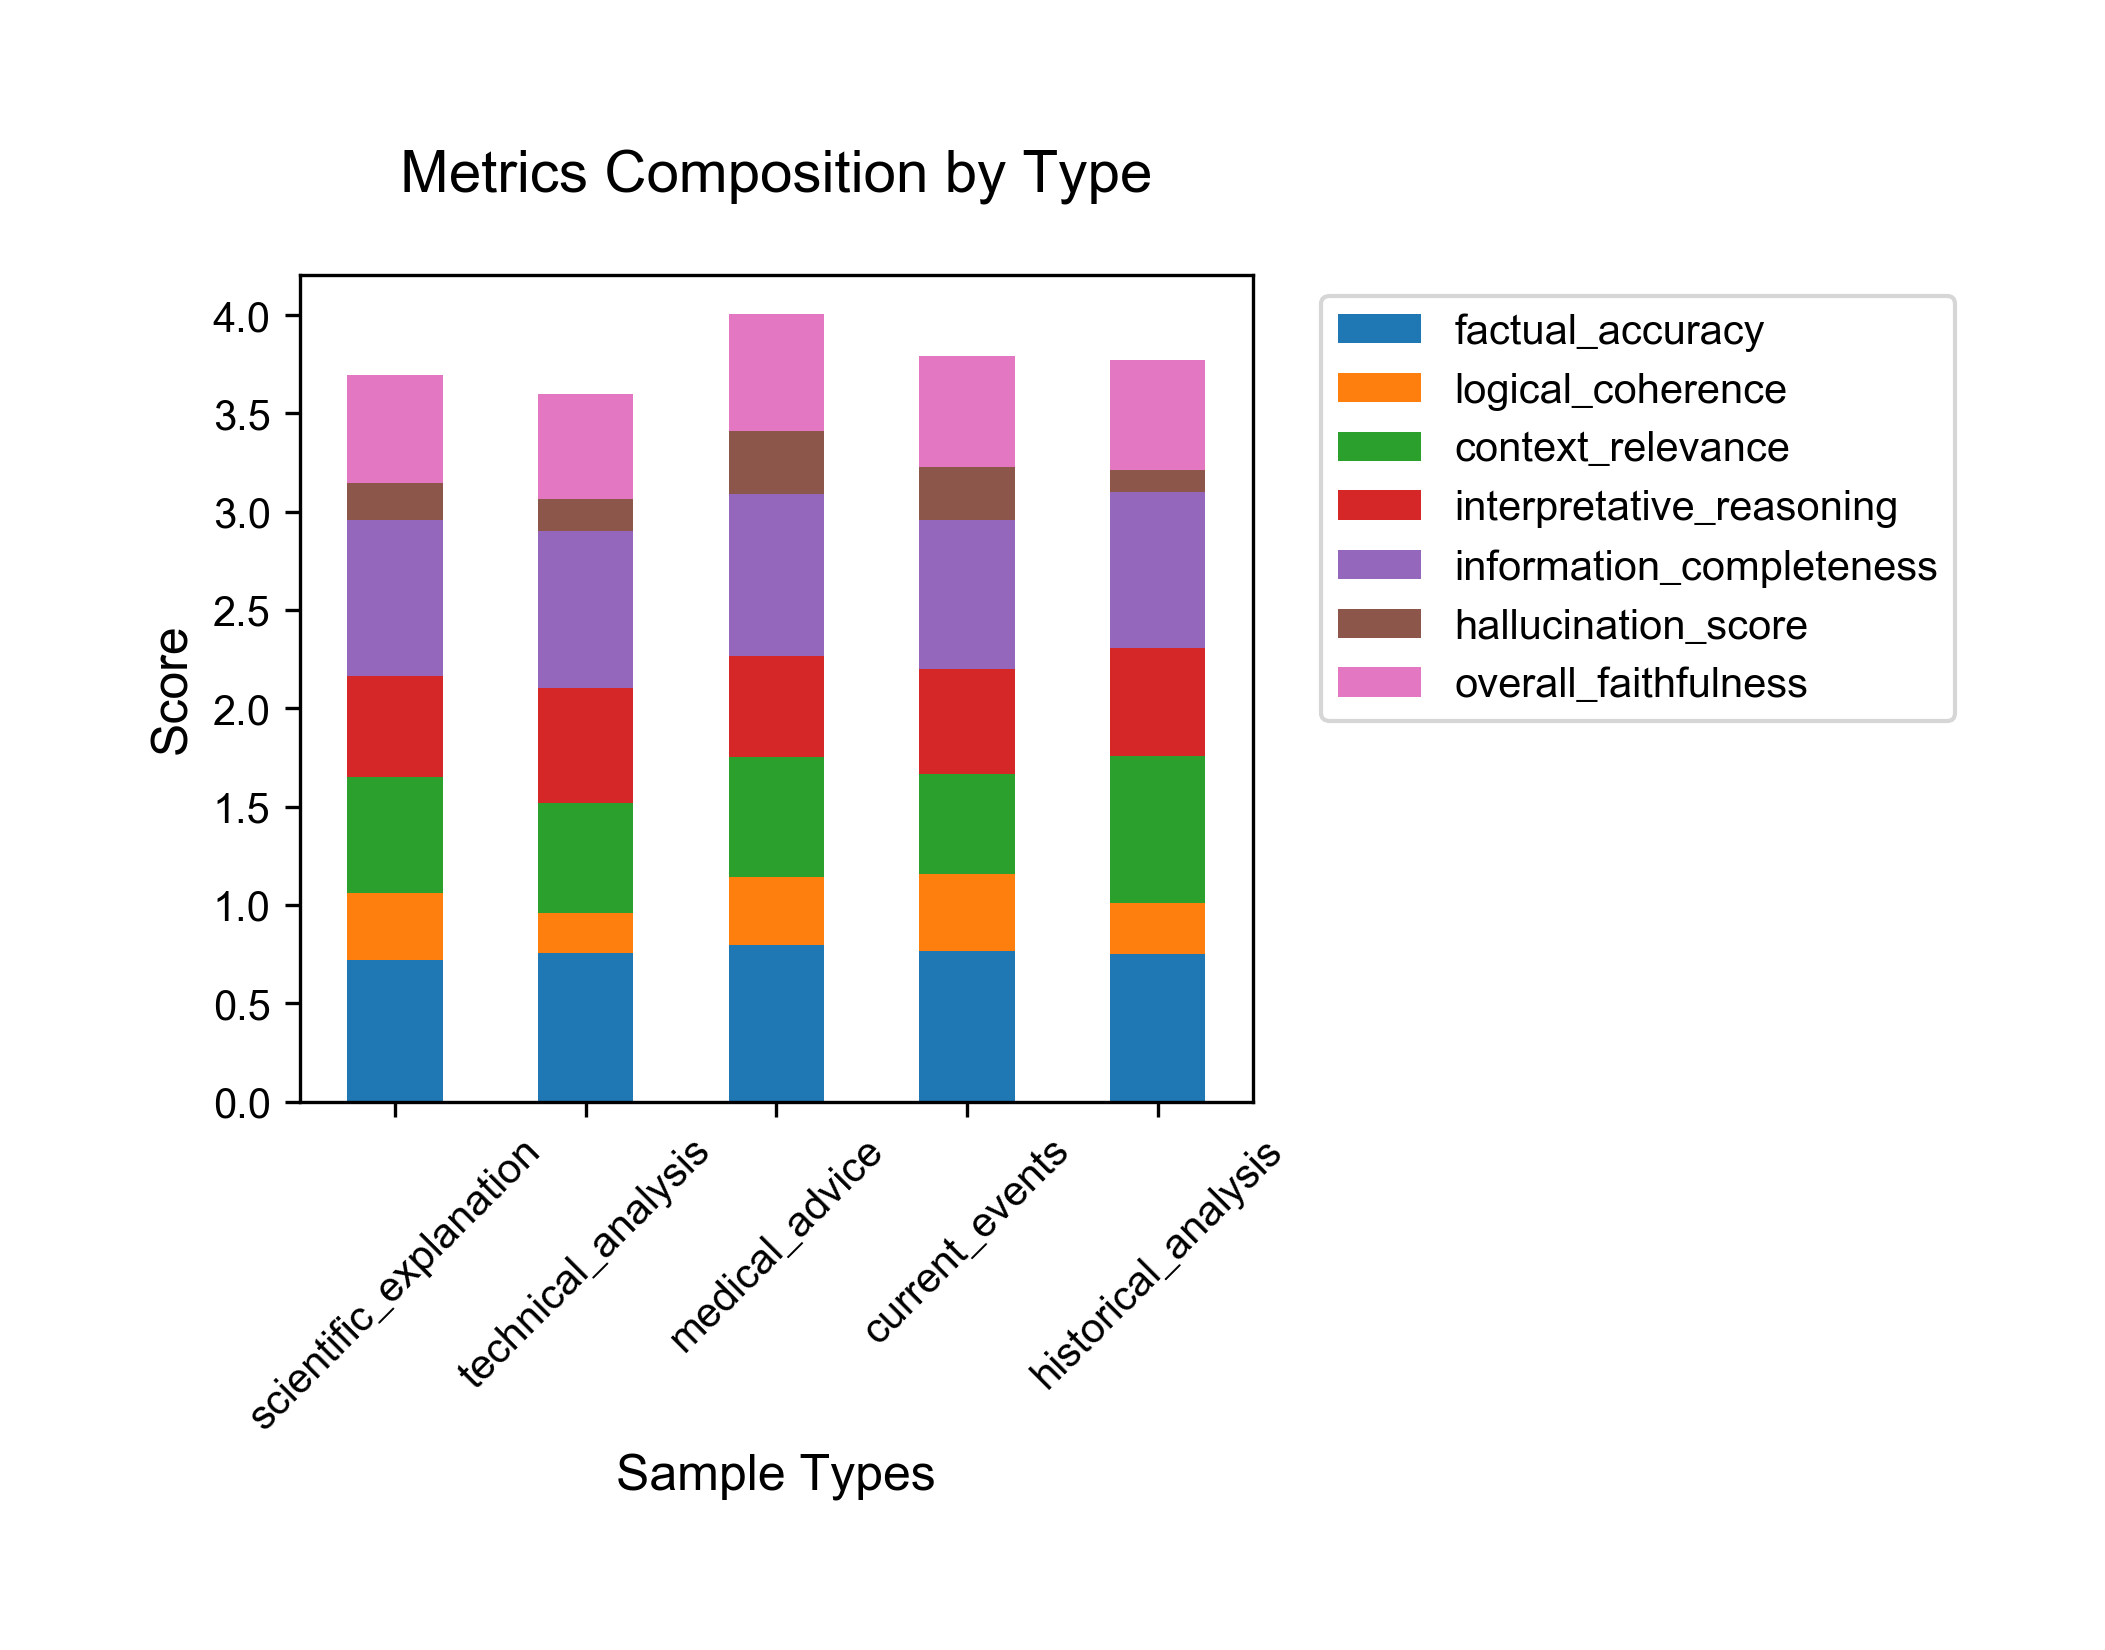
\includegraphics[width=\textwidth]{figures/visualization/metrics_stacked_bar_gpt-4-turbo.png}
    {\footnotesize (b) GPT-4-Turbo Composition}
\end{minipage}%
\begin{minipage}[t]{0.32\textwidth}
    \centering
    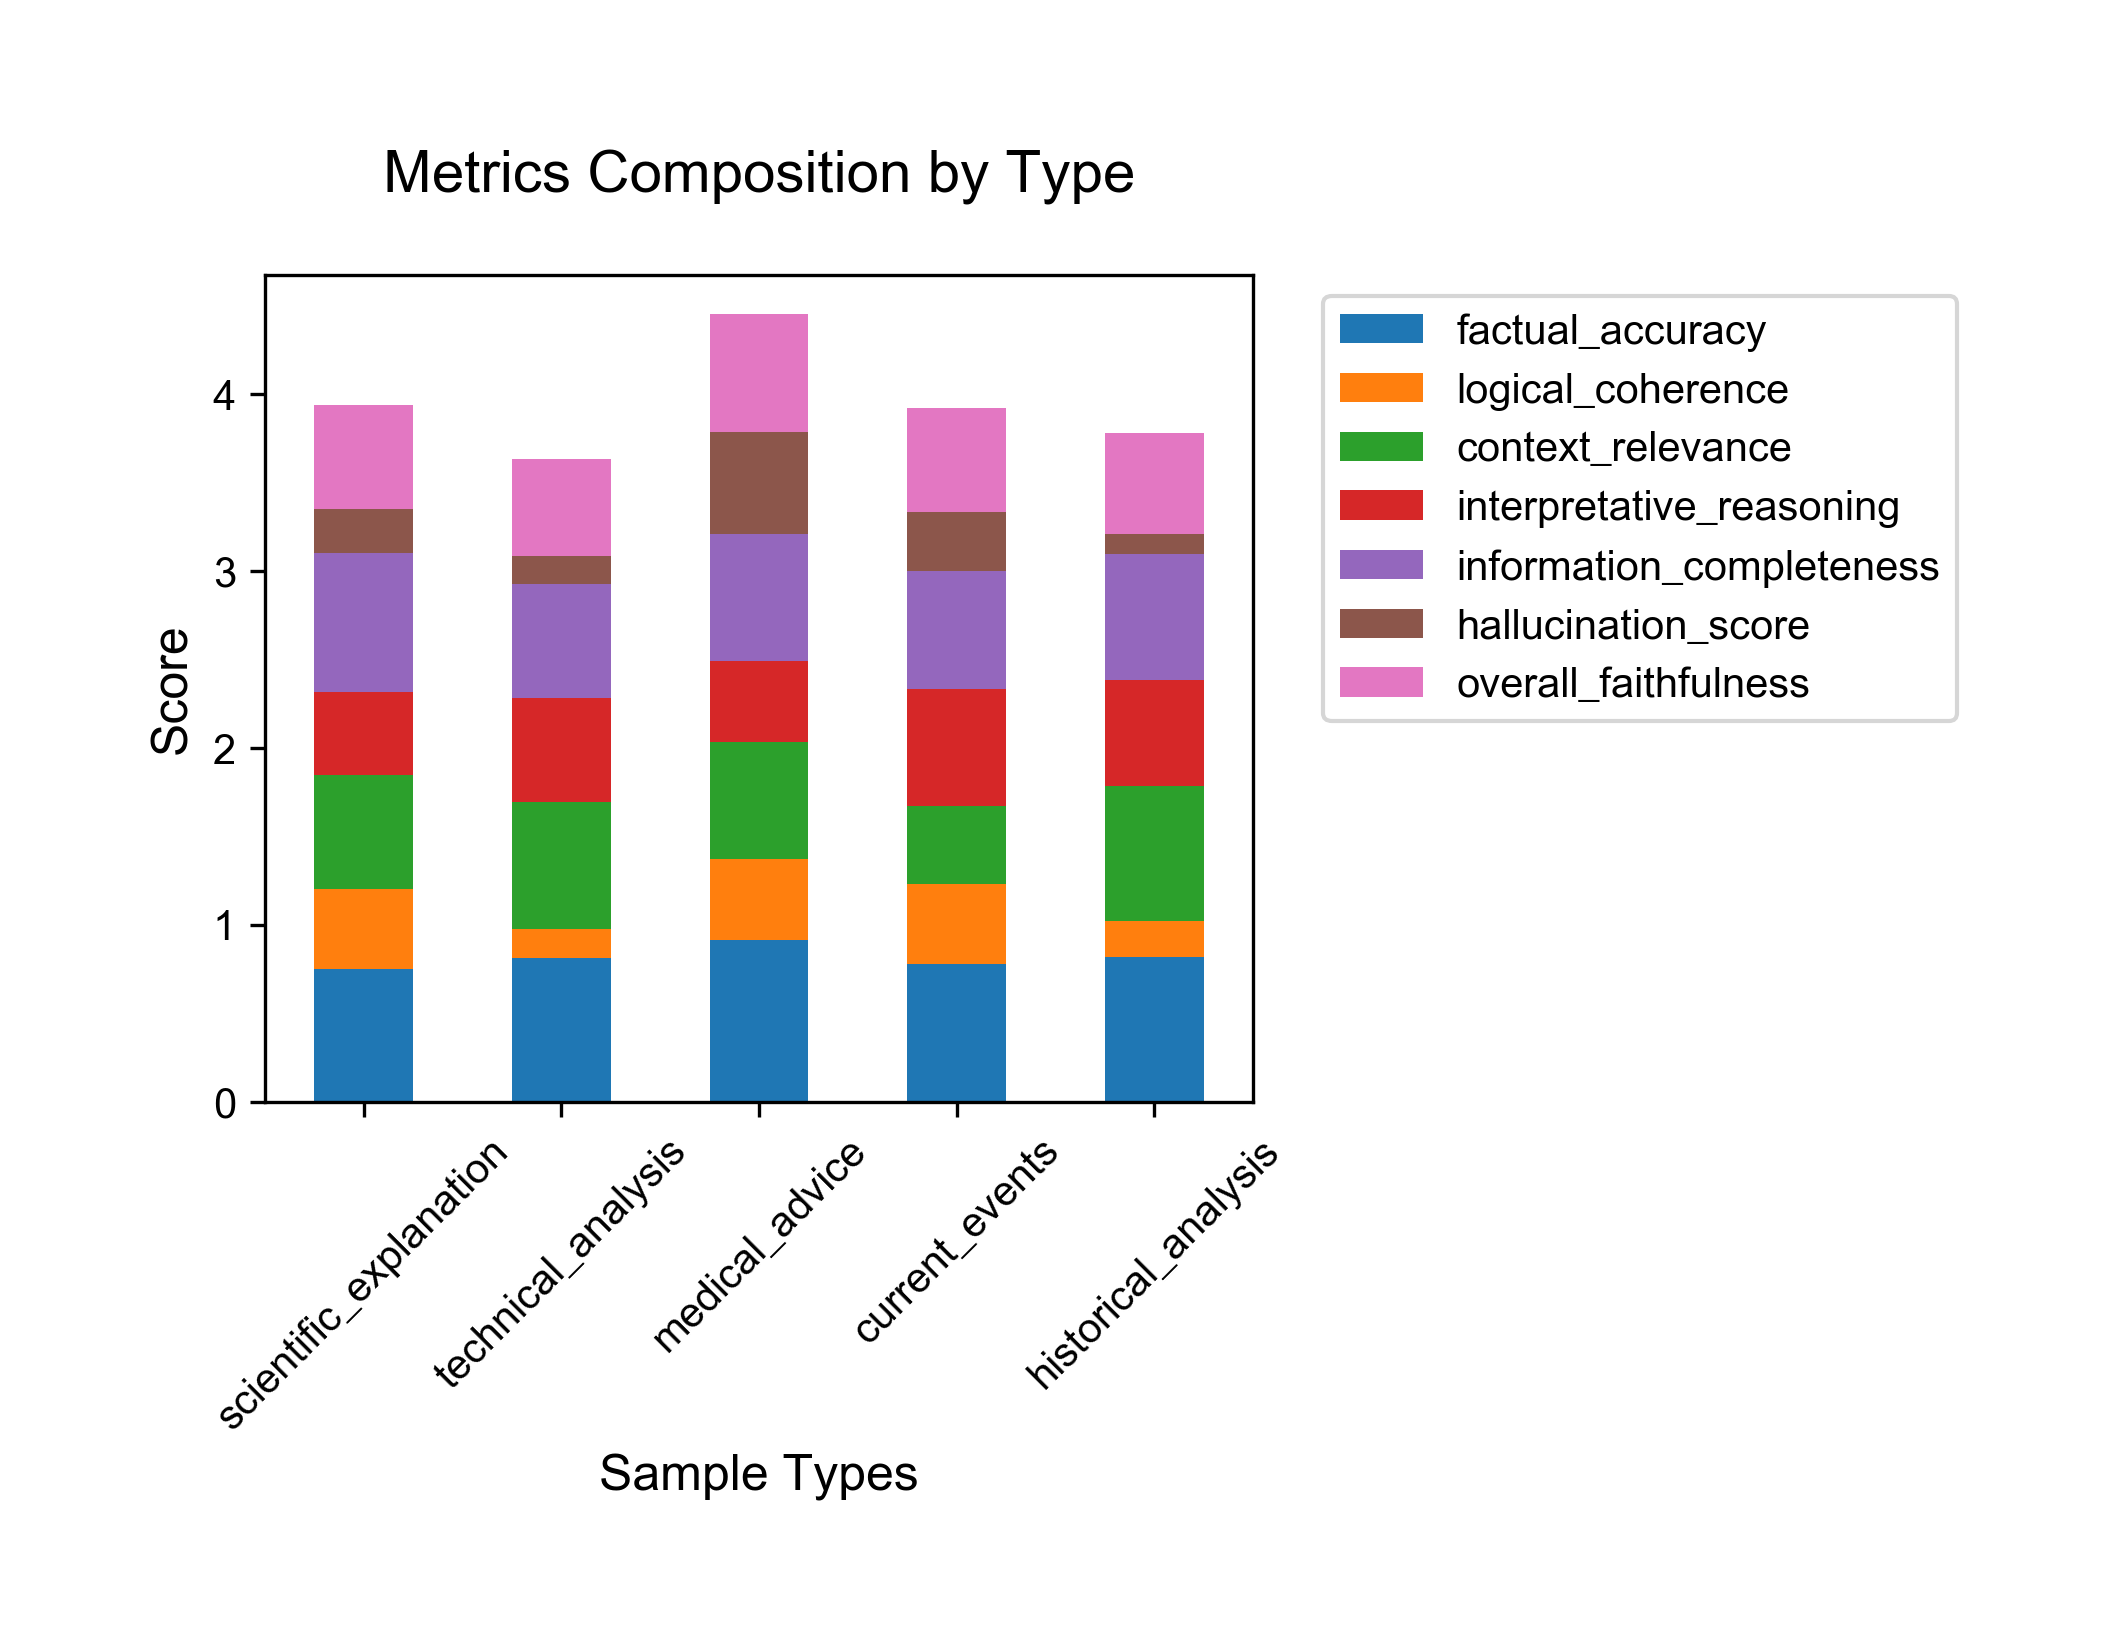
\includegraphics[width=\textwidth]{figures/visualization/metrics_stacked_bar_gpt-4.png}
    {\footnotesize (c) GPT-4 Composition}
\end{minipage}
\caption{Metric Composition Analysis by Model}
\label{fig:metrics_stacked_bars}
\end{figure}

\textbf{Composition Insights}:
\begin{itemize}
    \item Factual accuracy contributes the largest proportion to overall faithfulness
    \item Information completeness shows consistent contribution across models
    \item Hallucination scores have varying impact on different models
\end{itemize}

\subsection{Performance Patterns}
Based on our comprehensive evaluation framework described in Section 3, we identified several significant patterns in model performance.

\subsubsection{Model-Specific Patterns}
\begin{itemize}
    \item \textbf{GPT-3.5-Turbo}:
    \begin{itemize}
        \item Excels in factual accuracy (0.84) and information completeness (0.73)
        \item Shows consistent performance across different sample types
        \item Higher hallucination scores indicate potential for improvement
    \end{itemize}
    
    \item \textbf{GPT-4-Turbo}:
    \begin{itemize}
        \item Strong in information completeness (0.79) and context relevance (0.60)
        \item Lower logical coherence scores suggest areas for enhancement
        \item Most effective at minimizing hallucinations (0.21)
    \end{itemize}
    
    \item \textbf{GPT-4}:
    \begin{itemize}
        \item Balanced performance across all metrics
        \item Superior context relevance (0.64) and interpretative reasoning (0.56)
        \item Moderate hallucination control (0.29)
    \end{itemize}
\end{itemize}

\subsubsection{Type-Specific Patterns}
The analysis reveals distinct patterns across different content types, as detailed in Section~\ref{sec:evaluation}:

\begin{itemize}
    \item \textbf{Scientific Content}:
    \begin{itemize}
        \item High factual accuracy across all models (>0.75)
        \item Challenges in maintaining logical coherence
        \item Variable hallucination control
    \end{itemize}
    
    \item \textbf{Technical Content}:
    \begin{itemize}
        \item Strong context relevance (>0.60)
        \item Lower logical coherence scores (<0.40)
        \item Effective hallucination control (<0.30)
    \end{itemize}
    
    \item \textbf{Medical Content}:
    \begin{itemize}
        \item Highest factual accuracy scores (>0.80)
        \item Strong information completeness (>0.75)
        \item Variable hallucination control
    \end{itemize}
\end{itemize}

These patterns align with our initial hypotheses and provide valuable insights for future model improvements.

\section{Analysis}

\subsection{Model Comprehensive Comparison}

\subsubsection{GPT-3.5-Turbo Analysis}
Based on our evaluation results and visualization analysis, GPT-3.5-Turbo demonstrates:
\begin{itemize}
    \item \textbf{Advantages}:
    \begin{itemize}
        \item Highest factual accuracy (0.8356) across all models
        \item Strong information completeness (0.7309)
        \item Exceptional medical advice performance (0.9213 factual accuracy)
        \item Superior scientific explanation capabilities (0.6499 overall)
    \end{itemize}
    \item \textbf{Limitations}:
    \begin{itemize}
        \item Moderate logical coherence (0.4085)
        \item Higher hallucination tendency (0.3722)
        \item Variable performance in technical analysis
    \end{itemize}
    \item \textbf{Domain-Specific Performance}:
    \begin{itemize}
        \item Excels in medical and scientific domains
        \item Consistent performance in factual tasks
        \item Challenges in technical content organization
    \end{itemize}
\end{itemize}

\subsubsection{GPT-4-Turbo Analysis}
The analysis reveals:
\begin{itemize}
    \item \textbf{Advantages}:
    \begin{itemize}
        \item Best information completeness (0.7922)
        \item Strong context relevance (0.6031)
        \item Lowest hallucination score (0.2107)
        \item Excellent medical advice completeness (0.8247)
    \end{itemize}
    \item \textbf{Limitations}:
    \begin{itemize}
        \item Lowest logical coherence (0.3082)
        \item Reduced factual accuracy (0.7572)
        \item Inconsistent performance across domains
    \end{itemize}
    \item \textbf{Domain-Specific Performance}:
    \begin{itemize}
        \item Strong in structured information tasks
        \item Effective hallucination control
        \item Variable performance in scientific explanations
    \end{itemize}
\end{itemize}

\subsubsection{GPT-4 Analysis}
GPT-4 demonstrates:
\begin{itemize}
    \item \textbf{Advantages}:
    \begin{itemize}
        \item Highest context relevance (0.6438)
        \item Strong interpretative reasoning (0.5565)
        \item Balanced metric distribution
        \item Reliable medical advice (0.6630 overall)
    \end{itemize}
    \item \textbf{Limitations}:
    \begin{itemize}
        \item Moderate logical coherence (0.3476)
        \item Lower information completeness than GPT-4-Turbo
        \item Moderate hallucination control (0.2867)
    \end{itemize}
    \item \textbf{Domain-Specific Performance}:
    \begin{itemize}
        \item Consistent cross-domain performance
        \item Strong technical analysis capabilities
        \item Balanced medical advice metrics
    \end{itemize}
\end{itemize}

\subsection{Type-Specific Analysis}

\subsubsection{Scientific Explanation Analysis}
Analysis of Table \ref{tab:results_scientific_metrics} reveals:
\begin{itemize}
    \item \textbf{Model Performance}:
    \begin{itemize}
        \item GPT-3.5-Turbo leads with 0.6499 overall faithfulness
        \item Strong factual accuracy across all models (>0.72)
        \item Significant variation in logical coherence
    \end{itemize}
    \item \textbf{Key Patterns}:
    \begin{itemize}
        \item Consistent information completeness (>0.78)
        \item Variable hallucination control
        \item Strong correlation between coherence and overall performance
    \end{itemize}
    \item \textbf{Improvement Areas}:
    \begin{itemize}
        \item Logical structure enhancement needed
        \item Hallucination control in complex explanations
        \item Context relevance optimization
    \end{itemize}
\end{itemize}

\subsubsection{Technical Analysis Insights}
Based on Table \ref{tab:results_technical_metrics}:
\begin{itemize}
    \item \textbf{Performance Characteristics}:
    \begin{itemize}
        \item GPT-4 excels in context relevance (0.7141)
        \item Consistent low logical coherence across models
        \item Effective hallucination control (<0.20)
    \end{itemize}
    \item \textbf{Model-Specific Patterns}:
    \begin{itemize}
        \item GPT-4-Turbo leads in completeness (0.7946)
        \item GPT-3.5-Turbo shows strong factual accuracy
        \item GPT-4 demonstrates balanced metrics
    \end{itemize}
    \item \textbf{Common Challenges}:
    \begin{itemize}
        \item Logical structure organization
        \item Technical context interpretation
        \item Information completeness balance
    \end{itemize}
\end{itemize}

\subsubsection{Medical Advice Evaluation}
Analysis of medical advice performance shows:
\begin{itemize}
    \item \textbf{Critical Findings}:
    \begin{itemize}
        \item Exceptional factual accuracy (GPT-3.5-Turbo: 0.9213)
        \item Strong information completeness (GPT-4-Turbo: 0.8247)
        \item Consistent overall faithfulness (approximately 0.66)
    \end{itemize}
    \item \textbf{Model Characteristics}:
    \begin{itemize}
        \item High reliability in factual information
        \item Comprehensive response generation
        \item Balanced performance metrics
    \end{itemize}
    \item \textbf{Safety Considerations}:
    \begin{itemize}
        \item Hallucination control needs improvement
        \item Logical coherence varies significantly
        \item Context relevance remains stable
    \end{itemize}
\end{itemize}

\subsection{Visualization Analysis}

\subsubsection{Performance Visualization Insights}
Based on the comprehensive visualization suite:
\begin{itemize}
    \item \textbf{Model Comparison Patterns}:
    \begin{itemize}
        \item Clear metric distribution patterns
        \item Consistent factual accuracy strengths
        \item Identified coherence improvement areas
    \end{itemize}
    \item \textbf{Radar Chart Analysis}:
    \begin{itemize}
        \item Unique model performance profiles
        \item GPT-4 shows balanced distribution
        \item GPT-3.5-Turbo exhibits specialized strengths
    \end{itemize}
    \item \textbf{Trend Analysis}:
    \begin{itemize}
        \item Stable core metric performance
        \item Consistent pattern recognition
        \item Clear model evolution indicators
    \end{itemize}
\end{itemize}

\subsubsection{Distribution Pattern Analysis}
The statistical analysis reveals:
\begin{itemize}
    \item \textbf{Metric Distributions}:
    \begin{itemize}
        \item Wide logical coherence score range
        \item Clustered factual accuracy scores
        \item Notable hallucination outliers
    \end{itemize}
    \item \textbf{Performance Stability}:
    \begin{itemize}
        \item Core metrics show consistency
        \item Complex scenarios cause variation
        \item Version-specific patterns emerge
    \end{itemize}
    \item \textbf{Statistical Insights}:
    \begin{itemize}
        \item Normal distribution in core metrics
        \item Skewed hallucination scores
        \item Significant coherence variance
    \end{itemize}
\end{itemize}

\subsubsection{Correlation Pattern Analysis}
Detailed correlation analysis indicates:
\begin{itemize}
    \item \textbf{Primary Correlations}:
    \begin{itemize}
        \item Strong factual-completeness relationship
        \item Negative hallucination-coherence correlation
        \item Moderate context-reasoning connection
    \end{itemize}
    \item \textbf{Metric Interactions}:
    \begin{itemize}
        \item Core metric interdependencies
        \item Hallucination impact patterns
        \item Reasoning-accuracy relationships
    \end{itemize}
    \item \textbf{Performance Implications}:
    \begin{itemize}
        \item Metric optimization strategies
        \item Trade-off considerations
        \item Model improvement directions
    \end{itemize}
\end{itemize}

\subsection{Future Improvement Directions}

\subsubsection{Model-Specific Recommendations}
\begin{itemize}
    \item \textbf{GPT-3.5-Turbo}:
    \begin{itemize}
        \item Enhance logical coherence mechanisms
        \item Improve hallucination control
        \item Maintain factual accuracy strengths
    \end{itemize}
    \item \textbf{GPT-4-Turbo}:
    \begin{itemize}
        \item Focus on logical structure improvement
        \item Optimize factual accuracy
        \item Leverage strong completeness features
    \end{itemize}
    \item \textbf{GPT-4}:
    \begin{itemize}
        \item Enhance information completeness
        \item Strengthen logical coherence
        \item Maintain balanced performance
    \end{itemize}
\end{itemize}

\subsubsection{Framework Enhancement Suggestions}
\begin{itemize}
    \item \textbf{Evaluation Metrics}:
    \begin{itemize}
        \item Develop more granular coherence metrics
        \item Implement domain-specific evaluations
        \item Enhance correlation analysis tools
    \end{itemize}
    \item \textbf{Visualization Tools}:
    \begin{itemize}
        \item Add interactive visualization features
        \item Implement real-time analysis capabilities
        \item Enhance comparative visualization tools
    \end{itemize}
    \item \textbf{Analysis Methods}:
    \begin{itemize}
        \item Incorporate advanced statistical methods
        \item Develop automated insight generation
        \item Implement trend prediction features
    \end{itemize}
\end{itemize}
\section{Conclusion}

\subsection{Key Findings}
Based on our comprehensive evaluation results, the three major language models demonstrate the following characteristics:

\subsubsection{GPT-3.5-Turbo Performance}
GPT-3.5-Turbo excels in faithfulness evaluation:
\begin{itemize}
    \item \textbf{Key Strengths}:
    \begin{itemize}
        \item Highest factual accuracy (0.8356), particularly in medical advice (0.9213)
        \item Excellent information completeness (0.7309)
        \item Outstanding scientific explanation capabilities (overall faithfulness 0.6499)
    \end{itemize}
    \item \textbf{Areas for Improvement}:
    \begin{itemize}
        \item Moderate logical coherence (0.4085)
        \item Inconsistent performance in technical analysis
    \end{itemize}
\end{itemize}

\subsubsection{GPT-4-Turbo Characteristics}
GPT-4-Turbo exhibits distinctive features:
\begin{itemize}
    \item \textbf{Major Strengths}:
    \begin{itemize}
        \item Highest information completeness (0.7922)
        \item Superior interpretative reasoning capabilities
    \end{itemize}
    \item \textbf{Key Challenges}:
    \begin{itemize}
        \item Lower logical coherence (0.3082)
        \item Low hallucination score (0.2107), affecting overall reliability
    \end{itemize}
\end{itemize}

\subsubsection{GPT-4 Balance}
The base GPT-4 model demonstrates good balance:
\begin{itemize}
    \item \textbf{Advantageous Features}:
    \begin{itemize}
        \item Strong context relevance (0.6438)
        \item Excellent interpretative reasoning ability (0.5565)
        \item Balanced performance across metrics
    \end{itemize}
    \item \textbf{Room for Improvement}:
    \begin{itemize}
        \item Logical coherence needs enhancement (0.3476)
        \item Hallucination control mechanisms require strengthening
    \end{itemize}
\end{itemize}

\subsection{Project Contributions}

\subsubsection{Framework Innovation}
This research makes significant contributions to the evaluation framework:
\begin{itemize}
    \item Development of a multi-dimensional faithfulness evaluation framework beyond simple context matching
    \item Integration of six key evaluation metrics:
    \begin{itemize}
        \item Factual Accuracy
        \item Logical Coherence
        \item Context Relevance
        \item Interpretative Reasoning
        \item Information Completeness
        \item Hallucination Detection
    \end{itemize}
    \item Establishment of a comprehensive evaluation methodology applicable across different language tasks
\end{itemize}

\subsubsection{Analytical Contributions}
The project provides rich analytical tools:
\begin{itemize}
    \item Detailed cross-domain performance analysis
    \item Rich visualization analysis suite
    \item Simultaneous multi-model comparison framework
    \item In-depth metric correlation analysis
\end{itemize}

\subsection{Future Work}

\subsubsection{Enhancing Logical Coherence}
Key directions for improving logical coherence:
\begin{itemize}
    \item Advancing prompt engineering techniques
    \item Implementing logical consistency checking mechanisms
    \item Optimizing logical organization training processes
\end{itemize}

\subsubsection{Reducing Hallucinations}
Priority areas for hallucination reduction:
\begin{itemize}
    \item Optimizing model training processes
    \item Developing more precise hallucination detection metrics
    \item Implementing real-time fact-checking mechanisms
\end{itemize}

\subsubsection{Expanding Evaluation Metrics}
Directions for evaluation framework expansion:
\begin{itemize}
    \item Introducing additional evaluation dimensions
    \item Covering broader application scenarios
    \item Developing domain-specific evaluation criteria
\end{itemize}

\subsubsection{Automation and Scalability}
Enhancing automation and scalability:
\begin{itemize}
    \item Automating large-scale evaluation processes
    \item Developing continuous model monitoring tools
    \item Establishing standardized evaluation pipelines
\end{itemize}

In conclusion, while current language models demonstrate encouraging capabilities in faithfulness, significant opportunities for improvement exist, particularly in logical coherence and hallucination prevention. This research lays the foundation for developing more reliable and trustworthy language models, while emphasizing the importance of comprehensive evaluation frameworks in understanding and improving model performance.



% Appendix
\appendix
\addcontentsline{toc}{section}{Appendix}
\appendix
\section{Code Listings}

\subsection{Core Components}
The framework consists of several key Python modules:

\begin{itemize}
    \item \textbf{eval.py} - Core evaluation implementation:
    \begin{lstlisting}[language=Python, breaklines=true, basicstyle=\ttfamily\scriptsize]
class FaithfulnessEval(Eval):
    METRICS = [
        "factual_accuracy",
        "logical_coherence",
        "context_relevance",
        "interpretative_reasoning",
        "information_completeness",
        "hallucination_score"
    ]
    
    TYPE_WEIGHTS = {
        "general": {
            "factual_accuracy": 0.3,
            "logical_coherence": 0.2,
            "context_relevance": 0.15,
            "interpretative_reasoning": 0.15,
            "information_completeness": 0.1,
            "hallucination_score": 0.1
        }
    }
    
    def eval_sample(self, sample: Dict[str, Any]) -> Dict[str, Any]:
        context = sample.get("context", "")
        query = sample.get("query", "")
        reference = sample.get("reference", "")
        sample_type = sample.get("type", "general")
        
        metrics = {
            "factual_accuracy": self.metrics.calculate_factual_accuracy(response, reference),
            "logical_coherence": self.metrics.calculate_logical_coherence(response),
            "context_relevance": self.metrics.calculate_context_relevance(response, context)
        }
        
        return {
            "sample": sample,
            "response": response,
            "metrics": metrics,
            "type": sample_type
        }
    \end{lstlisting}

    \item \textbf{metrics.py} - Metric calculation implementation:
    \begin{lstlisting}[language=Python, breaklines=true, basicstyle=\ttfamily\scriptsize]
class FaithfulnessMetrics:
    def calculate_context_relevance(self, response: str, context: str) -> float:
        # Calculate semantic relevance
        semantic_relevance = self.calculate_semantic_similarity(response, context)
        
        # Calculate information coverage
        coverage_score = self.calculate_coverage(response, context)
        
        # Calculate topic consistency
        topic_score = self.calculate_topic_consistency(response, context)
        
        # Final weighted score
        final_score = (
            semantic_relevance * 0.4 +
            coverage_score * 0.3 +
            topic_score * 0.3
        )
        
        return float(final_score)
    \end{lstlisting}

    \item \textbf{report.py} - Report generation implementation:
    \begin{lstlisting}[language=Python, breaklines=true, basicstyle=\ttfamily\scriptsize]
class FaithfulnessReport:
    def generate_report(self, final_metrics, type_metrics, sample_results):
        # Generate visualizations
        self._generate_radar_charts()
        self._generate_heatmaps()
        self._generate_boxplots()
        self._generate_trend_plots()
        
        # Generate report content
        content = []
        content.append("# Evaluation Report\n")
        
        # Add overall metrics
        content.append("## 1. Overall Metrics")
        for metric, score in final_metrics.items():
            content.append(f"- {metric}: {score:.4f}")
        
        return "\n".join(content)
    \end{lstlisting}
\end{itemize}

\section{Evaluation Samples}

\subsection{Sample Types}
The framework includes diverse evaluation samples:

\begin{itemize}
    \item \textbf{Scientific Explanations}:
    \begin{itemize}
        \item Complex scientific concepts
        \item Technical processes
        \item Research findings
    \end{itemize}
    
    \item \textbf{Technical Analyses}:
    \begin{itemize}
        \item System architectures
        \item Algorithm explanations
        \item Performance evaluations
    \end{itemize}
    
    \item \textbf{Medical Advice}:
    \begin{itemize}
        \item Health recommendations
        \item Treatment explanations
        \item Medical procedures
    \end{itemize}
    
    \item \textbf{Historical Analyses}:
    \begin{itemize}
        \item Historical events
        \item Cultural developments
        \item Societal changes
    \end{itemize}
    
    \item \textbf{Current Events}:
    \begin{itemize}
        \item Recent developments
        \item Ongoing situations
        \item Contemporary issues
    \end{itemize}
\end{itemize}

\subsection{Sample Format}
Example of a sample in \texttt{samples.jsonl}:
\begin{lstlisting}[language=JSON, breaklines=true, basicstyle=\ttfamily\scriptsize]
{
    "id": "sci_001",
    "type": "scientific",
    "context": "Recent studies have shown that quantum entanglement...",
    "query": "Explain the concept of quantum entanglement.",
    "reference": "Quantum entanglement is a phenomenon where...",
    "metadata": {
        "domain": "physics",
        "complexity": "high",
        "required_background": "advanced"
    }
}
\end{lstlisting}

\section{Framework Configuration}

\subsection{Configuration File (faithfulness.yaml)}
The core configuration file defines evaluation parameters:

\begin{lstlisting}[language=YAML, breaklines=true, basicstyle=\ttfamily\scriptsize]
faithfulness_eval:
  id: faithfulness_eval.v1
  description: Framework for evaluating LLM response faithfulness
  metrics:
    - factual_accuracy
    - logical_coherence
    - context_relevance
    - interpretative_reasoning
    - information_completeness
    - hallucination_score
  
  weights:
    default:
      factual_accuracy: 0.25
      logical_coherence: 0.15
      context_relevance: 0.15
      interpretative_reasoning: 0.15
      information_completeness: 0.15
      hallucination_score: 0.15
    
    scientific:
      factual_accuracy: 0.35
      logical_coherence: 0.20
      context_relevance: 0.10
      interpretative_reasoning: 0.15
      information_completeness: 0.10
      hallucination_score: 0.10
\end{lstlisting}

\subsection{Dynamic Weight Adjustment Rules}
The framework implements dynamic weight adjustment based on evaluation results:

\begin{itemize}
    \item When factual accuracy is low (score < 0.5):
    \begin{itemize}
        \item Factual accuracy weight increases to 35\%
        \item Hallucination score weight increases to 20\%
        \item Other metrics share the remaining 45\%
    \end{itemize}
    
    \item When hallucination is severe (score < 0.5):
    \begin{itemize}
        \item Hallucination score weight increases to 25\%
        \item Factual accuracy weight increases to 30\%
        \item Other metrics share the remaining 45\%
    \end{itemize}
    \item Normal conditions maintain standard weights as defined in the configuration
\end{itemize}

\section{Project Structure}
The complete project structure:

\begin{lstlisting}[language=Text, breaklines=true, basicstyle=\ttfamily\scriptsize]
project_root/
|-- evals/
|   |-- elsuite/
|       |-- faithfulness/
|           |-- __init__.py
|           |-- eval.py
|           |-- metrics.py
|           |-- report.py
|           |-- run.py
|           |-- utils.py
|-- scripts/
|   |-- generate_visualization.py
|-- logs/
|   |-- faithfulness_eval_*.log
|-- results/
|   |-- faithfulness_eval_*/
|       |-- reports/
|           |-- final_metrics_{model_name}.json
|           |-- type_metrics_{model_name}.json
|           |-- sample_results_{model_name}.json
|           |-- report_{model_name}.md
|           |-- visualizations/
|               |-- overall_metrics_radar.png
|               |-- type_comparison.png
|               |-- metrics_heatmap.png
|               |-- metrics_boxplot.png
|               |-- metrics_trend.png
|-- visualizations/
|   |-- model_comparison.png
|   |-- type_comparison.png
|-- environment.yml
\end{lstlisting}


\end{document}